% ---- ETD Document Class and Useful Packages ---- %
\documentclass{ucetd}
\usepackage{booktabs}
\usepackage{amsfonts}
\usepackage{amsthm}
\usepackage{epsfig, minted}
%\usepackage[utf8x]{inputenc}
\usepackage{amsmath}
\let\Bbbk\relax
\usepackage{amssymb}
\usepackage{algorithm}
\usepackage{algorithmicx}
\usepackage[noend]{algpseudocode}
\usepackage{enumitem}      % adjust spacing in enums
%\usepackage{subfig}
\usepackage{caption}
\usepackage{subcaption}
\usepackage{multirow}
\usepackage{rotating}
\usepackage{wrapfig}
\usepackage{tabu}
\usepackage{cleveref}
\usepackage{array}
\usepackage{pifont}
\usepackage[normalem]{ulem}

%% Use these commands to set biographic information for the title page:
\title{Capitalizing on Security, Performance, and Energy Tradeoffs in Full Drive Encryption Schemes for Fun and Profit}
\author{Bernard Dickens III}
\department{Computer Science}
\division{Physical Sciences}
\degree{Doctor of Philosophy}
\date{August 2020}

%% Use these commands to set a dedication and epigraph text
\dedication{To my kiddos (whom at the time of writing do not yet exist): I find
the courage to peer over the edge of human knowledge and reach down into that
abyss of the unknown with the hope that you may one day benefit from my
struggles. I can't wait to meet you!}
%\epigraph{Epigraph Text}

%% Custom additions

%enumitem settings
\setlist{
  listparindent=\parindent,
  parsep=0pt,
}

% Fancy subsection references with cref
\crefformat{section}{\S#2#1#3} % see manual of cleveref, section 8.2.1
\crefformat{subsection}{\S#2#1#3}
\crefformat{subsubsection}{\S#2#1#3}

% Flexible table column specifications
\newcolumntype{C}[1]{>{\centering\arraybackslash}m{#1}}

\usepackage[natbib=true,backend=bibtex,firstinits=true,style=numeric-comp,sorting=nyt,defernumbers,maxnames=99,maxcitenames=99]{biblatex}
\usepackage{balance}
\usepackage{adjustbox}

\addbibresource{refs.bib}

\usepackage{pgfplots}

\pgfplotsset{compat=1.8,compat/show suggested version=false}
\usetikzlibrary{plotmarks}
\usetikzlibrary{calc}

\pgfplotsset{
   /pgfplots/bar  cycle  list/.style={/pgfplots/cycle  list={%
        {black,fill=black!30!white,mark=none},%
        {black,fill=red!30!white,mark=none},%
        {black,fill=green!30!white,mark=none},%
        {black,fill=yellow!30!white,mark=none},%
        {black,fill=brown!30!white,mark=none},%
     }
   },
}

\usetikzlibrary{external}
\tikzexternalize[prefix=out/]
\tikzexternalize

\usetikzlibrary{patterns}
\usepgfplotslibrary{groupplots}
\pgfplotsset{
   every axis label/.append style={font=\small},
   tick label style={font=\small},
}

\pgfkeys{
    /pgf/number format/precision=1,
    /pgf/number format/fixed zerofill=true,
}

%% Custom colors that are colorblind safe, print friendly, and photocopy safe
\definecolor{purpleDark}{RGB}{94, 60, 153}
\definecolor{purpleLight}{RGB}{178, 171, 210}
\definecolor{orangeDark}{RGB}{230, 97, 1}
\definecolor{orangeLight}{RGB}{253, 184, 99}

%% Other custom colors
\definecolor{gray}{gray}{0.75}

% Ability to filter the values plotted from tables via `discard if not` key
\pgfplotsset{
    discard if symbol/.style 2 args={
        x filter/.append code={
            \edef\tempa{\thisrow{#1}}
            \edef\tempb{#2}
            \ifx\tempa\tempb
                \def\pgfmathresult{inf}
            \fi
        }
    }
}

\pgfplotsset{
    discard if symbol not/.style 2 args={
        x filter/.append code={
            \edef\tempa{\thisrow{#1}}
            \edef\tempb{#2}
            \ifx\tempa\tempb
            \else
                \def\pgfmathresult{inf}
            \fi
        }
    }
}

\pgfplotsset{
    discard if number/.style 2 args={
        x filter/.append code={
            \ifdim\thisrow{#1} pt=#2pt
                \def\pgfmathresult{inf}
            \fi
        }
    }
}

\pgfplotsset{
    discard if number not/.style 2 args={
        x filter/.append code={
            \ifdim\thisrow{#1} pt=#2pt
            \else
                \def\pgfmathresult{inf}
            \fi
        }
    }
}

\pgfplotsset{
    nodes near coords greater equal only/.style={
        small value/.style={
            /tikz/coordinate,
        },
        every node near coord/.append style={
            check for small values/.code={
                \begingroup
                \pgfkeys{/pgf/fpu}
                \pgfmathparse{\pgfplotspointmeta<#1}
                \global\let\result=\pgfmathresult
                \endgroup
                \pgfmathfloatcreate{1}{1.0}{0}
                \let\ONE=\pgfmathresult
                \ifx\result\ONE
                    \pgfkeysalso{/pgfplots/small value}
                \fi
            },
            check for small values
        },
    },
}

\pgfplotsset{
    nodes near coords greater only/.style={
        small value/.style={
            /tikz/coordinate,
        },
        every node near coord/.append style={
            check for small values/.code={
                \begingroup
                \pgfkeys{/pgf/fpu}
                \pgfmathparse{\pgfplotspointmeta<=#1}
                \global\let\result=\pgfmathresult
                \endgroup
                \pgfmathfloatcreate{1}{1.0}{0}
                \let\ONE=\pgfmathresult
                \ifx\result\ONE
                    \pgfkeysalso{/pgfplots/small value}
                \fi
            },
            check for small values
        },
    },
}

\algnewcommand{\LineComment}[1]{\(\triangleright\) #1}

% some useful shortcuts
\newcommand{\ie}{\textit{i.e., }}
\newcommand{\eg}{\textit{e.g., }}
\newcommand{\CC}{C\nolinebreak\hspace{-.05em}\raisebox{.5ex}{\tiny\bf +}\nolinebreak\hspace{-.10em}\raisebox{.5ex}{\tiny\bf +}}

% units for results
\newcommand{\us}{\,$\mu$s}
\newcommand{\ms}{\,ms}
\newcommand{\KB}{\,KB}
\newcommand{\MB}{\,MB}
\newcommand{\GB}{\,GB}
\newcommand{\MHz}{\,MHz}
\newcommand{\GHz}{\,GHz}

% new latex commands:
%   Remove long section
\newcommand{\PUNT}[1]{}
\newcommand{\TABLETWO}[1]{}
%   Label work to be done
\definecolor{gray}{gray}{0.75}
\newcommand{\TODO}[1]{\textcolor{gray}{\textbf{\ [TODO:\ #1]\ }}}
\newcommand{\TR}[1]{#1}
\newcommand{\FIX}[1] {\textcolor{red}{\textbf{\ [FIX:\ #1]\ }}}
%   Referencing various pieces of the document:
\newcommand{\figref}[1]{Fig.~\ref{fig:#1}}
\newcommand{\figsref}[2]{Figures~\ref{fig:#1} and~\ref{fig:#2}}
\newcommand{\figrref}[2]{Figures~\ref{fig:#1}--\ref{fig:#2}}
\newcommand{\secref}[1]{Section~\ref{sec:#1}}
\newcommand{\secsref}[2]{Sections~\ref{sec:#1} and~\ref{sec:#2}}
\newcommand{\eqnref}[1]{Eqn.~\ref{eqn:#1}}
\newcommand{\eqnsref}[2]{Equations~\ref{eqn:#1} and~\ref{eqn:#2}}
\newcommand{\eqnrref}[2]{Equations~\ref{eqn:#1}--\ref{eqn:#2}}
\newcommand{\insref}[1]{Instruction~\ref{ins:#1}}
\newcommand{\tblref}[1]{Table~\ref{tbl:#1}}
\newcommand{\appref}[1]{Appendix~\ref{app:#1}}

\newcommand{\algoref}[1]{Algorithm~\ref{algo:#1}}

\makeatletter
\newcommand\footnoteref[1]{\protected@xdef\@thefnmark{\ref{#1}}\@footnotemark}
\makeatother

% Custom hyphenation rules

%\DeclareMathOperator{\minimize}{minimize}
%\DeclareMathOperator{\st}{s.t.}
%\DeclareMathOperator*{\argmin}{arg\,min}
%\DeclareMathOperator*{\argmax}{arg\,max}
\newcommand{\argmin}{\arg\!\min}
\newcommand{\argmax}{\arg\!\max}
\newcommand{\minimize}{minimize}
\newcommand{\optimize}{optimize}
\newcommand{\ceil}[1]{\lceil #1 \rceil}
\newcommand{\floor}[1]{\lfloor #1 \rfloor}
\newcommand{\st}{s.t.}

\newcommand{\StrongBoxURI}{https://github.com/Xunnamius/strongbox-switchcrypt}
\newcommand{\SwitchCryptURI}{https://github.com/Xunnamius/strongbox-switchcrypt}

% \pdfstringdefDisableCommands{
%     \def\\{}
%     \def\unskip{}
%     \def\texttt#1{<#1>}
% }

%-------------------------------------------------------------------------

\begin{document}
%% Basic setup commands
% If you don't want a title page comment out the next line and uncomment the line after it:
\maketitle
%\omittitle

% These lines can be commented out to disable the copyright/dedication/epigraph pages
\makecopyright
\makededication
% \makeepigraph

%% Make the various tables of contents
\tableofcontents
\listoffigures
\listoftables

\acknowledgments
This material is based upon work supported by the National Science Foundation
under Grant No. CNS-1526304. I would first and foremost like to thank my primary
advisor, Dr. Henry (Hank) Hoffmann. Without his compassion, patience, and wealth
of experience, none of this work would have been possible. I'd like to thank my
committee members Dr. Ariel J. Feldman (Applied Crypto), Dr. Haryadi S. Gunawi
(Filesystems), and Dr. David Cash (Crypto Theory) for all their hard work.
Hopefully I spelled everyone's names correctly this time!

I'd also like to acknowledge my former students Richard Anthony Alvarez and
Trevor James Medina for their contributions to HASCHK. Of course, I'd like to
acknowledge my mother Michelle Davis who throughout my childhood \emph{always}
had money for Computer Science workbooks (but not McDonalds!), my father for
always having my best interests at heart, my inspiring siblings, Zara for the
infinity life lessons, Jeff Holmes of the old Chicago Broadway Armory for
showing an eight-year-old me just how fun and powerful computers can be, Von
Steuben high school Computer Science teachers Stirling Crow and Andres Hernandez
for teaching me web design and gifting me the wisdom to ``use my powers for
good,'' my coach Audra Anderson and the BDPA for teaching me humility and how to
be an effective and engaging teacher, Dr. Rahmelle Thompson of the Morehouse
College Hopps Scholars program for revealing my trajectory to me, Dr. Adrienne
Raglin of the Department of Defense Army Research Laboratory for putting up with
me (twice!) and teaching me what real research looks like, the University of
Chicago and all its faculty and staff for fostering a culture of socially
conscious elite intellectual pursuit, President Barack H. Obama and Senator
Elizabeth Warren for demonstrating black excellence and how to persist
nevertheless, and all my PhD colleagues, mentors, former students, and true
friends over the years for their unwavering support throughout this process.

Know I would not have made it without you all.

\abstract
The security of data at rest---widely understood as FDE or Full-Drive
Encryption---is an important concern among several in modern computer systems.
These concerns exist in contention over a set of finite resources. For instance:
a device that is battery-constrained must remain within its energy budget which
may change over time, e.g. when a device enters ``battery-saver mode'';
regardless, this device must meet certain performance guarantees or the user
experience will suffer; above all, the data on the device must be secure from
adversaries; and the device has a finite amount of drive space available. At any
given moment we trade battery life for performance, performance for security,
security for drive space, and so on. Unfortunately, designing a FDE system that
can navigate such treacherous tradeoffs efficiently, effectively, and with
respect to performance and security guarantees is entirely non-trivial. This
dissertation explores this space of tradeoffs and how we might optimize for one
concern without violating another given kernel and/or user space in-context
invariants that might shift over time.

Full-drive encryption is especially important for mobile devices because they
contain large quantities of sensitive data yet are easily lost or stolen. As
this research demonstrates, the standard approach to FDE—the AES block cipher in
XTS mode—is 3-5x slower than unencrypted storage. Authenticated encryption based
on stream ciphers is already used as a faster alternative to AES in other
contexts, such as HTTPS, but the conventional wisdom is that stream ciphers are
unsuitable for FDE. Used naively in drive encryption, stream ciphers are
vulnerable to attacks, and mitigating these attacks with on-drive metadata is
generally believed to ruin performance.

We address the difficulty of using stream ciphers for FDE with StrongBox, a
stream cipher based FDE layer that is a drop-in replacement for dm-crypt, the
standard Linux FDE module based on AES-XTS. StrongBox introduces a system design
and on-drive data structures that exploit certain properties of filesystems to
avoid costly rekeying penalties and a counter stored in trusted hardware to
protect against attacks. We implement StrongBox and SwitchCrypt on an ARM
big.LITTLE mobile processor and test its performance under multiple popular
production filesystems.

We push the envelope further with SwitchCrypt, a software mechanism that allows
us to move beyond merely making stream ciphers available for FDE. SwitchCrypt
enables practical navigation of the tradeoff space made by balancing competing
security and latency requirements via \emph{cipher switching} in space or time.
Our key insight in achieving low-overhead switching is to leverage the
overwrite-averse, append-mostly behavior of underlying solid-state storage to
trade throughput for reduced energy use and/or certain security properties.
Similar to StrongBox, we implement SwitchCrypt on an ARM big.LITTLE mobile
processor and test its performance under the popular F2FS LFS. We provide
empirical results demonstrating the conditions under which different switching
strategies are optimal through the exploration of four cases studies.

Finally, with HASCHK, we consider the same stream cipher based cryptographic
primitives in an alternative domain: data \emph{in motion} rather than at rest.
Specifically: securing data downloads over the internet. Such downloads come
with many risks, including the chance that the resource has been corrupted, or
that an attacker has replaced your desired resource with a compromised version.
The de facto standard for addressing this risk is the use of \emph{checksums}
coupled with a secure transport layer; users download a resource, compute its
checksum, and compare that with an authoritative checksum. Problems with this
approach include (1) \emph{user apathy}---for most users, calculating and
verifying the checksum is too tedious; and (2) \emph{co-hosting}---an attacker
who compromises a resource can trivially compromise a checksum hosted on the
same system. The co-hosting problem remains despite advancements in tools that
automate checksum verification and generation. In this dissertation we propose
\emph{HASCHK}, a resource verification protocol expanding on de facto
checksum-based integrity protections to defeat co-hosting while automating the
tedious parts of checksum verification to secure ``data in motion'' downloads
over the internet.

StrongBox, SwitchCrypt, and HASCHK together demonstrate that security is indeed
a paramount concern and valid dimension with which to trade off alongside other
tier-one concerns without compromising data security or requiring obscene
performance sacrifices, all while staying within a shifting energy budget.


\mainmatter
% Main body of text follows

\chapter{Introduction} \label{chp:introduction}

\section{Thesis Statement}

With this research into filesystem, device driver, and hardware Flash
Translation Layer (FTL) based Full Disk Encryption (FDE) schemes for ``data at
rest'', we primarily consider: (1) the established wisdom in the crypto
community that stream ciphers are unsuitable for FDE and (2) exploring the
tradeoff space made between total energy use, filesystem performance, and
reasonable security guarantees when comparing specific cipher configurations. In
the first case, we develop and implement a secure approach to FDE based on
stream ciphers, the proliferation of secure hardware, and the characteristics of
Log-Structured Filesystems (LFS). In the second case, we implement a dozen
stream ciphers---each exposing several knobs---and demonstrate navigating our
tradeoff space via runtime cipher switching while maintaining reasonable
security guarantees. We then present a formal analysis of our system's security
guarantees. Finally, we consider data authenticity schemes using some of the
same cryptographic primitives but in the context of ``data in motion'' through
the development and implementation of a resource verification protocol expanding
on de facto checksum-based integrity protections to defeat co-hosting while
automating the tedious parts of checksum verification.

\section{Contributions}

\subsection{StrongBox}

StrongBox is a novel scheme for securing data at rest and is a drop-in
replacement for AES-XTS-backed FDE such as dm-crypt~\cite{dmcrypt}. StrongBox
uses a fast stream cipher for confidentiality and performance with integrity
preserving Message Authentication Codes~\cite{MAC} and a secure, persistent
hardware counter to ensure integrity and counter the weaknesses inherent in
stream cipher based FDE. With StrongBox's, we present a system design enabling
the first confidential, high-performance drive encryption scheme based on stream
ciphers.

\subsection{SwitchCrypt}

SwitchCrypt is software mechanism that navigates the tradeoff space made by
balancing competing security and latency requirements via \emph{cipher
switching} in space or time and represents a vastly improved FDE approach based
on StrongBox. SwitchCrypt addresses the reality that optimizing for performance
often conflicts with other key concerns like energy usage and desired security
properties. SwitchCrypt leverages the behavior of underlying solid-state storage
to trade between throughput, energy use, and desirable security properties of
various ciphers. This is accomplished dynamically and at run time.

\subsection{HASCHK}

HASCHK is a resource verification protocol expanding on de facto checksum-based
integrity protections to defeat co-hosting while automating the tedious parts of
checksum verification. HASCHK mitigates the authenticity risks of data in
motion; in this instance: downloading resources over the internet. We find our
approach is more effective than existing mitigation methods, significantly
raises the bar for the attacker, and is deployable at scale.

\section{Related Work} \label{sec:sc-related}

The standard approach to FDE, using AES-XTS, introduces significant overhead.
Recently, it has been established that encryption using \emph{stream ciphers}
for FDE is faster than using AES~\cite{StrongBox}, but in practice it is
non-trivial. Prior work explores several approaches: a non-deterministic CTR
mode (Freestyle~\cite{Freestyle}), a length-preserving ``tweakable
super\\-pseudorandom permutation'' (Adiantum~\cite{Adiantum}), and a stream cipher
in a binary additive (XOR) mode leveraging LFS overwrite-averse behavior to
prevent overwrites (StrongBox~\cite{StrongBox}).

Unlike StrongBox and other work, which focuses on optimizing performance despite
re-ciphering due to overwrites, SwitchCrypt maintains overwrite protections
while abstracting the idea of re-encrypting nuggets out into cipher switching;
instead of myopically pursuing a performance win, we can pursue energy/battery
and security wins as well.

Further, trading off security for energy, performance, and other concerns is not
a new research area~\cite{ScalableSecurity, WolterReinecke, ZengChow1,
HaleemEtAl, LiOmiecinski, Merkel4, Merkle3}. Goodman et al. introduced
selectively decreasing the security of some data to save
energy~\cite{ScalableSecurity}. However, their approach is designed for
communication and only considered iteration/round count, thus it did not
anticipate the need for SwitchCrypt's generic interface, switching strategies,
or security scores. Wolter and Reinecke study approaches to quantifying security
in several contexts~\cite{WolterReinecke}. This study anticipates the value of
dynamically switching ciphers but proposes no mechanisms to enable this in FDE.
Similarly, companies like LastPass and Google have explored performance-security
tradeoffs. Google's Adiantum (above) uses a less secure reduced round version of
ChaCha~\cite{Adiantum}. While not an FDE solution, LastPass has dealt with
scaling the number of iterations of PBKDF\#2, trading performance for security
during login sessions~\cite{LastPass}.


\chapter{StrongBox: Using Stream Ciphers for High Performance Full Drive Encryption} \label{chp:strongbox}
\section{Motivation} \label{sec:sb-motivation}

Full drive encryption (FDE)\footnote{The common term is full \emph{disk}
encryption, but this work targets SSDs, so we use \emph{drive}.} is an essential
technique for protecting the privacy of data at rest. For mobile devices,
maintaining data privacy is especially important as these devices contain
sensitive personal and financial data yet are easily lost or stolen. The current
standard for securing data at rest is to use the AES cipher in XTS
mode~\cite{XTS, NISTXTS}. Unfortunately, employing AES-XTS increases read/write
latency by 3--5$\times$ compared to unencrypted storage.

It is well known that authenticated encryption using \emph{stream}
ciphers---such as ChaCha20~\cite{ChaCha20}---is faster than using AES (see
\figref{motivation}). Indeed, Google made the case for stream ciphers over AES,
switching HTTPS connections on Chrome for Android to use a stream cipher for
better performance~\cite{google-blog}. Stream ciphers are not used for FDE,
however, for two reasons: (1) confidentiality and (2) performance. First, when
applied naively to stored data, stream ciphers are trivially vulnerable to
attacks---including \emph{many-time pad and rollback attacks}---that reveal the
plaintext by overwriting a secure storage location with the same key. Second, it
has been assumed that adding the meta-data required to resist these attacks
would ruin the stream cipher's performance advantage. Thus, the conventional
wisdom is that FDE necessarily incurs the overhead of AES-XTS or a similar
primitive.

We argue that two technological shifts in mobile device hardware overturn this
conventional wisdom, enabling confidential, high-performance storage with stream
ciphers. First, these devices commonly employ solid-state storage with Flash
Translation Layers (FTL), which operate similarly to Log-structured File Systems
(LFS)~\cite{LFS,F2FS,NILFS}. Second, mobile devices now support trusted
hardware, such as Trusted Execution Environments (TEE)~\cite{TEE,TrustZone} and
secure storage areas~\cite{eMMC-standard}. FTLs and LFSes are used to limit
sector/cell overwrites, hence extending the life of the drive. Most writes
simply appended to a log, reducing the occurrence of overwrites and the chance
for attacks. The presence of secure hardware means that drive encryption modules
have access to persistent, monotonically increasing counters that can be used to
prevent rollback attacks when overwrites do occur.

Given these trends, we propose StrongBox, a new method for securing data at
rest. StrongBox is a drop-in replacement for AES-XTS-backed FDE such as
dm-crypt~\cite{dmcrypt}; \ie it requires no interface changes. The primary
challenge is that even with a FTL or LFS running above an SSD, filesystem blocks
will occasionally be overwritten; \eg by segment cleaning or \emph{garbage
collection}. StrongBox overcomes this challenge by using a fast stream cipher
for confidentiality and performance with integrity preserving Message
Authentication Codes~\cite{MAC} or ``MAC tags'' and a secure, persistent
hardware counter to ensure integrity and prevent attacks. \emph{StrongBox's main
contribution is a system design enabling the first confidential, high-
performance drive encryption scheme based on a stream cipher.}

We demonstrate StrongBox's effectiveness on a mobile ARM big.LITTLE system---a
Samsung Exynos Octa 5---running Ubuntu Trusty 14.04 LTS, kernel 3.10.58. We use
ChaCha20~\cite{ChaCha20} as our stream cipher, Poly1305~\cite{Poly1305} as our
MAC algorithm, and the eMMC Replay Protected Memory Block partition to store a
secure counter \cite{eMMC-standard}. As StrongBox requires no change to any
existing interfaces, we benchmark it on two of the most popular LFSes:
NILFS~\cite{NILFS} and F2FS~\cite{F2FS}. We compare the performance of these
LFSes on top of AES-XTS (via dm-crypt) and StrongBox. Additionally, we compare
the performance of AES-XTS encrypted Ext4 filesystems with StrongBox and F2FS.
Our results show:

\begin{itemize}

  \item \emph{Improved read performance:} StrongBox provides decreased read
latencies across all tested filesystems in the majority of benchmarks when
compared to dm-crypt; \eg under F2FS, StrongBox provides as much as a
$2.36\times$ ($1.72\times$ average) speedup over AES-XTS\@.

  \item \emph{Equivalent write performance:} despite having to maintain more
metadata than FDE schemes based on AES-XTS, StrongBox achieves near parity or
provides an improvement in observed write latencies in the majority of
benchmarks; \eg under F2FS, StrongBox provides an average $1.27\times$ speedup
over AES-XTS\@.

\end{itemize}

StrongBox achieves these performance gains while providing a stronger integrity
guarantee than AES-XTS\@. Whereas XTS mode only hopes to randomize plaintext when
the ciphertext is altered~\cite{XTS}, StrongBox provides the security of
standard authenticated encryption. In addition, StrongBox's implementation is
available open-source.\footnote{\StrongBoxURI}

\subsection{Performance Potential}

We demonstrate the potential performance win from switching to a stream cipher
by comparing AES-XTS to ChaCha20+ Poly1305. We use an Exynos Octa processor with
an ARM big.LITTLE architecture---the same processor used in the Samsung Galaxy
line of phones. We encrypt and then decrypt 250MB of randomly generated bits 3
times and take the median time for each of encryption and decryption.
\figref{motivation} shows the distinct advantage of the stream cipher over
AES---a consistent $2.7\times$ reduction in run time.

\begin{figure}[ht]
  \centering
  \input{data/sb/heuristics-time.tex}
\caption{AES-XTS and ChaCha20+Poly1305 Comparison.} \label{fig:motivation}
\end{figure}

\subsection{Append-mostly Filesystems}
Of course, stream ciphers are not designed to encrypt data at rest.
If we naively implement block device encryption with a stream cipher,
overwriting the same memory location with the same key would trivially
allow an attacker to recover the secret key. Thus we believe stream
ciphers are best suited for encrypting block devices backing
Log-structured File Systems (LFSes), as these filesystems are designed
to append data to the end of a log rather than overwrite data. In
practice, some overwrites occur; \eg in metadata, but they are small
in number during normal execution.

To demonstrate this fact, we write 800MB of random data directly to the backing
store using four different file systems: Ext4, LogFS, NILFS, and F2FS. We count
the number of total writes to the underlying block device and the number of
times data is overwritten for each file system.


\begin{table}[th]
%\begin{wraptable}{r}{4cm}
\caption{File System Overwrite Behavior} \label{tbl:overwrites}
\footnotesize
\centering
\begin{tabular}{lrr}
  \textbf{File System} & \textbf{Total Write Ops} & \textbf{Overwrites} \\
  \hline
  \hline
  ext4    &  16,756 & 10,787\\
  LogFS   &   4,244 &     32\\
  NILFS   &   4,199 &     24\\
  F2FS    &   2.107 &      2\\
  \hline
  \hline
\end{tabular}
%\vskip -.7em
%\end{wraptable}
\end{table}

\tblref{overwrites} shows the data for this experiment. Ext4 has the highest
number of writes, but many of those are small writes for book-keeping purposes.
Ext4 also has the largest number of overwrites. Almost 65\% of the writes are to
a previously written location in the backing store. In contrast, all three
Log-structured file systems have very few overwrites.

\subsection{Threat Model}

A stream cipher can be more than twice as fast as AES-XTS while providing the
same confidentiality guarantee. The problem is that a stream cipher is not
secure if the same key is used to overwrite the same storage location.
Fortunately, FTLs and LFSes rarely overwrite the same location.

We cannot, however, ignore the fact that overwrites do occur. While
\tblref{overwrites} shows overwrites are rare during normal operation, we know
they will occur when garbage collecting the LFS. Thus, we will need some
metadata to track writes and ensure that data is handled securely if overwrites
occur. Therefore, we recognize three key challenges to replacing AES with a
stream cipher for FDE:

\begin{itemize}

\item Tracking writes to the block device to ensure that the same location is
never overwritten with the same key.

\item Ensuring that the metadata that tracks writes is secure and is not
subject to leaks or rollback attacks.

\item Accomplishing the above efficiently so that we maintain the  performance
advantage of the stream cipher.

\end{itemize}

The key to StrongBox is using a secure, persistent counter supported in modern
mobile hardware; \eg for limiting password attempts. This counter can track
writes, and thus \emph{versions} of the encrypted data. If an attacker tried to
\emph{roll back} the file system to overwrite the same location with the same
key, our StrongBox detects that the local version number is out of sync with the
global version number stored in the secure counter. In that case, StrongBox
refuses to initialize and the attack fails. The use of the hardware-supported
secure counter significantly raises the bar when it comes to rollback attacks,
requiring a costly and non-discrete physical attack on the hardware itself to be
effective. The actual structure of the metadata required to track writes and
maintain integrity is significantly more complicated than simply implementing a
counter and is the subject of the next section.

An additional challenge is that of crash recovery. StrongBox relies on the
overlying filesystem to manage data recovery in the event of a crash that leaves
user data in an inconsistent state. StrongBox handles metadata recovery after a
crash by giving the root user the option to accept the current metadata state as
the new consistent state, \ie{``force mounting''}. This allows the root user to
mount the filesystem and access data after an unexpected shutdown. An attacker
might try to take advantage of this feature by modifying the backing store,
forcing an inconsistent state, and hoping the root user will ignore it and force
mount the system anyway. StrongBox defends against this attack by preventing
force mounts when metadata state is wildly inconsistent with the global version
counter. Otherwise, the root user is warned if they attempt a force mount. Thus,
attacking StrongBox by forcing a crash can only be successful if the attacker
also has root permission, in which case security is already compromised. Crash
recovery is also detailed in the next section.

\section{System Design} \label{sec:sc-design}

\subsection{SwitchCrypt Overview} \label{subsec:overview}

\begin{figure}[ht]
   \centering
   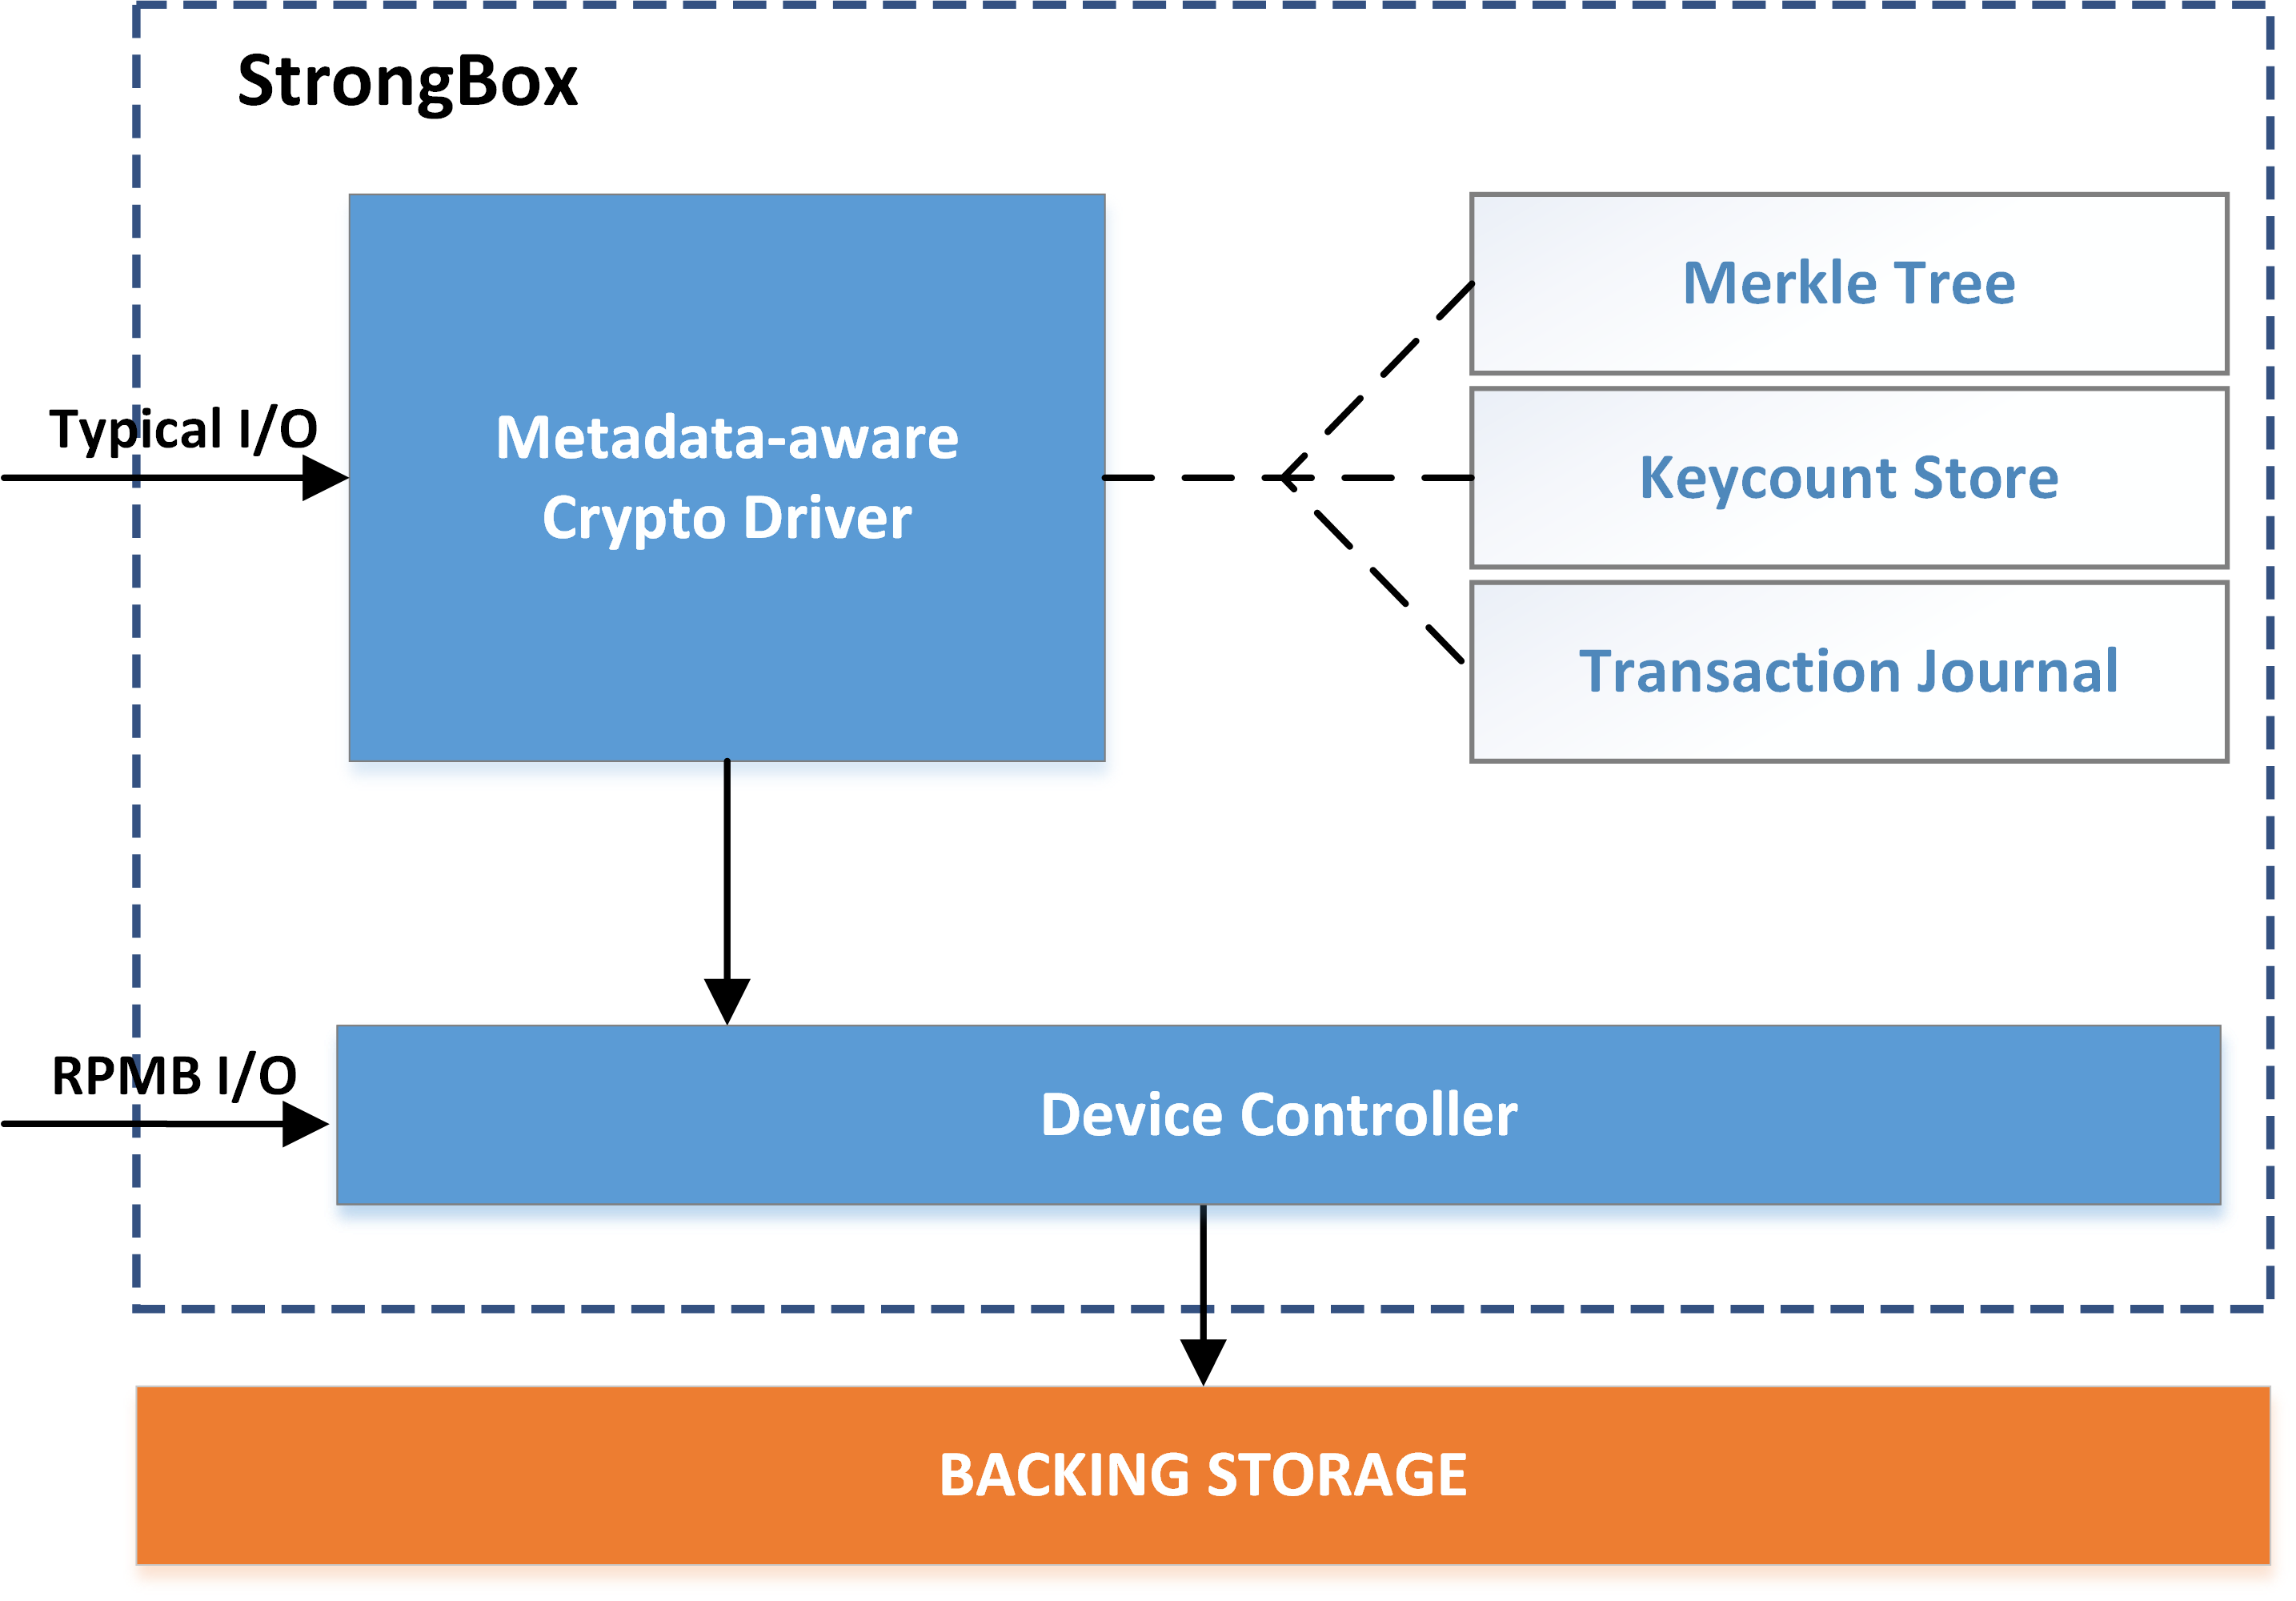
\includegraphics[width=\linewidth]{figs/sc/overview.png}
   \caption{Overview of the SwitchCrypt construction.} \label{fig:overview}
\end{figure}

SwitchCrypt consists of a \emph{Generic Stream Cipher Interface} and
\emph{Cryptographic Driver} and sits between a Log-structured File System (LFS)
on the OS, and the underlying drive (backing storage) and device controller
(e.g. Flash Translation Layer). This is illustrated in \figref{overview}, which
provides an overview of the SwitchCrypt system design.

\begin{figure}[t]
   \centering
   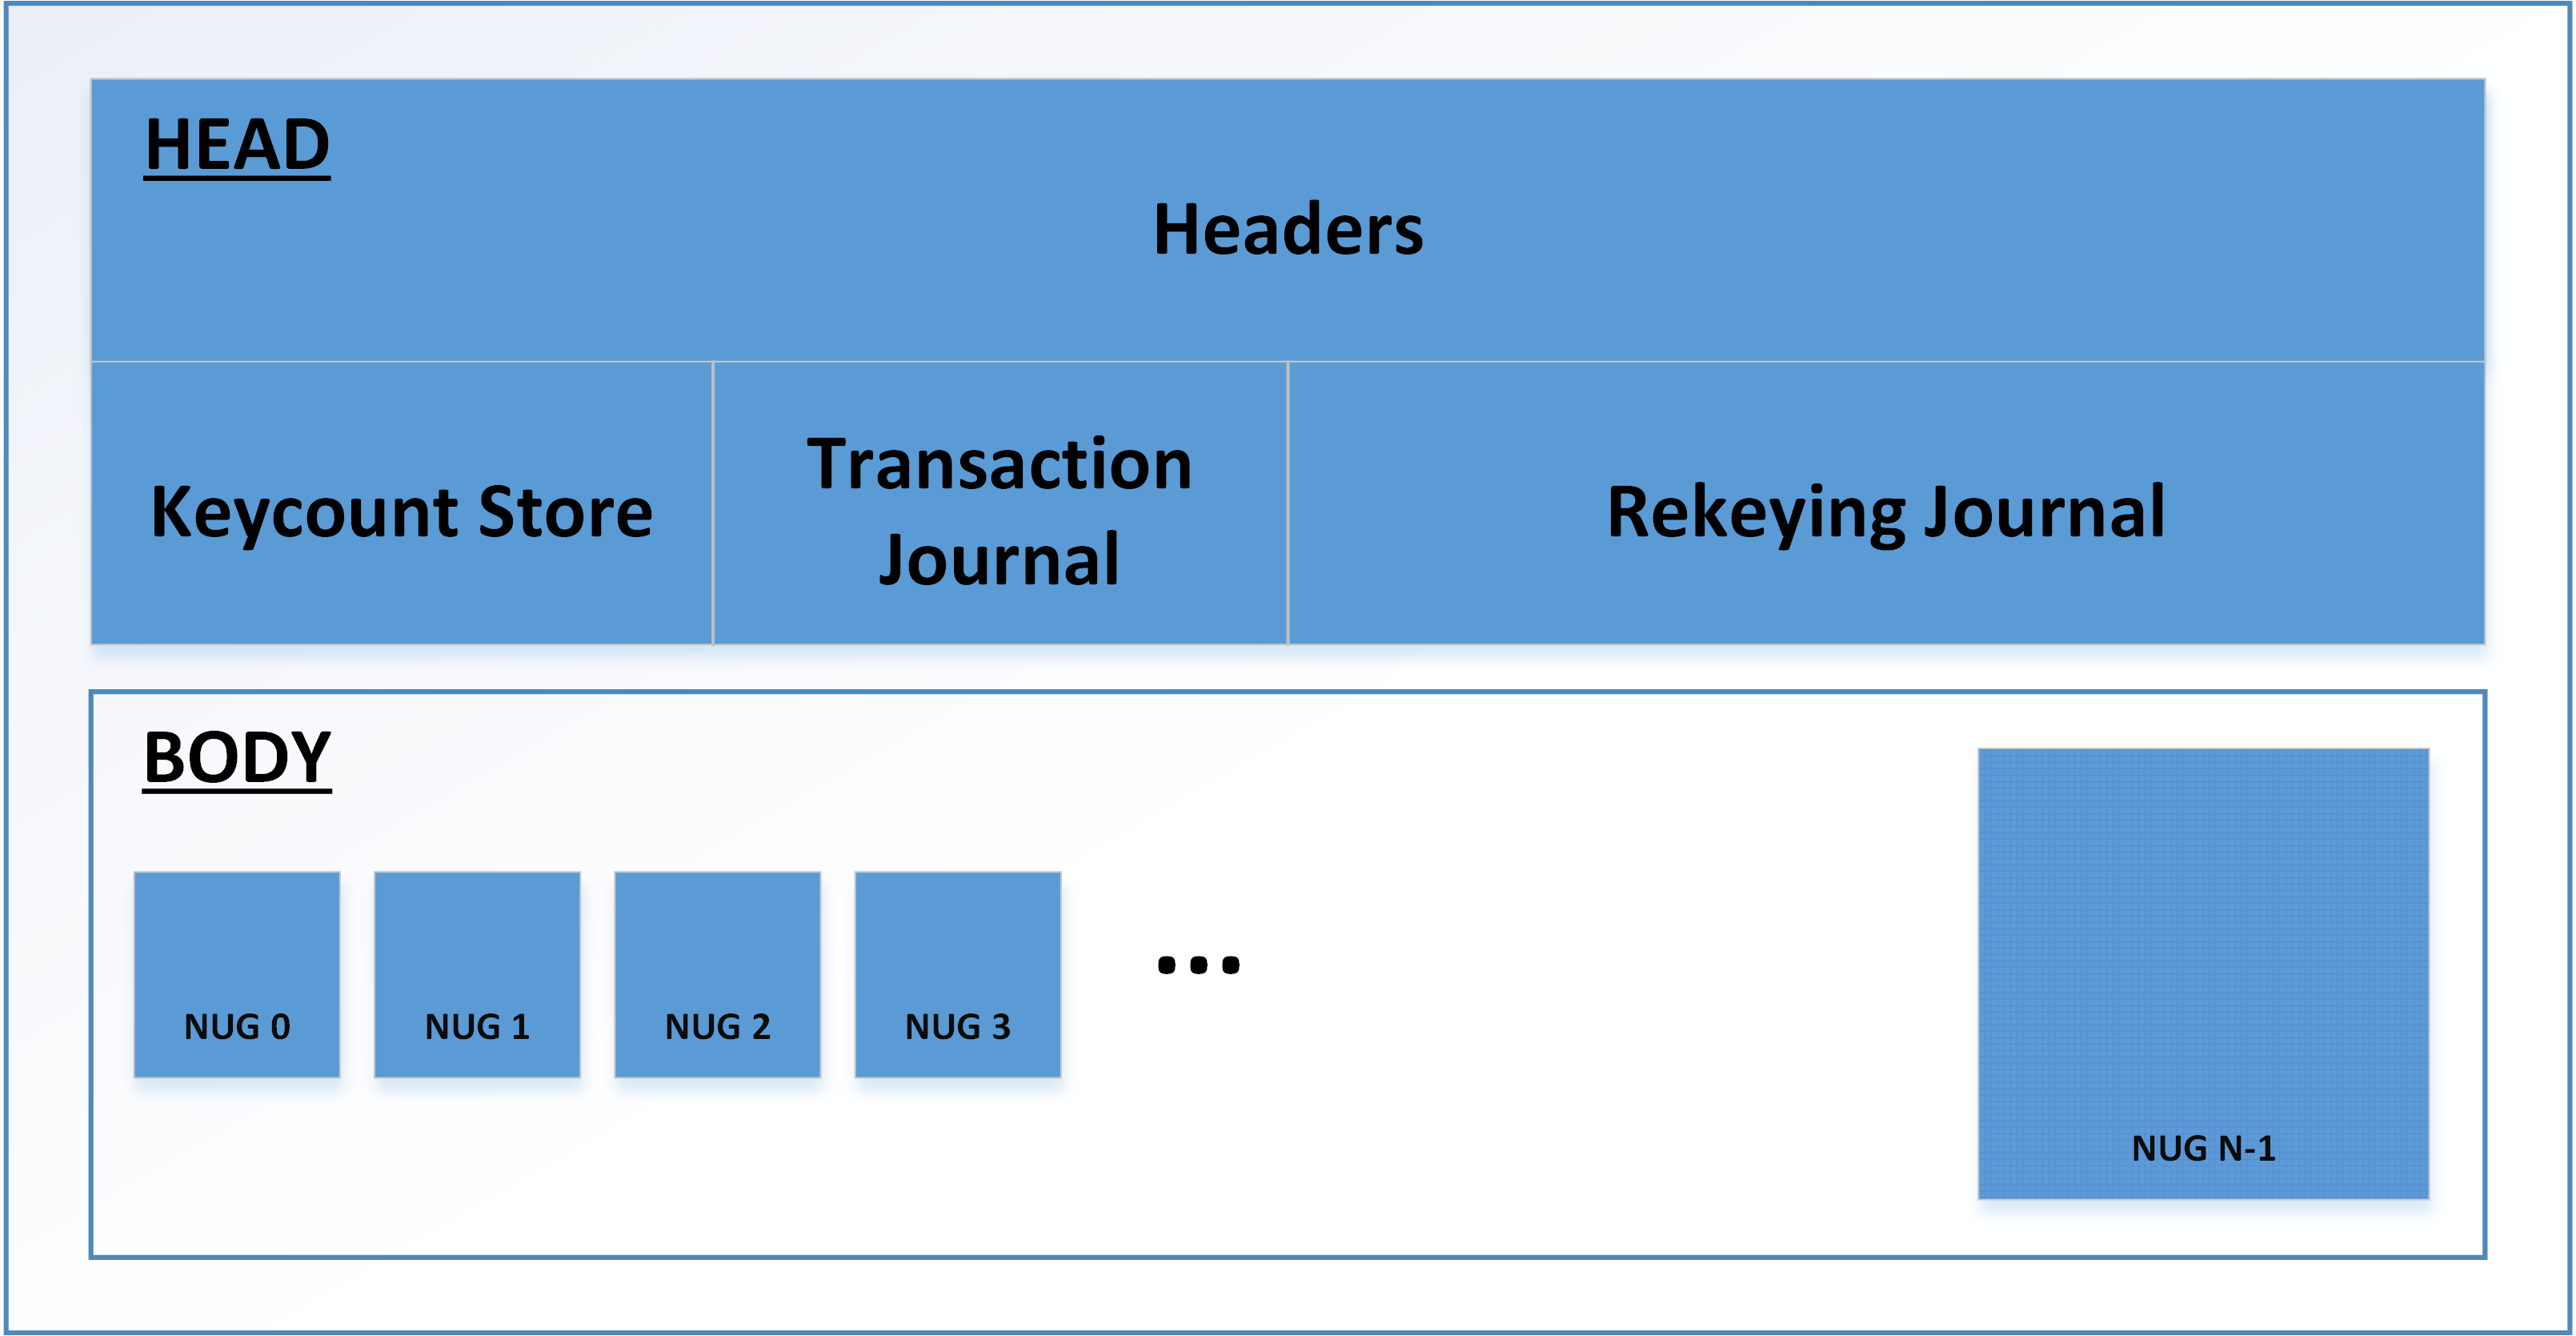
\includegraphics[width=\linewidth]{figs/sc/backstore.png}
   \caption{Layout of SwitchCrypt's drive layout.} \label{fig:backstore}
\end{figure}

The drive itself is divided into a \emph{HEAD} section and \emph{BODY} section
upon initialization, illustrated in \figref{backstore}. The HEAD consists of
metadata headers written during initialization~\cite{StrongBox} along with the
\emph{Keycount Store}, \emph{Transaction Journal}, \emph{Rekeying Journal}, and
\emph{Per-Nugget Metadata}, each drive-backed. These components are used by the
\emph{Cryptographic Driver} together with the \emph{Cipher Switching Strategy}
implementations to enable efficient per-unit cipher switching.

The BODY consists of a series independent same-size logical units called
\emph{nuggets}. A nugget consists of one or more contiguous physical drive
blocks. Each nugget is coupled with metadata in the HEAD indicating which cipher
was used to encrypt the nugget along with any additional ciphertext output; the
latter allows us to treat any non-length-preserving ciphers as if they were
length-preserving. SwitchCrypt uses the Keycount Store and Transaction Journal
components along with our nugget layout to 1) track, detect, and handle
overwrites, 2) limit the maximum length of any plaintext input to ciphers, thus
amortizing the overhead incurred during encryption, and 3) independently and
efficiently switch the cipher used to encrypt individual nuggets.

StrongBox demonstrated how to make nugget-based drive organization secure using
a single stream cipher, ChaCha20, to handle overwrites, prevent rollback
attacks, and limit plaintext length~\cite{StrongBox}. However, StrongBox's was
not designed envisioning the utility in trading off between concerns at the
filesystem or device-mapper level, dynamic cipher switching, or protecting
against attacks on data ``in motion;'' the remainder of this section details the
novel components that enable this functionality. Specifically: how we quantify
the properties traded off between configurations (\cref{subsec:quantify}), the
Generic Stream Cipher Interface and Per-Nugget Metadata components
(\cref{subsec:interface}) which decouple cipher implementations from the
encryption process, and our Cipher Switching Strategy implementations
(\cref{subsec:strategies}) used to efficiently encrypt nuggets with different
ciphers.

\subsection{Quantifying Cipher Security Properties} \label{subsec:quantify}

To reason about when to trade off between the ciphers evaluated in this work, we
must have a way to compare ciphers' utility in the context of SwitchCrypt FDE.
However, different ciphers have a wide range of security properties, performance
profiles, and output characteristics. To address this need, we propose a novel
evaluation framework (see: \tblref{security-quant}). Our framework classifies
stream ciphers according to three quantitative features: relative round count,
ciphertext randomization, and ciphertext expansion. Taken together, these
features reveal a rich tradeoff space of cipher configurations optimizing for
different combinations of concerns.

\begin{table}[ht]
   \centering
   \begin{tabular}{@{}ccccc@{}}
   \toprule
   \textbf{Cipher} & \textbf{Rounds} & \textbf{Randomization} &
   \textbf{Expansion} \\
   \midrule
   ChaCha8         & 0           & 0           & 1           \\
   ChaCha12        & 0.5         & 0           & 1           \\
   ChaCha20        & 1           & 0           & 1           \\
   Salsa8          & 0           & 0           & 1           \\
   Salsa12         & 0.5         & 0           & 1           \\
   Salsa20         & 1           & 0           & 1           \\
   HC128           & 0           & 0           & 1           \\
   HC256           & 1           & 0           & 1           \\
   Freestyle (F)   & 0           & 2           & 0           \\
   Freestyle (B)   & 0.5         & 2.5         & 0           \\
   Freestyle (S)   & 1           & 3           & 0           \\
\end{tabular}
   \caption{Our framework for classifying stream ciphers according to three
   ideal features: relative round count, ciphertext randomization, and
   ciphertext expansion.}
   \label{tbl:security-quant}
 \end{table}

\subsubsection{Relative Rounds (Rounds)}

The ciphers we examine in this work are all constructed around the notion of
\emph{rounds}, where a higher number of rounds (and possibly longer key) is
positively correlated with a higher resistance to brute force given no fatal
related-key or other attacks~\cite{ChaCha-Cryptanalysis}. Hence, this feature
represents how many rounds a cipher executes relative to other implementations
of the same algorithm. For instance: ChaCha8 is a reduced-round version of
ChaCha12, which is a reduced-round version of ChaCha20, all using the ChaCha
algorithm~\cite{ChaCha20,ChaCha-Cryptanalysis}.

We limit our analysis to groups of three implementations, each using a different
number of rounds. In the case of HC-128 and HC-256, we limit our analysis to a
group of two implementations. Scores range from 0 (least number of rounds
considered) to 1 (greatest number of rounds considered).

\subsubsection{Ciphertext Randomization (Randomization)}

A cipher with ciphertext randomization generates different ciphertexts
non-deterministically given the same key, nonce, and plaintext. This makes it
much more difficult to execute chosen-ciphertext attacks (CCA), key
re-installation attacks, XOR-based cryptanalysis and other comparison attacks,
and other confidentiality-violating schemes where the ciphertext is in full
control of the adversary ~\cite{Freestyle}. This property is useful in cases
where we cannot prevent the same key, nonce, and plaintext from being reused,
such as with data ``in motion'' (see the motivational example in
\secref{sc-motivation}). Ciphers without this property---such as ChaCha20 on
which prior work is based---are trivially broken when key-nonce-plaintext
3-tuples are reused. In StrongBox, this is referred to as an ``overwrite
condition'' or simply ``overwrite''~\cite{StrongBox}.

Though there are many ways to achieve ciphertext randomization, the ciphers
included in our analysis implement it using a random number of rounds for each
block of the message where the exact number of rounds are unknown to the
receiver a priori~\cite{Freestyle}. In determining the minimum and maximum
number of rounds used per block in this non-deterministic mode of operation, we
can customize the computational burden an attacker must bear by choosing lower
or higher minimums and maximums. Hence, this is not a binary feature; scores
range from 0 (no ciphertext randomization) to 1 (lowest minimum and maximum
rounds per block) to 3 (highest minimum and maximum rounds per block).

\subsubsection{Ciphertext Expansion (Expansion)}

A cipher that exhibits ciphertext expansion is non-length-preserving: it outputs
more or less ciphertext than was originally input as plaintext. This can cause
major problems in the FDE context. For instance, cryptosystems that rely on
AES-XTS (e.g. Linux's dm-crypt, Microsoft's BitLocker, Apple's FileVault) or
ChaCha (e.g. StrongBox, Google's Adiantum) have storage layouts that hold
length-preserving output as an invariant, making ciphers that do not exhibit
this property incompatible with their implementations; yet, ciphertext expansion
is often (but not always) a necessary side-effect of ciphertext randomization.

The ciphers included in our analysis that exhibit ciphertext expansion have an
overhead of around 1.56\% per plaintext message block~\cite{Freestyle}. Even a
single byte of additional ciphertext vs plaintext would make a cipher
inappropriate for use with prior work. Hence, this is a binary feature in that a
cipher either outputs ciphertext of the same length as its plaintext input or it
does not. A cipher scores either a 0 if it \emph{is not} length-preserving in
this way or a 1 if the ciphertext is always the same length as the plaintext.

\subsection{Generic Stream Cipher Interface} \label{subsec:interface}

One of the goals of SwitchCrypt is that we might use any stream cipher
regardless of its implementation details. Yet this is entirely non-trivial.
There are many cipher implementations that we might use with SwitchCrypt, each
with unique input requirements and output considerations. For instance, Salsa
and Chacha implementations require a certain IV and key size and handle
plaintext input through successive invocations of a single state update
function~\cite{Floodyberry}. Using OpenSSL's AES implementation in CTR mode
requires manually tracking the counter state and individual ciphertext blocks
are retrieved though corresponding function invocations. Freestyle's reference
implementation requires we calculate the extra space necessary per nugget (due
to ciphertext expansion) along with configuration-dependent minimum and maximum
rounds-per-block, hash interval, and pepper bits~\cite{Freestyle}. HC-128 and
other ciphers have similarly disparate requirements.

Unlike prior work, SwitchCrypt must be able to encrypt and decrypt arbitrary
nuggets \emph{with any of these ciphers} at any moment with low overhead and
without tight coupling to any specific implementation detail. Hence, there is a
need for an interface that completely decouples cipher implementations from the
encryption/decryption process. Our novel cipher interface allows any stream
cipher to be integrated into SwitchCrypt without modifications to third-party
code, enabling normally incompatible ciphers to encrypt and decrypt arbitrary
nuggets. The ability for disparate cipher implementations to co-exist forms the
foundation for SwitchCrypt's ability to switch the system between different
cipher configurations in our tradeoff space efficiently and effectively.

To facilitate this, the Generic Stream Cipher Interface presents the
cryptographic driver with a single unified encryption/decryption model.
SwitchCrypt receives I/O requests from the operating system at the block device
level like any other device-mapper. These requests come in the form of either
reads or writes. When a read request is received, the OS hands SwitchCrypt an
offset and a length and expects a response with plaintext of that specific
length starting at that specific offset taken from the beginning of storage
(i.e. the BODY section; see \figref{backstore}). When a write request is
received, the OS hands SwitchCrypt an offset, a length, and a buffer of
plaintext and expects that plaintext to be encrypted and committed to storage
such that the plaintext is later retrievable given that same offset and length
in a future read request. These requests can either be handled together by a
single function or handled individually as distinct read and write operations,
each with different tradeoffs.

\begin{enumerate}
   \item \textbf{\texttt{xor\_interface}}\\\texttt{xor\_interface} executes
   independently of SwitchCrypt internals and treats encryption and decryption
   as the same operation. Implementations receive an integer offset $F$, an
   integer length $L$, a key buffer $K$ corresponding to the current nugget, and
   an empty $L$-length XOR buffer. SwitchCrypt expects the XOR buffer to be
   populated with $L$ bytes of keystream output from some stream cipher seeked
   to offset $F$ with respect to key $K$. The length of the key buffer will
   always be exactly what the cipher implementation expects, alleviating the
   burden of key management; similarly, the XOR buffer will be XOR-ed with the
   appropriate portion of nugget contents automatically, alleviating the burden
   of drive access and other tedious calculations. \\
   \item \textbf{\texttt{read\_interface}} and
   \textbf{\texttt{write\_interface}}\\
   Unlike \texttt{xor\_interface}, encryption and decryption are distinct
   concerns at this abstraction level. \\\texttt{read\_interface} handles
   decryption during reads. \\\texttt{write\_interface} handles encryption
   during writes. Implementations receive full access to SwitchCrypt internals,
   giving wrapper code complete control over the encryption and decryption
   process and allowing implementers to bypass parts of the nugget-based drive
   layout abstraction (i.e. BODY) if necessary. This comes at the cost of 1)
   significantly increased code complexity, as the implementer must perform
   certain I/O manually, distinguish between independent nuggets on the drive,
   determine what to encrypt or decrypt at what offset and when, when to commit
   which metadata and where and 2) potential performance implications, since
   SwitchCrypt must account for not having absolute control over its internal
   data structures during function invocation. For a cipher like Freestyle,
   configurations with lower minimum and maximum rounds per block may see a
   performance improvement here, while configurations with higher minimum and
   maximum rounds per block may see reduced performance.
\end{enumerate}

\subsection{Cipher Switching Strategies} \label{subsec:strategies}

The Generic Stream Cipher Interface allows many differently ciphered nuggets to
co-exist on the same drive. However, at any moment, there is only a single
\emph{active cipher configuration} (henceforth \emph{active configuration}). The
active configuration is used to encrypt nugget contents. When a cipher switch is
triggered, a different configuration becomes the active configuration. At this
point, SwitchCrypt must determine \emph{when} to re-cipher a nugget and
\emph{where} to store the output on the drive. ``Re-ciphering'' here means using
an inactive configuration to decrypt a nugget's contents and using the active
configuration to re-cipher it. Depending on the use case, it may make the most
sense to re-cipher a nugget immediately, or eventually, or to maintain several
areas of differently-ciphered nuggets concurrently.

A naive approach would switch every nugget in BODY to the active configuration
immediately, but the latency and energy cost would be unacceptable. Hence, a
more strategic approach is necessary. We satisfy this need with our \emph{cipher
switching strategies}. These novel strategies allow for nuggets to be
re-ciphered in a variety of cases with minimal impact on performance and battery
life and without compromising security. This is thanks to the nugget-based drive
layout, which limits the churn of cipher switching operations to relatively
small regions of ciphertext on the drive.

Determining \emph{when} to target a nugget for re-ciphering we call
\emph{temporal switching}, for which we propose the \emph{Forward} switching
strategy. Determining \emph{where}---in which storage region and across which
nuggets---to output ciphertext we call \emph{spatial switching}, for which we
propose the \emph{Mirrored} and \emph{Selective} switching strategies. \\

\textbf{Forward Switching Strategy.} When a nugget is encountered during I/O
that was encrypted using something other than the active configuration, the
Forward strategy dictates that this nugget be re-ciphered immediately. If a
particular nugget encrypted with an inactive configuration is never encountered
during I/O, it is never re-ciphered and remains on the drive in its original
state. In this way, the Forward strategy represents a form of temporal cipher
switching.

Rather than re-cipher the entire drive every time the active configuration
changes, this strategy limits the performance impact of cipher switching to
individual nuggets. The expense of re-ciphering is paid only once, after which
the nugget is accessed normally during I/O until the active configuration is
switched again.

There are several forms the Forward strategy might take. The default and
most intuitive is \emph{0-forward}, in which SwitchCrypt immediately transitions
individual nuggets encountered during I/O to the active configuration if they
are not using it. Over time, if various I/O operations end up touching every
nugget in the drive, the encrypted contents of every nugget will become
decryptable with the currently active configuration.

The Forward strategy might also take the form of \emph{N-forward}, where
SwitchCrypt attempts to take advantage of spatial sequential locality to
transition whole sets of nuggets into the active configuration. We can trivially
expand the forward strategy to encompass the entire drive by selecting $N$ equal
to the total number of nuggets managed by SwitchCrypt. This would have the
overhead of re-ciphering large swaths of the drive upon every I/O operation
where a nugget encrypted with the inactive configuration is encountered. Of
course, this has the same dire implications for performance as simply
re-initializing the entire system or encrypted container with the new cipher. \\

\textbf{Selective Switching Strategy.} When SwitchCrypt is initialized with the
Selective strategy, the drive is partitioned into $C$ regions where $C$
represents the total number of available ciphers in the system; each regions'
nuggets are encrypted by each of the $C$ ciphers respectively. For instance,
were SwitchCrypt initialized using two ciphers ($C = 2$), the drive would be
partitioned in half; all nuggets in the first region would be encrypted with the
first cipher while all nuggets in the second would be encrypted with the other.


When using this strategy, the active cipher determines which partition we
``select'' for I/O operations. Hence, unlike the Forward strategy, which
schedules individual nuggets to be re-ciphered at some point in time after the
active configuration is switched, the Selective strategy allows the wider system
to indicate \emph{where} on the drive a read or write operation should occur. In
this way, the Selective strategy represents a form of spatial cipher switching
where different regions of the drive can store differently-ciphered nuggets
independently and concurrently. A user could take advantage of this to, for
instance, set up regions with different security properties and performance
characteristics, managing them as distinct virtual drives or transparently
reading/writing bytes to different security regions on the same drive. \\

\textbf{Mirrored Switching Strategy.} Similar to the Selective strategy, when
SwitchCrypt is initialized with the Mirrored strategy, the drive is partitioned
into $C$ regions where $C$ represents the total number of available ciphers in
the system; each regions' nuggets are encrypted by each of the $C$ ciphers
respectively.

However, unlike the Selective strategy, all write operations that hit one region
are mirrored into the other regions immediately, so all regions of the drive
will always be in a consistent state and always share the same data. The active
configuration determines \emph{where} a read operation should occur. In this
way, the Mirrored strategy represents a form of spatial cipher switching because
we are switching which configuration we are using to read in data. A user could
take advantage of this along with SSD Instant Secure Erase~\cite{ISE1,ISE2,ISE3}
to delete other regions, thus quickly and securely converging the drive to a
single configuration without losing any data or suffering the egregious
performance or battery penalty that comes with re-ciphering every nugget.

\subsubsection{Comparing Cipher Switching Strategies}

\begin{table}[t]
   \centering
   \begin{tabular}{@{}|c|c|c|C{25mm}|@{}}
      \toprule
      \textbf{Strategy} & \textbf{Convergence} & \textbf{Waste} &
      \textbf{Performance} \\
      \midrule
      Forward   & Slower       & None & Faster reads and writes unless switching
      \\\hline
      Mirrored  & Nearly instant & High & Faster reads; slower writes \\
      \hline
      Selective & Slower       & High & Faster reads and writes  \\
      \hline
   \end{tabular}
   \caption{A summary comparison between the three cipher switching strategies.}
   \label{tbl:strategies-advantages}
\end{table}

\tblref{strategies-advantages} summarizes the higher level tradeoffs between the
three cipher switching strategies.

\textbf{Convergence.} Depending on the use case, the ability to quickly converge
the entire drive to a single cipher configuration without losing data is very
useful (see: \secref{sc-usecases}). The near-instantaneous ``just forget the key''
nature of SSD Instant Secure Erase (ISE) implementations on modern
SSDs~\cite{ISE1,ISE2,ISE3} makes this a very fast process for the Mirrored
strategy. The Forward strategy is slow to converge compared to Mirrored since,
in the worse case, every nugget on the drive will require re-ciphering. The
Selective strategy is similarly slow to converge since entire regions of nuggets
must be moved and re-ciphered to prevent data loss; those regions could be
destroyed without moving data around using ISE too, which would be very fast,
but unlike Mirrored some data would be lost forever.

\textbf{Waste.} Unlike the other two strategies, using the Forward strategy does
not reduce the total usable space on the drive by the end-user, ciphertext
expansion notwithstanding. We refer to this as ``waste''. The Forward strategy
is not wasteful in this way because it allows differently-ciphered nuggets to
co-exist contiguously on the drive without special partitions. Since the
Mirrored and Selective strategies require partitioning the drive into some
number of regions---where the writeable size reported back to the OS is some
function of region size---there is a necessary reduction in usable space.

\textbf{Performance.} The Selective and Mirrored strategies can read data from
the drive with low overhead, reaching performance parity with prior work,
because they never have to deal with on-demand re-ciphering. This is because
switching ciphers using these two strategies amounts to offsetting the read
index so that it lands in the proper BODY partition on the drive, which has
little overhead. The Forward strategy also reads with low overhead except in the
case where a nugget was not encrypted with the active configuration. This
triggers re-ciphering on-demand, which can be costly if the workload constantly
touches unique nuggets and is small enough that cost is not amortized.

The Selective strategy also writes with low overhead because, like with reads,
an index offset is the only requirement. The Mirrored strategy, on the other
hand, can be up to two times slower for writes (when $C = 2$) compared to
baseline. Each additional region ($C > 2$) compounds the write penalty depending
on the workload. This is because each write is mirrored across \emph{all}
regions. As with reads, the Forward strategy writes with low overhead except in
the case where a nugget was not encrypted with the active configuration. This
triggers re-ciphering on-demand, which can be costly if the workload touches
unique nuggets and is small enough that cost is not amortized.\\

With these tradeoffs in mind: Mirrored is ideal when the drive must converge
quickly, write performance is not a primary concern, and drive space is
abundant; Selective is ideal when different data should be encrypted differently
and drive space is abundant; and Forward is ideal when some subset of nuggets
should be encrypted differently without wasting drive space. See
\secref{sc-usecases} for specific scenarios that demonstrate these differences in
practice.

\subsubsection{Threat Model for Cipher Switching Strategies}

The primary concern facing any FDE solution is that of confidentiality. An
adversary should not be able to reveal any information about encrypted plaintext
without the proper key. As with prior work, encryption is achieved via a binary
additive approach: cipher output (keystream) is combined with plaintext nugget
contents using XOR, with metadata to track writes and ensure that pad reuse
never occurs during overwrites and that the system can recover from crashes into
a secure state. Another concern is data integrity: an adversary should not be
able to tamper with ciphertext and it go unnoticed. Nugget integrity is tracked
by an in-memory Merkle tree. See the threat model addressed by Dickens et
al.~\cite{StrongBox} for further details.

Switching strategies add an additional security concern not addressed by prior
work: even if we initiate a ``cipher switch,'' there may still be data on the
drive that was encrypted with an inactive configuration. Is this a problem? For
the Forward strategy, this implies data may at any time be encrypted using the
``least desirable cipher''. For the Mirrored and Selective strategies, the drive
is partitioned into regions where nuggets are guaranteed to be encrypted with
each cipher, including the ``least desirable cipher''. However, in terms of
confidentiality, the confidentiality guarantee of SwitchCrypt can be reduced to
the individual confidentiality guarantees of the available ciphers used to
encrypt nuggets.

\subsection{Putting It All Together} \label{subsec:summary}

We revisit the motivating example from \secref{sc-motivation}, where we are
using Freestyle to ensure secure backups. Initially, I/O requests come down from
the LFS and are received by the cryptographic driver, which divides the request
based on which nuggets it touches. For each nugget, the per-nugget metadata is
consulted to determine with which cipher the nugget is encrypted. If it is
encrypted with the active cipher configuration (Freestyle), which must be true
if we have not initiated a cipher switch, the write is handled similarly to
prior work: encrypted data is read in from the drive, the merkle tree and
monotonic counter are consulted to ensure the integrity of encrypted data, the
transaction journal is consulted during write operations so that overwrites are
handled and pad reuse violations are avoided, and then the keycount store is
consulted to derive the nugget's unique encryption key from some master secret.
Finally, using the Generic Stream Cipher Interface, we call out to the
Freestyle, allowing SwitchCrypt to encrypts/decrypts the nugget's contents and
commit any updates back to storage. All the while, the drive's
Freestyle-encrypted contents are being uploaded up to our enterprise backup
service every so often.

When the device enters ``battery saver'' mode, drive backups are paused, the
energy monitoring software downclocks the CPU, and the OS signals to SwitchCrypt
that a more energy-efficient cipher (ChaCha20) should be used until we return to
a non-curtailed energy budget. SwitchCrypt sets ChaCha20 as the active cipher
configuration. Now, when the cryptographic driver divides I/O requests into each
affected nugget, the per-nugget metadata shows SwitchCrypt that each nugget is
encrypted using a cipher that is not the active configuration. This triggers the
re-ciphering code path. Since we are using the Forward switching strategy in
this example, nugget data is immediately decrypted by calling out to the
inactive configuration through the Generic Stream Cipher Interface, after which
the nugget is re-ciphered by calling out to the active configuration. Finally,
the cryptographic driver manages encrypting/decrypting data and updating the
merkle tree and monotonic counter, transaction journal, and keycount store as
the I/O operation and related metadata is committed to the drive afterwards.

Now, thanks to SwitchCrypt, the system can adapt to changing requirements beyond
the capability of prior work. See \secref{sc-usecases} for specifics.

\section{Implementation} \label{sec:hc-implementation}

We implement a proof-of-concept HASCHK frontend as a Google Chrome extension.
To demonstrate the general applicability of our approach, our frontend currently
works with two backends: (1) directly with DNS via Google's JSON API for DNS
over HTTPS (DoH) and (2) indirectly with DHT (Ring OpenDHT) via a local
Representational State Transfer (REST) API we designed to mimic the response
syntax of Google's DoH JSON API. Other candidate backends include storage
clusters, relational and non-relational databases, and any high availability
key-value store.

Our extension operates following the high level overview in \figref{protocol}
with some key implementation-specific functionality that we explore in the
remainder of this subsection. After the user initiates a download either
directly (\eg{ typing a URI manually}) or by following a hyperlink, our
extension, having observed the initial web request, associates that request with
the new download item. The original request may have directly triggered the
download or the download may have been triggered after one or more redirections.
Our extension derives the correct BD in both cases (see below). At this point,
if the backend does not exist or does not conform to the protocol, the protocol
terminates. Otherwise, after the download completes, a URN is calculated and
combined with the BD to make a final query to the backend. In effect, this query
asks: \emph{is this resource compromised?} If the response to the query is
negative (\ie{ a DNS TXT record or DHT data value}), the extension considers the
resource validated. On the other hand, if the response to the query is positive
(\ie{ no record found or bad data value returned}), the extension considers the
resource compromised, deletes the resource file, and warns the user.

In keeping with UX suggestions of prior work, our extension is virtually
transparent to end users in the common case that a download is successfully
verified by a provider's backend or when HASCHK has not been properly
deployed by a provider. However, in the relatively uncommon case that a resource
is deemed compromised, the extension will delete the file and alert the user
with the primary option to ``dismiss'' the alert, mimicking Chrome's own highly
effective dangerous download warning~\cite{ChromeClickThrough}. Specifically:
the user has the option of clicking through the warning via a low-key secondary
interface where they can force the extension to ignore the compromised nature of
the resource \emph{the next time it is downloaded}, forcing the user to trigger
the download again. This inconvenience, favoring users' security over choice, is
in keeping with the recommendations of prior work regarding security warning UX
(see \secref{hc-motivation}).

As no JavaScript OpenDHT client implementation exists, we developed a REST API
to facilitate communication between our extension and the Ring OpenDHT network
via HTTP and JSON. In a production implementation, a JavaScript OpenDHT client
would be baked directly into the extension.

Deploying the DNS backend is as simple as adding certain TXT records to our DNS
zone. This is a straightforward operation. Similarly, deploying the DHT backend
requires adding certain key-value pairs to the OpenDHT network, which is
trivial. Moreover, both DNS and DHT backends are performant and highly
available. The Ring OpenDHT network is also free to use. In the case of DNS, the
vast majority of web-facing providers and IT teams are already using it, already
pay for their own DNS zones, and are already quite familiar with configuring and
managing them. Hence, no exotic secondary backend system is required for
providers with web servers. Additionally, we argue updating the URNs stored by
these backends automatically---by integrating a URN calculation and record
insertion/update step into a modern development toolchain or resource deployment
pipeline---is relatively low-effort and straightforward for providers.

No application or website source code changes, costly user-facing server or web
infrastructure customizations, or modifications to web standards are needed to
enable our extension to protect a provider's resources. Given a production-ready
implementation of our frontend---coupled with the near ubiquitous adoption of
DNS---HASCHK (with a DNS backend) could be deployed immediately by interested
providers.

\subsection{URNs, BDs, and Fallthrough in Google Chrome}

BD derivation in the browser is non-trivial. Users can initiate downloads
through clicking links inside \emph{and outside} the browser (\eg{ in an email
application}), through asynchronous JavaScript, and by entering URIs into the
browser manually. To catch these and other edge cases, we implement our
extension using the WebRequest API~\cite{ExtensionAPI}, which allows us to
monitor all navigation events, collate redirects into an interrogable chain of
requests, and associate new download items with the URI where they were
originally initiated.

To query the backend, we: (1) BASE32 encode the resource's URN. (2) Divide the
112-character result into two 56-character strings \texttt{C1} and \texttt{C2}.
(3) We calculate the BD, which is either the 3LD and 2LD from
\texttt{details.originUrl}. We choose by issuing up to two queries of the form
\texttt{AL.BD}, where the Application Label (AL) is the constant string
\texttt{\_haschk}, looking for a response containing the value \texttt{OK}. We
first query the 3LD as BD and, if we do not receive the proper response there,
query the 2LD as BD. If the proper response is not received from either query,
the extension assumes HASCHK has not been properly deployed and terminates.
(4) Otherwise, concatenating C1, C2, AL, and BD, we issue a query of the form
\texttt{C1.C2.AL.BD}, again looking for a response containing \texttt{OK}
(negative) or that the query was not found (positive).

To handle redirection, we use Chrome's Web Request API to associate redirected
requests with one another. The originating request's \texttt{origin} at the top
of this chain is used to derive the BD using the \texttt{details.originUrl} and
\texttt{details.documentUrl} properties (also avoiding iframe issues). This
prevents an adversary from trivially fooling HASCHK by replacing a legitimate
hyperlink with a malicious one. A naive implementation might use the
\texttt{DownloadItem.referrer} property to derive the BD, since it should be
populated with the originating URL. Unfortunately, this property can be
manipulated with one or more redirections causing the BD to point into the
attacker's DNS zone. If the attacker properly deploys a HASCHK backend, they
could then trivially force false negatives.

Keeping a chain of associated requests also allows us to implement
``fallthrough'' functionality where, if the original request at the head of the
chain has not deployed HASCHK, the extension can walk the chain, checking
each point of redirection for a proper HASCHK deployment. This ensures URL
shorteners and other redirection services do not trigger false positives.

\section{Evaluation} \label{sec:sc-evaluation}

We implement SwitchCrypt and our experiments on a Hardkernel Odroid XU3 ARM
big.LITTLE system with Samsung Exynos 5422 A15/A7 heterogeneous multi-processing
quad core CPUs at maximum clock speed, 2 gigabyte LPDDR3 RAM at 933 MHz, and an
eMMC5.0 HS400 backing store running Ubuntu Trusty 14.04.6 LTS, kernel version
3.10.106. Energy monitoring was provided by the Odroid's integrated INA-231
power sensors polled every $\approx{260}$ milliseconds (not including
noise/overhead).

We evaluate SwitchCrypt using a Linux RAM disk (tmpfs). The maximum theoretical
memory bandwidth for this Odroid model is 14.9GB/s\@. Our observed maximum
memory bandwidth is 4.5GB/s. Using a RAM disk focuses the evaluation on the
performance differences due to different ciphers.

In each experiment below, we evaluate SwitchCrypt on two high level workloads:
sequential and random I/O. In both workloads, a number of bytes are written and
then read (either 4KB, 512KB, 5MB, 40MB) 10 times. Each workload is repeated
three times for a total of 240 tests per cipher (720 runs per cipher
pair/ratios, explained below); 30 results per byte size, 120 results per
workload. Results are accumulated and the median is taken for each byte size.

When evaluating switching strategies, a finer breakdown in workloads is made
using a pre-selected pair of ciphers we call the \emph{primary cipher
configuration} and \emph{secondary cipher configuration}. SwitchCrypt is
initialized at the primary configuration. Once we trigger a cipher switch,
SwitchCrypt moves towards the secondary configuration via switching strategy.

The cipher switch is triggered according to a certain \emph{ratio} of I/O
operations. For example: given 10 40MB read-write operations, we may write and
then read back 40MB 3 times using the primary cipher, initiate a cipher switch,
and then write and then read back (write-read) 40MB 7 times. This would be a 3:7
ratio. It follows that there are three ratios we use to evaluate SwitchCrypt's
performance in this regard: 7:3, 5:5, and 3:7. Respectively, that is 7 file
write-read operation in the primary cipher for every 3 file write-read
operations in the secondary cipher (7:3), 7 file write-read operation in the
primary cipher for every other file write-read operation in the secondary cipher
(5:5), and 3 file write-read operations in the primary cipher for every 7 file
write-read operation in the secondary cipher (3:7).

All experiments are performed with basic Linux I/O commands, bypassing system
caching.

In this section we answer the following questions:

\begin{enumerate}
 \item What shape does the cipher configuration tradeoff space take under our
 workloads? (\cref{subsec:1})
 \item Can SwitchCrypt achieve dynamic security/energy tradeoffs by reaching
 configuration points not accessible with prior work? (\cref{subsec:2})
 \item What is the performance and storage overhead of each cipher switching
 strategy? (\cref{subsec:3})
\end{enumerate}

\subsection{Switching Strategies Under Various Workloads} \label{subsec:1}

\begin{figure}[ht]
  \textbf{Baseline Cipher I/O Performance}\par\medskip
  {\begin{tikzpicture}[baseline]

    \pgfmathsetmacro{\ymax}{1.1} % set the maximum y value
    \pgfmathsetmacro{\ymaxbreak}{1.2} % set the y value at which overflow is drawn

    \begin{groupplot}[
        group style={
            group size=2 by 2,
            xlabels at=edge bottom,
            ylabels at=edge left,
            xticklabels at=edge bottom,
            yticklabels at=edge left,
            vertical sep=25pt,
            horizontal sep=15pt,
        },
        %axis x line*=bottom,
        height=3.5cm,
        width=\linewidth/1.75,
        tick align=outside,
        tick pos=bottom, % make sure ticks only appear at the bottom and left axes
        title style={yshift=-1.5ex},
        tick style={ black },
        y tick label style={ /pgf/number format/fixed, /pgf/number format/precision=0 },
        grid style={ dotted, gray },
        scatter,
        point meta=explicit symbolic,
        scatter/classes={
            c8={mark=square*},
            c20={mark=triangle*},
            ff={mark=diamond*},
            fb={mark=pentagon*},
            fs={mark=otimes}
        },
        %every node near coord/.append style={font=\tiny},
        %
        % magic to make the numbers appear above the overly long bars:
        % visualization depends on={rawy \as \rawy}, % save original y values
        % restrict y to domain*={ % now clip/restrict any y value to ymax
        %     \pgfkeysvalueof{/pgfplots/ymin}:\ymaxbreak
        % },
        % after end axis/.code={ % draw squiggly line indicating break
        %     \draw [semithick, white, decoration={snake,amplitude=0.1mm,segment length=0.75mm,post length=0.375mm}, decorate] (rel axis cs:0,1.01) -- (rel axis cs:1,1.01);
        % },
        % nodes near coords={\color{.!75!black}\pgfmathprintnumber\rawy}, % print the original y values (darkened in case they are too light)...
        % nodes near coords greater equal only=\ymax, % ... but ONLY if they are >= ymax
        % clip=false, % allow clip to protrude beyond ymax
        % Custom stuff to edit per template
        %
        xlabel={\footnotesize Security Score},
        xlabel near ticks,
        %xlabel shift={-1.5mm},
        xmin=0, xmax=4,
        xtick={ 0, 1, 2, 3, 4 },
        xticklabels={ 0,,, 3, \empty },
        %major x tick style=transparent,
        %enlarge x limits=0.2, % add some breathing room along the x axis's sides
        %
        ylabel={\footnotesize Latency (normalized)},
        ylabel near ticks,
        ylabel shift={-1.5mm},
        ymajorgrids=true,
        ymin=0, ymax=\ymax,
        ytick={ 0, 1, \ymax },
        yticklabels={ 0, 1, \empty },
        %yticklabels={ 0, 0.5, 1.5, 2 },
        % extra y ticks={1},
        % extra y tick style={grid=major, grid style={dashed, black}},
        % extra y tick label={\empty},
        %bar width=4.5pt, % change size of bars
        %
        legend cell align=center,
        legend style={ column sep=1ex },
        legend entries={%
            {\scriptsize 4K},
            {\scriptsize 512K},
            {\scriptsize 5M},
            {\scriptsize 40M}
        },
        legend style={
            draw=none,
            legend columns=4,
            at={(1.0,1.35)},
            anchor=south,
        },
    ]
        \nextgroupplot[title={Sequential Reads}]
            \addlegendimage{no markers,red}
            \addlegendimage{no markers,green,dashed}
            \addlegendimage{no markers,blue,dashdotted}
            \addlegendimage{no markers,orange,densely dotted}
            \addplot [thick, red] table [
                meta=cipher,
                x=score,
                y=latency,
                discard if symbol not={iop}{4k-r},
                discard if symbol not={order}{seq},
                col sep=space,
            ] {data/sc/tradeoff-baseline.dat};
            % \label[c8]{fig:tnr:c8}
            % \label[c20]{fig:tnr:c20}
            % \label[ff]{fig:tnr:ff}
            % \label[fb]{fig:tnr:fb}
            % \label[fs]{fig:tnr:fs}
            \addplot [thick, dashed, green] table [
                meta=cipher,
                x=score,
                y=latency,
                discard if symbol not={iop}{512k-r},
                discard if symbol not={order}{seq},
                col sep=space
            ] {data/sc/tradeoff-baseline.dat};
            \addplot [thick, dashdotted, blue] table [
                meta=cipher,
                x=score,
                y=latency,
                discard if symbol not={iop}{5m-r},
                discard if symbol not={order}{seq},
                col sep=space
            ] {data/sc/tradeoff-baseline.dat};
            \addplot [thick, densely dotted, orange] table [
                meta=cipher,
                x=score,
                y=latency,
                discard if symbol not={iop}{40m-r},
                discard if symbol not={order}{seq},
                col sep=space
            ] {data/sc/tradeoff-baseline.dat};
        \nextgroupplot[legend to name={throwaway1}, title={Random Reads}]
            \addplot [thick, red] table [
                meta=cipher,
                x=score,
                y=latency,
                discard if symbol not={iop}{4k-r},
                discard if symbol not={order}{rnd},
                col sep=space,
            ] {data/sc/tradeoff-baseline.dat};
            \addplot [thick, dashed, green] table [
                meta=cipher,
                x=score,
                y=latency,
                discard if symbol not={iop}{512k-r},
                discard if symbol not={order}{rnd},
                col sep=space
            ] {data/sc/tradeoff-baseline.dat};
            \addplot [thick, dashdotted, blue] table [
                meta=cipher,
                x=score,
                y=latency,
                discard if symbol not={iop}{5m-r},
                discard if symbol not={order}{rnd},
                col sep=space
            ] {data/sc/tradeoff-baseline.dat};
            \addplot [thick, densely dotted, orange] table [
                meta=cipher,
                x=score,
                y=latency,
                discard if symbol not={iop}{40m-r},
                discard if symbol not={order}{rnd},
                col sep=space
            ] {data/sc/tradeoff-baseline.dat};
        \nextgroupplot[legend to name={throwaway2}, title={Sequential Writes}]
            \addplot [thick, red] table [
                meta=cipher,
                x=score,
                y=latency,
                discard if symbol not={iop}{4k-w},
                discard if symbol not={order}{seq},
                col sep=space,
            ] {data/sc/tradeoff-baseline.dat};
            \addplot [thick, dashed, green] table [
                meta=cipher,
                x=score,
                y=latency,
                discard if symbol not={iop}{512k-w},
                discard if symbol not={order}{seq},
                col sep=space
            ] {data/sc/tradeoff-baseline.dat};
            \addplot [thick, dashdotted, blue] table [
                meta=cipher,
                x=score,
                y=latency,
                discard if symbol not={iop}{5m-w},
                discard if symbol not={order}{seq},
                col sep=space
            ] {data/sc/tradeoff-baseline.dat};
            \addplot [thick, densely dotted, orange] table [
                meta=cipher,
                x=score,
                y=latency,
                discard if symbol not={iop}{40m-w},
                discard if symbol not={order}{seq},
                col sep=space
            ] {data/sc/tradeoff-baseline.dat};
        \nextgroupplot[legend to name={throwaway3}, title={Random Writes}]
            \addplot [thick, red] table [
                meta=cipher,
                x=score,
                y=latency,
                discard if symbol not={iop}{4k-w},
                discard if symbol not={order}{rnd},
                col sep=space,
            ] {data/sc/tradeoff-baseline.dat};
            \addplot [thick, dashed, green] table [
                meta=cipher,
                x=score,
                y=latency,
                discard if symbol not={iop}{512k-w},
                discard if symbol not={order}{rnd},
                col sep=space
            ] {data/sc/tradeoff-baseline.dat};
            \addplot [thick, dashdotted, blue] table [
                meta=cipher,
                x=score,
                y=latency,
                discard if symbol not={iop}{5m-w},
                discard if symbol not={order}{rnd},
                col sep=space
            ] {data/sc/tradeoff-baseline.dat};
            \addplot [thick, densely dotted, orange] table [
                meta=cipher,
                x=score,
                y=latency,
                discard if symbol not={iop}{40m-w},
                discard if symbol not={order}{rnd},
                col sep=space
            ] {data/sc/tradeoff-baseline.dat};
    \end{groupplot}%
\end{tikzpicture}%
} \caption{Median sequential and random
  write and then read performance baseline.}
 \label{fig:tradeoff-no-ratios}
\end{figure}

\figref{tradeoff-no-ratios} shows the relative round count, ciphertext
randomization, and ciphertext expansion scores versus median normalized latency
tradeoff between different stream cipher configurations for our sequential and
random I/O workloads. Trends for median hold when looking at tail latencies as
well. Each line represents one workload: 4KB, 512KB, 5MB, and 40MB respectively
(see legend). Each symbol represents one of our ciphers: ChaCha8, ChaCha20,
Freestyle Fast, Freestyle Balanced, and Freestyle Strong. Of the ciphers we
tested, those with higher round counts and higher ciphertext randomization
scores resulted in higher latency and increased energy use for I/O operations.
The relationship between these concerns is not simply linear, however, which
exposes a rich tradeoff space.

Besides the 4KB workload, the shape of each workload follows a similar trend,
hence we will focus on 40MB and 4KB workloads going forward. Due to the overhead
of metadata management and the fast completion time of the 4KB workloads
(\ie{little time for amortization of overhead}), ChaCha8 and ChaCha20 take
longer to complete than Freestyle Fast. This advantage is not enough to make
Freestyle Balanced or Secure workloads complete faster than the ChaCha variants,
however.

Though ChaCha8 is faster than ChaCha20, there is some variability in
our timing setup when capturing extremely fast events occurring close together
in time. This is why ChaCha8 sometimes appears with higher latency than ChaCha20
for normalized 4KB workloads. ChaCha8 is not slower than ChaCha20.

\subsection{Reaching Between Static Configuration Points} \label{subsec:2}

\begin{figure}[ht]
  \textbf{Forward Switching I/O Ratio Performance}\par\medskip
  {\begin{tikzpicture}[baseline]

    \pgfmathsetmacro{\ymax}{1.1} % set the maximum y value
    \pgfmathsetmacro{\ymaxbreak}{1.2} % set the y value at which overflow is drawn

    \begin{groupplot}[
        group style={
            group size=2 by 2,
            xlabels at=edge bottom,
            ylabels at=edge left,
            xticklabels at=edge bottom,
            yticklabels at=edge left,
            vertical sep=25pt,
            horizontal sep=15pt,
        },
        %axis x line*=bottom,
        height=3.5cm,
        width=\linewidth/1.75,
        tick align=outside,
        tick pos=bottom, % make sure ticks only appear at the bottom and left axes
        title style={yshift=-1.5ex},
        tick style={ black },
        y tick label style={ /pgf/number format/fixed, /pgf/number format/precision=0 },
        grid style={ dotted, gray },
        scatter,
        point meta=explicit symbolic,
        scatter/classes={
            c8={mark=square*},
            c20={mark=triangle*},
            ff={mark=diamond*},
            fb={mark=pentagon*},
            fs={mark=otimes}
        },
        %every node near coord/.append style={font=\tiny},
        %
        % magic to make the numbers appear above the overly long bars:
        % visualization depends on={rawy \as \rawy}, % save original y values
        % restrict y to domain*={ % now clip/restrict any y value to ymax
        %     \pgfkeysvalueof{/pgfplots/ymin}:\ymaxbreak
        % },
        % after end axis/.code={ % draw squiggly line indicating break
        %     \draw [semithick, white, decoration={snake,amplitude=0.1mm,segment length=0.75mm,post length=0.375mm}, decorate] (rel axis cs:0,1.01) -- (rel axis cs:1,1.01);
        % },
        % nodes near coords={\color{.!75!black}\pgfmathprintnumber\rawy}, % print the original y values (darkened in case they are too light)...
        % nodes near coords greater equal only=\ymax, % ... but ONLY if they are >= ymax
        % clip=false, % allow clip to protrude beyond ymax
        % Custom stuff to edit per template
        %
        xlabel={\footnotesize R+R (norm)},
        xlabel near ticks,
        %xlabel shift={-1.5mm},
        xmin=0, xmax=4,
        xtick={ 0, 0.5, 1, 2, 3, 4 },
        xticklabels={ ,0,,, 1, \empty },
        %major x tick style=transparent,
        %enlarge x limits=0.2, % add some breathing room along the x axis's sides
        %
        ylabel={\footnotesize Latency},
        ylabel near ticks,
        ylabel shift={-1.5mm},
        ymajorgrids=true,
        ymin=0, ymax=\ymax,
        ytick={ 0, 1, \ymax },
        yticklabels={ 0, 1, \empty },
        %yticklabels={ 0, 0.5, 1.5, 2 },
        % extra y ticks={1},
        % extra y tick style={grid=major, grid style={dashed, black}},
        % extra y tick label={\empty},
        %bar width=4.5pt, % change size of bars
        %
        legend cell align=left,
        legend style={ column sep=1ex },
        legend entries={
            {\scriptsize Baseline},
            {\scriptsize Ratios},
            {\scriptsize },
            {\scriptsize },
            {\scriptsize },
            {\scriptsize C8},
            {\scriptsize C20},
            {\scriptsize FF},
            {\scriptsize FB},
            {\scriptsize FS}
        },
        legend style={
            draw=none,
            legend columns=5,
            at={(1.0,1.35)},
            anchor=south,
        },
    ]
        \nextgroupplot[title={Sequential 40M Reads}]
            \addlegendimage{no markers,red}
            \addlegendimage{mark=otimes*,only marks,black}
            \addlegendimage{only marks,mark=square*,white}
            \addlegendimage{only marks,mark=square*,white}
            \addlegendimage{only marks,mark=square*,white}
            \addlegendimage{only marks,mark=square*,red}
            \addlegendimage{only marks,mark=triangle*,red}
            \addlegendimage{only marks,mark=diamond*,red}
            \addlegendimage{only marks,mark=pentagon*,red}
            \addlegendimage{only marks,mark=otimes,red}
            \addplot [thick, red] table [
                meta=cipher,
                x=score,
                y=latency,
                discard if symbol not={iop}{40m-r},
                discard if number not={ratio}{0},
                discard if symbol not={order}{seq},
                col sep=space,
            ] {data/sc/tradeoff-ratios.dat};
            \addplot [only marks] table [
                x=score,
                y=latency,
                discard if symbol not={iop}{40m-r},
                discard if number not={ratio}{1},
                discard if symbol not={order}{seq},
                col sep=space
            ] {data/sc/tradeoff-ratios.dat};
            \addplot [only marks] table [
                x=score,
                y=latency,
                discard if symbol not={iop}{40m-r},
                discard if number not={ratio}{2},
                discard if symbol not={order}{seq},
                col sep=space
            ] {data/sc/tradeoff-ratios.dat};
            \addplot [only marks] table [
                x=score,
                y=latency,
                discard if symbol not={iop}{40m-r},
                discard if number not={ratio}{3},
                discard if symbol not={order}{seq},
                col sep=space
            ] {data/sc/tradeoff-ratios.dat};
        \nextgroupplot[legend to name={throwaway4}, title={Sequential 4K Reads}]
            \addplot [thick, red] table [
                meta=cipher,
                x=score,
                y=latency,
                discard if symbol not={iop}{4k-r},
                discard if number not={ratio}{0},
                discard if symbol not={order}{seq},
                col sep=space,
            ] {data/sc/tradeoff-ratios.dat};
            \addplot [only marks] table [
                x=score,
                y=latency,
                discard if symbol not={iop}{4k-r},
                discard if number not={ratio}{1},
                discard if symbol not={order}{seq},
                col sep=space
            ] {data/sc/tradeoff-ratios.dat};
            \addplot [only marks] table [
                x=score,
                y=latency,
                discard if symbol not={iop}{4k-r},
                discard if number not={ratio}{2},
                discard if symbol not={order}{seq},
                col sep=space
            ] {data/sc/tradeoff-ratios.dat};
            \addplot [only marks] table [
                x=score,
                y=latency,
                discard if symbol not={iop}{4k-r},
                discard if number not={ratio}{3},
                discard if symbol not={order}{seq},
                col sep=space
            ] {data/sc/tradeoff-ratios.dat};
        \nextgroupplot[legend to name={throwaway5}, title={Sequential 40M Writes}]
            \addplot [thick, red] table [
                meta=cipher,
                x=score,
                y=latency,
                discard if symbol not={iop}{40m-w},
                discard if number not={ratio}{0},
                discard if symbol not={order}{seq},
                col sep=space,
            ] {data/sc/tradeoff-ratios.dat};
            \addplot [only marks] table [
                x=score,
                y=latency,
                discard if symbol not={iop}{40m-w},
                discard if number not={ratio}{1},
                discard if symbol not={order}{seq},
                col sep=space
            ] {data/sc/tradeoff-ratios.dat};
            \addplot [only marks] table [
                x=score,
                y=latency,
                discard if symbol not={iop}{40m-w},
                discard if number not={ratio}{2},
                discard if symbol not={order}{seq},
                col sep=space
            ] {data/sc/tradeoff-ratios.dat};
            \addplot [only marks] table [
                x=score,
                y=latency,
                discard if symbol not={iop}{40m-w},
                discard if number not={ratio}{3},
                discard if symbol not={order}{seq},
                col sep=space
            ] {data/sc/tradeoff-ratios.dat};
        \nextgroupplot[legend to name={throwaway6}, title={Sequential 4K Writes}]
            \addplot [thick, red] table [
                meta=cipher,
                x=score,
                y=latency,
                discard if symbol not={iop}{4k-w},
                discard if number not={ratio}{0},
                discard if symbol not={order}{seq},
                col sep=space,
            ] {data/sc/tradeoff-ratios.dat};
            \addplot [only marks] table [
                x=score,
                y=latency,
                discard if symbol not={iop}{4k-w},
                discard if number not={ratio}{1},
                discard if symbol not={order}{seq},
                col sep=space
            ] {data/sc/tradeoff-ratios.dat};
            \addplot [only marks] table [
                x=score,
                y=latency,
                discard if symbol not={iop}{4k-w},
                discard if number not={ratio}{2},
                discard if symbol not={order}{seq},
                col sep=space
            ] {data/sc/tradeoff-ratios.dat};
            \addplot [only marks] table [
                x=score,
                y=latency,
                discard if symbol not={iop}{4k-w},
                discard if number not={ratio}{3},
                discard if symbol not={order}{seq},
                col sep=space
            ] {data/sc/tradeoff-ratios.dat};
    \end{groupplot}
\end{tikzpicture}%
} \caption{Median sequential and random
  write and then read back performance comparison of Forward switching to
  baseline. Each cluster of 3 dots between configurations represents the 7:3,
  5:5, and 3:7 primary-vs-secondary I/O ratios described in the text.}
 \label{fig:tradeoff-with-ratios}
\end{figure}

\figref{tradeoff-with-ratios} shows the relative round count, ciphertext
randomization, and ciphertext expansion scores versus median normalized latency
tradeoff between different stream ciphers for our sequential and random I/O
workloads with cipher switching using the Forward strategy. After a certain
number of write-read I/O operations, a cipher switch is initiated and
SwitchCrypt begins using the secondary cipher to encrypt and decrypt data. For
each pair of ciphers, this is repeated three times: once at every ratio point
\emph{between} our static configuration points (\ie{7:3, 5:5, and 3:7 described
above}).

The point of this experiment is to determine if SwitchCrypt can effectively
transition the drive between ciphers without devastating performance. For the
40MB, 5MB, and 512KB workloads (40MB is shown), we see that SwitchCrypt can
achieve dynamic security/energy tradeoffs reaching points not accessible with
prior work, all with minimal overhead.

Again, due to the overhead of metadata management for non-Freestyle ciphers (see
\secref{sc-implementation}) and the fast completion time of the 4KB workloads
preventing SwitchCrypt from taking advantage of amortization, ChaCha8 and
ChaCha20 take longer to complete than Freestyle Fast for 4KB reads. We also see
very high latency for ratios between Freestyle Fast and Freestyle Strong cipher
configurations. This is because Freestyle is not length-preserving, so extra
write operations must be performed, and the algorithm itself is generally much
slower than the ChaCha variants (see \figref{tradeoff-no-ratios}). Doubly
invoking Freestyle in a ratio configuration means these penalties are paid more
often.

\begin{figure}[ht]
  \textbf{Mirrored/Selective Switching I/O Ratio Performance}\par\medskip
  \centering
  {\begin{tikzpicture}[baseline]

    \pgfmathsetmacro{\ymax}{1.1} % set the maximum y value
    \pgfmathsetmacro{\ymaxbreak}{1.2} % set the y value at which overflow is drawn

    \begin{groupplot}[
        group style={
            group size=2 by 4,
            xlabels at=edge bottom,
            ylabels at=edge left,
            xticklabels at=edge bottom,
            yticklabels at=edge left,
            vertical sep=25pt,
            horizontal sep=15pt,
        },
        %axis x line*=bottom,
        height=3cm,
        width=\textwidth/4,
        tick align=outside,
        tick pos=bottom, % make sure ticks only appear at the bottom and left axes
        title style={yshift=-1.0ex},
        tick style={ black },
        y tick label style={ /pgf/number format/fixed, /pgf/number format/precision=0 },
        grid style={ dotted, gray },
        scatter,
        point meta=explicit symbolic,
        scatter/classes={
            c8={mark=square*},
            c20={mark=triangle*},
            ff={mark=diamond*},
            fb={mark=pentagon*},
            fs={mark=*},
            mirrored={mark=otimes},
            selective={mark=oplus}
        },
        %every node near coord/.append style={font=\tiny},
        %
        % magic to make the numbers appear above the overly long bars:
        % visualization depends on={rawy \as \rawy}, % save original y values
        % restrict y to domain*={ % now clip/restrict any y value to ymax
        %     \pgfkeysvalueof{/pgfplots/ymin}:\ymaxbreak
        % },
        % after end axis/.code={ % draw squiggly line indicating break
        %     \draw [semithick, white, decoration={snake,amplitude=0.1mm,segment length=0.75mm,post length=0.375mm}, decorate] (rel axis cs:0,1.01) -- (rel axis cs:1,1.01);
        % },
        % nodes near coords={\color{.!75!black}\pgfmathprintnumber\rawy}, % print the original y values (darkened in case they are too light)...
        % nodes near coords greater equal only=\ymax, % ... but ONLY if they are >= ymax
        clip=false, % allow clip to protrude beyond ymax
        % Custom stuff to edit per template
        %
        xlabel near ticks,
        %xlabel shift={-5mm},
        xmin=0, xmax=4,
        %%major x tick style=transparent,
        %enlarge x limits=0.2, % add some breathing room along the x axis's sides
        %
        ylabel={\footnotesize Latency (norm)},
        ylabel near ticks,
        %label shift={-1.5mm},
        ymajorgrids=true,
        ymin=0, ymax=\ymax,
        ytick={ 0, 1, \ymax },
        yticklabels={ 0, 1, \empty },
        %yticklabels={ 0, 0.5, 1.5, 2 },
        % extra y ticks={1},
        % extra y tick style={grid=major, grid style={dashed, black}},
        % extra y tick label={\empty},
        %bar width=4.5pt, % change size of bars
        %
        legend cell align=center,
        legend style={ column sep=1ex },
        legend entries={
            {\scriptsize Baseline I/O},
            {\scriptsize SwitchCrypt Ratio Configuration I/O}
        },
        legend style={
            draw=none,
            legend columns=4,
            at={(1.0,1.45)},
            anchor=south,
        },
    ]
        \nextgroupplot[title={40M Mirrored Reads}]
            \addlegendimage{mark=none,red}
            \addlegendimage{mark=otimes,only marks,black}
            \addplot [thick, red] table [
                meta=cipher,
                x=score,
                y=latency,
                discard if symbol not={iop}{40m-r},
                discard if symbol not={ratio}{0},
                discard if symbol not={strategy}{mirrored},
                col sep=space,
            ] {charts/mirrored-selective-baseline.dat};
            \addplot [only marks] table [
                meta=strategy,
                x=score,
                y=latency,
                discard if symbol not={iop}{40m-r},
                discard if symbol not={ratio}{1},
                discard if symbol not={strategy}{mirrored},
                col sep=space
            ] {charts/mirrored-selective-baseline.dat};
            \addplot [only marks] table [
                meta=strategy,
                x=score,
                y=latency,
                discard if symbol not={iop}{40m-r},
                discard if symbol not={ratio}{2},
                discard if symbol not={strategy}{mirrored},
                col sep=space
            ] {charts/mirrored-selective-baseline.dat};
            \addplot [only marks] table [
                meta=strategy,
                x=score,
                y=latency,
                discard if symbol not={iop}{40m-r},
                discard if symbol not={ratio}{3},
                discard if symbol not={strategy}{mirrored},
                col sep=space
            ] {charts/mirrored-selective-baseline.dat};
        \nextgroupplot[legend to name={throwaway19}, title={40M Selective Reads}]
            \addplot [thick, red] table [
                meta=cipher,
                x=score,
                y=latency,
                discard if symbol not={iop}{40m-r},
                discard if symbol not={ratio}{0},
                discard if symbol not={strategy}{selective},
                col sep=space,
            ] {charts/mirrored-selective-baseline.dat};
            \addplot [only marks] table [
                meta=strategy,
                x=score,
                y=latency,
                discard if symbol not={iop}{40m-r},
                discard if symbol not={ratio}{1},
                discard if symbol not={strategy}{selective},
                col sep=space
            ] {charts/mirrored-selective-baseline.dat};
            \addplot [only marks] table [
                meta=strategy,
                x=score,
                y=latency,
                discard if symbol not={iop}{40m-r},
                discard if symbol not={ratio}{2},
                discard if symbol not={strategy}{selective},
                col sep=space
            ] {charts/mirrored-selective-baseline.dat};
            \addplot [only marks] table [
                meta=strategy,
                x=score,
                y=latency,
                discard if symbol not={iop}{40m-r},
                discard if symbol not={ratio}{3},
                discard if symbol not={strategy}{selective},
                col sep=space
            ] {charts/mirrored-selective-baseline.dat};
        \nextgroupplot[legend to name={throwaway20}, title={4K Mirrored Reads}]
            \addplot [thick, red] table [
                meta=cipher,
                x=score,
                y=latency,
                discard if symbol not={iop}{4k-r},
                discard if symbol not={ratio}{0},
                discard if symbol not={strategy}{mirrored},
                col sep=space,
            ] {charts/mirrored-selective-baseline.dat};
            \addplot [only marks] table [
                meta=strategy,
                x=score,
                y=latency,
                discard if symbol not={iop}{4k-r},
                discard if symbol not={ratio}{1},
                discard if symbol not={strategy}{mirrored},
                col sep=space
            ] {charts/mirrored-selective-baseline.dat};
            \addplot [only marks] table [
                meta=strategy,
                x=score,
                y=latency,
                discard if symbol not={iop}{4k-r},
                discard if symbol not={ratio}{2},
                discard if symbol not={strategy}{mirrored},
                col sep=space
            ] {charts/mirrored-selective-baseline.dat};
            \addplot [only marks] table [
                meta=strategy,
                x=score,
                y=latency,
                discard if symbol not={iop}{4k-r},
                discard if symbol not={ratio}{3},
                discard if symbol not={strategy}{mirrored},
                col sep=space
            ] {charts/mirrored-selective-baseline.dat};
        \nextgroupplot[legend to name={throwaway14}, title={4K Selective Reads}]
            \addplot [thick, red] table [
                meta=cipher,
                x=score,
                y=latency,
                discard if symbol not={iop}{4k-r},
                discard if symbol not={ratio}{0},
                discard if symbol not={strategy}{selective},
                col sep=space,
            ] {charts/mirrored-selective-baseline.dat};
            \addplot [only marks] table [
                meta=strategy,
                x=score,
                y=latency,
                discard if symbol not={iop}{4k-r},
                discard if symbol not={ratio}{1},
                discard if symbol not={strategy}{selective},
                col sep=space
            ] {charts/mirrored-selective-baseline.dat};
            \addplot [only marks] table [
                meta=strategy,
                x=score,
                y=latency,
                discard if symbol not={iop}{4k-r},
                discard if symbol not={ratio}{2},
                discard if symbol not={strategy}{selective},
                col sep=space
            ] {charts/mirrored-selective-baseline.dat};
            \addplot [only marks] table [
                meta=strategy,
                x=score,
                y=latency,
                discard if symbol not={iop}{4k-r},
                discard if symbol not={ratio}{3},
                discard if symbol not={strategy}{selective},
                col sep=space
            ] {charts/mirrored-selective-baseline.dat};
        \nextgroupplot[
            legend to name={throwaway15},
            title={40M Mirrored Writes}
        ]
            \addplot [thick, red] table [
                meta=cipher,
                x=score,
                y=latency,
                discard if symbol not={iop}{40m-w},
                discard if symbol not={ratio}{0},
                discard if symbol not={strategy}{mirrored},
                col sep=space,
            ] {charts/mirrored-selective-baseline.dat};
            \addplot [only marks] table [
                meta=strategy,
                x=score,
                y=latency,
                discard if symbol not={iop}{40m-w},
                discard if symbol not={ratio}{1},
                discard if symbol not={strategy}{mirrored},
                col sep=space
            ] {charts/mirrored-selective-baseline.dat};
            \addplot [only marks] table [
                meta=strategy,
                x=score,
                y=latency,
                discard if symbol not={iop}{40m-w},
                discard if symbol not={ratio}{2},
                discard if symbol not={strategy}{mirrored},
                col sep=space
            ] {charts/mirrored-selective-baseline.dat};
            \addplot [only marks] table [
                meta=strategy,
                x=score,
                y=latency,
                discard if symbol not={iop}{40m-w},
                discard if symbol not={ratio}{3},
                discard if symbol not={strategy}{mirrored},
                col sep=space
            ] {charts/mirrored-selective-baseline.dat};
        \nextgroupplot[
            legend to name={throwaway16},
            title={40M Selective Writes}
        ]
            \addplot [thick, red] table [
                meta=cipher,
                x=score,
                y=latency,
                discard if symbol not={iop}{40m-w},
                discard if symbol not={ratio}{0},
                discard if symbol not={strategy}{selective},
                col sep=space,
            ] {charts/mirrored-selective-baseline.dat};
            \addplot [only marks] table [
                meta=strategy,
                x=score,
                y=latency,
                discard if symbol not={iop}{40m-w},
                discard if symbol not={ratio}{1},
                discard if symbol not={strategy}{selective},
                col sep=space
            ] {charts/mirrored-selective-baseline.dat};
            \addplot [only marks] table [
                meta=strategy,
                x=score,
                y=latency,
                discard if symbol not={iop}{40m-w},
                discard if symbol not={ratio}{2},
                discard if symbol not={strategy}{selective},
                col sep=space
            ] {charts/mirrored-selective-baseline.dat};
            \addplot [only marks] table [
                meta=strategy,
                x=score,
                y=latency,
                discard if symbol not={iop}{40m-w},
                discard if symbol not={ratio}{3},
                discard if symbol not={strategy}{selective},
                col sep=space
            ] {charts/mirrored-selective-baseline.dat};
        \nextgroupplot[
            legend to name={throwaway17},
            title={4K Mirrored Writes},
            xlabel={\footnotesize Security Score},
            xtick={ 0, 1, 2, 3, 4 },
            xticklabels={ 0,,, 3, \empty }
        ]
            \addplot [thick, red] table [
                meta=cipher,
                x=score,
                y=latency,
                discard if symbol not={iop}{4k-w},
                discard if symbol not={ratio}{0},
                discard if symbol not={strategy}{mirrored},
                col sep=space,
            ] {charts/mirrored-selective-baseline.dat};
            \addplot [only marks] table [
                meta=strategy,
                x=score,
                y=latency,
                discard if symbol not={iop}{4k-w},
                discard if symbol not={ratio}{1},
                discard if symbol not={strategy}{mirrored},
                col sep=space
            ] {charts/mirrored-selective-baseline.dat};
            \addplot [only marks] table [
                meta=strategy,
                x=score,
                y=latency,
                discard if symbol not={iop}{4k-w},
                discard if symbol not={ratio}{2},
                discard if symbol not={strategy}{mirrored},
                col sep=space
            ] {charts/mirrored-selective-baseline.dat};
            \addplot [only marks] table [
                meta=strategy,
                x=score,
                y=latency,
                discard if symbol not={iop}{4k-w},
                discard if symbol not={ratio}{3},
                discard if symbol not={strategy}{mirrored},
                col sep=space
            ] {charts/mirrored-selective-baseline.dat};
        \nextgroupplot[
            legend to name={throwaway18},
            title={4K Selective Writes},
            xlabel={\footnotesize Security Score},
            xtick={ 0, 1, 2, 3, 4 },
            xticklabels={ 0,,, 3, \empty }
        ]
            \addplot [thick, red] table [
                meta=cipher,
                x=score,
                y=latency,
                discard if symbol not={iop}{4k-w},
                discard if symbol not={ratio}{0},
                discard if symbol not={strategy}{selective},
                col sep=space,
            ] {charts/mirrored-selective-baseline.dat};
            \addplot [only marks] table [
                meta=strategy,
                x=score,
                y=latency,
                discard if symbol not={iop}{4k-w},
                discard if symbol not={ratio}{1},
                discard if symbol not={strategy}{selective},
                col sep=space
            ] {charts/mirrored-selective-baseline.dat};
            \addplot [only marks] table [
                meta=strategy,
                x=score,
                y=latency,
                discard if symbol not={iop}{4k-w},
                discard if symbol not={ratio}{2},
                discard if symbol not={strategy}{selective},
                col sep=space
            ] {charts/mirrored-selective-baseline.dat};
            \addplot [only marks] table [
                meta=strategy,
                x=score,
                y=latency,
                discard if symbol not={iop}{4k-w},
                discard if symbol not={ratio}{3},
                discard if symbol not={strategy}{selective},
                col sep=space
            ] {charts/mirrored-selective-baseline.dat};
    \end{groupplot}
\end{tikzpicture}%
} \caption{Median sequential and
  random write and then read back performance comparison of Mirrored and
  Selective switching strategies to baseline.}
 \label{fig:mirrored-selective-baseline}
\end{figure}

\figref{mirrored-selective-baseline} show the performance of the Mirrored and
Selective strategies with the same configuration of ratios as
\figref{tradeoff-with-ratios}.

For the 40MB, 5MB, and 512KB workloads (40MB is shown), we see that Mirrored and
Selective \emph{read} workloads and the Selective \emph{write} workload achieve
parity with the Forward strategy experiments. This makes sense, as most of the
overhead for Selective and Mirrored reads is determining which part of the drive
to commit data to. The same applies to Selective writes. For the 4KB Mirrored
and Selective \emph{read} workloads and the Selective \emph{write} workload, we
see behavior similar to that in \figref{tradeoff-with-ratios}, as expected.

Mirrored writes across all workloads are very slow. This is to be expected,
since the data is being mirrored across all areas of the drive. In our
experiments, the drive can be considered partitioned in half. This overhead is
most egregious for the 4KB Mirrored write workload. This makes Selective
preferable to Mirrored. However, it is a tradeoff; Selective cannot quickly
converge the drive to a single cipher configuration or survive the loss of an
entire region.

\subsection{Cipher Switching Overhead} \label{subsec:3}

We calculate that Forward switching has average overhead at 0.08x/0.10x for
40MB, 5MB and 512KB read/write workloads compared to baseline I/O, demonstrating
SwitchCrypt's amortization of cipher switching costs. Average overhead
is\\0.38x/0.44x for 4KB read/write workloads when SwitchCrypt is unable to
amortize cost. There is no spatial overhead with the Forward switching strategy.

Similarly, we calculate that Selective switching has average overhead at 0x/0.3x
for 40MB, 5MB and 512KB read/write workloads compared to baseline I/O. Average
overhead is 0.22x/0.71x for 4KB read/write workloads. Spatial overhead in our
experiment was half of all writable space on the drive.

Finally, we calculate that Mirrored switching has average overhead at
0.25x/0.61x for 40MB, 5MB and 512KB read/write workloads compared to baseline
I/O, with high write latency due to mirroring. Average overhead is 0.55x/0.77x
for 4KB read/write workloads. Spatial overhead in our experiment was half of all
writable space on the drive.

These overhead numbers are the penalty paid for the additional flexibility of
being able to reach configurations points that are unachievable without
SwitchCrypt. SwitchCrypt's design keeps these overheads acceptably low in
practice, achieving the desired goal of flexibly navigating latency/security
tradeoffs for FDE.

\subsection{Revisiting Our Threat Model} \label{subsec:4}

The incorporation of cipher switching requires considering each attack in the
context of each strategy and novel attacks on mixed-cipher nugget states.
\tblref{security} lists possible attacks and their results. It can be inferred
from these results and SwitchCrypt's design that SwitchCrypt addresses its
threat model and maintains confidentiality and integrity guarantees. In the case
of the final attack, we stress that even the least scored cipher is still
considered secure (\secref{sc-design}).

\begin{table}[t]
  \caption{Attacks on SwitchCrypt and their results} \label{tbl:security}
  \footnotesize
  \centering
  \begin{tabu} to \linewidth { | X[l] | X[c] | X[c] | }
    \hline
    \textbf{Attack} & \textbf{Result} & \textbf{Explanation} \\
    \hline\hline
    Nugget data in drive is mutated out-of-band online & SwitchCrypt immediately
    fails with exception on successive IO request & Regardless of switching
    strategy, Merkle Tree check fails on read-in\\
    \hline
    Header/cipher metadata in drive is mutated out-of-band online & SwitchCrypt
    immediately fails with exception on successive IO request & Regardless of
    switching strategy, Merkle Tree check fails on read-in\\
    \hline
    drive is rolled back to a previously consistent state while online &
    SwitchCrypt immediately fails with exception on successive IO request &
    Regardless of switching strategy, secure monotonic counter is out of sync
    with the system\\
    \hline
    drive is rolled back to a previously consistent state while offline, secure
    counter wildly out of sync & SwitchCrypt refuses to mount; allows for force
    mount with root access & Regardless of switching strategy, secure monotonic
    counter is out of sync with the system\\
    \hline
    Merkle Tree made inconsistent by mutating drive out-of-band while offline,
    secure counter in sync & SwitchCrypt refuses to mount & Secure monotonic
    counter is in sync with the system, yet illegal data manipulation occurred\\
    \hline
    Nugget accessed out-of-band in mixed-cipher drive & Nugget's cipher may not
    match active configuration & Worst case, the nugget data is available
    encrypted with the lowest scored cipher in the system\\
    \hline\hline
  \end{tabu}
\end{table}


\chapter{SwitchCrypt: Navigating Tradeoffs in Stream Cipher Based Full Drive Encryption} \label{chp:switchcrypt}
\section{Motivation} \label{sec:sc-motivation}

The state of the art for securing data at rest, such as the contents of a
laptop's SSD, is Full Drive Encryption (FDE). Traditional FDE employs a single
cryptographic cipher to encrypt, decrypt, and authenticate drive contents on the
fly. Unfortunately, encryption introduces overhead that drastically impacts
system performance and total energy consumption. Hence, modern storage systems
must carefully balance these competing concerns. On the one hand, stronger
security guarantees come with increased latency and threaten to balloon energy
consumption. On the other, capping total energy consumption requires tolerating
increased latency or weaker security guarantees.

FDE implementations such as dm-crypt~\cite{dmcrypt,DmC-Android} for Linux and
BitLocker for Windows balance these concerns with respect to some generic
``common case'' workload, but this approach often fails to deliver an optimal
outcome for specific workloads. Google's Android OS is a good example. Android
supported FDE with the release of Android 3.0, yet it was not enabled by default
until Android 6.0~\cite{android-M-mobile-motivation}. Two years prior, Google
attempted to roll out FDE by default on Android 5.0 but had to backtrack. In a
statement to Engadget, Google blamed ``'performance issues on some partner
devices' ... for the backtracking''~\cite{google-engadget}. At the same time,
AnandTech reported a ``62.9\% drop in random read performance, a 50.5\% drop in
random write performance, and a staggering 80.7\% drop in sequential read
performance'' versus Android 5.0 unencrypted storage for various
workloads~\cite{android-M-mobile-motivation-2}.

FDE's impact on drive performance and energy efficiency depends on a multitude
of choices. Paramount among them is the choice of cipher, as different ciphers
expose different performance and energy efficiency characteristics. In this way,
cipher choice can be viewed as a key \emph{configuration parameter} for FDE
systems. The benefits of choosing one cipher over another might include: 1)
improved performance (\ie{overall reduction in FDE overhead}), 2) reduced energy
use, 3) more useful security guarantees, and 4) the ability to encrypt devices
that would otherwise be too slow or energy-inefficient to support FDE.

However, the standard cipher choice for FDE is the slow AES \emph{block cipher}
(AES-XTS)~\cite{XTS, XTSComments, NISTXTS}. With StrongBox, we introduced a
method for using ciphers other than AES-XTS for FDE; specifically, the high
performance ChaCha20 \emph{stream cipher}~\cite{StrongBox, ChaCha20}. More
recent work---such as Google's HBSH (hash, block cipher, stream cipher, hash)
and Adiantum~\cite{Adiantum}---brings stream cipher based FDE to devices that do
not or cannot support hardware accelerated AES. Hence, it has been demonstrated
that using stream ciphers for FDE is both desirable in a variety of contexts and
feasible at industry scale.

With this research, we explore the rich configuration space of stream ciphers
beyond the narrow scope of previous work. Each cipher comes with a variety of
performance, energy efficiency, and security properties in the FDE context.
These ciphers include ChaCha variants with different round counts (e.g.,
ChaCha8 and ChaCha12)~\cite{ChaCha20}, ciphers with stronger security
guarantees versus more robust adversaries (e.g., Freestyle~\cite{Freestyle}),
and other ciphers like SalsaX~\cite{SalsaX}, AES in counter mode
(AES-CTR)~\cite{AESCTR}, Rabbit~\cite{Rabbit}, Sosemanuk~\cite{Sosemanuk}, etc.
Given this variety, the cipher configuration providing the least latency
overhead is almost always different than the configuration providing the most
desirable security properties, and both may differ from the configuration using
the least energy or preserving the most free space on the encrypted drive.

Further, while cipher choice might be configured statically at compile or boot
time with respect to some common case in traditional FDE, such configurations
cannot dynamically adapt to changes that arise while the system is running.
Examples include changes in resource availability, runtime environment, desired
security properties, and respecting changing OS energy budgets.

Hence, any static common-case FDE configuration will sacrifice one concern for
another, even when it is not optimal to do so for a given workload. But what if
a system could dynamically transition into a more desirable configuration given
runtime changes?\\
\\
\textbf{Our Contributions}\\
To realize the goal of dynamically adjusting storage tradeoffs at runtime, we:

\begin{itemize}
  \item Define a scheme to \emph{quantify} the usefulness of each cipher based
  on key security properties relevant to FDE in context. Using this scheme, we
  define a tradeoff space of cipher configurations over competing concerns:
  total energy use, desirable security properties, read and write performance
  (latency), total writable space on the drive, and how quickly the contents of
  the drive can converge to a single encryption configuration.

  \item Introduce a novel design substantively expanding prior FDE work by
  wholly \emph{decoupling} cipher implementations from the encryption process.

  \item Develop the idea of cipher switching using \emph{switching strategies}
  to ``re-cipher'' storage units dynamically, allowing us to tradeoff different
  performance and security properties of various configurations at runtime.
\end{itemize}

Unifying these contributions, we present SwitchCrypt: a software system that
navigates the tradeoff space made by balancing competing security and latency
requirements via cipher switching in space and time. We implement SwitchCrypt
and three switching strategies---\emph{Forward}, \emph{Selective}, and
\emph{Mirrored}---to dynamically transition the system between configurations
using our generic cipher interface. We then study the utility of cipher
switching through three case studies where latency, energy, and desired security
properties change over time.

In one study, where we require the filesystem to react to a shrinking energy
budget by switching ciphers, we find that SwitchCrypt achieves up to a 3.3x
total energy use reduction compared to prior static approaches that only use the
Freestyle stream cipher without switching. In another case, where we allow the
user to manually switch between ChaCha20 and Freestyle stream ciphers
dynamically, we achieve a 3.1x to 4.8x reduction to read latency and 1.6x to
2.8x reduction to write latency compared to prior static approaches.

We make the SwitchCrypt source publicly available open
source\footnote{\label{note1}\SwitchCryptURI}.

\subsection{Example: Filesystem Reacts to ``Battery Saver''}

Suppose we have an ARM-based ultra-low-voltage netbook provided to us by our
employer. As this is an enterprise device, our employer requires that 1) our
drive is fully encrypted at all times and 2) our encrypted data is constantly
backed up to an offsite system. The industry standard in full drive encryption
is AES-XTS, so we initialize our drive with it. Given these requirements, three
primary concerns present themselves.

First, it is well known that FDE using AES-XTS adds significant latency and
power overhead to I/O operations, especially on mobile and battery-constrained
devices~\cite{google-engadget, android-M-mobile-motivation,
android-M-mobile-motivation-2}. To keep our drive encrypted at all times with
AES-XTS means we must accept this hit to performance and battery life. Worse, if
our device does not support hardware accelerated AES, performance can be
degraded even further; I/O latency can be as high as 3--5x~\cite{StrongBox}.
Hardware accelerated AES is hardly ubiquitous, and the existence of myriad
devices that do not support it cannot simply be ignored, hence Google's
investment in Adiantum---an FDE solution for ``the next billion users'' of
low-cost devices without support for hardware accelerated AES~\cite{Adiantum}.

Second, AES-XTS is designed to mitigate threats to drive data ``at rest,'' which
assumes an attacker cannot access snapshots of our encrypted data nor manipulate
our data without those manipulations being immediately obvious to us. With
access to multiple snapshots of a drive's AES-XTS-encrypted contents, an
attacker can passively glean information about the plaintext over time by
contrasting those snapshots, leading to confidentiality violations in some
situations~\cite{XEX, XTS}. Similarly, an attacker that can manipulate encrypted
bits without drawing our attention will corrupt any eventual plaintext,
violating data integrity and, in the worst case, influencing the behavior of
software. Unfortunately, in real life, data rarely remains ``at rest'' in these
ways. In our example, our employer requires we back up the contents of our drive
to some offsite backup service; this service will receive periodic snapshots of
the encrypted state of our drive, violating our ``at rest'' invariant. These
backups occur at a layer above the drive controller, meaning any encryption
happening at the FTL or below is irrelevant.

Third, our system is battery constrained, placing a cap on our energy budget
that can change at any moment as we transition from line power to battery power
and back. Our system should respond to these changing requirements without
violating any other concerns.

To alleviate the performance concern, we can choose a stream cipher like
ChaCha20 rather than the AES-XTS block cipher. Using StrongBox, an encryption
driver built for ChaCha20-based FDE, we can achieve on average a 1.7x speedup
and a commensurate reduction in energy use~\cite{StrongBox}.

When it comes to the security concern, StrongBox solves both the snapshot and
integrity problems by 1) never writing data encrypted with the same key to the
same location and 2) tracking drive state using a Merkle tree and monotonic
counter supported by trusted hardware to prevent rollbacks. This ensures data
manipulations cannot occur and guarantees confidentiality even when snapshots
are compared regardless of the stream cipher used. Unfortunately, restoring from
a backup necessitates a forced rollback of drive state, potentially opening us
back up to confidentiality-violating snapshot comparison
attacks~\cite{StrongBox}.

To truly address the security concern requires a cipher with an additional
security property: \emph{ciphertext randomization}. Without ciphertext
randomization, an attacker can map plaintexts to their ciphertext counterparts
during snapshot comparison, especially if they can predict what might be written
to certain drive regions. However, with ciphertext randomization, a cipher will
output a different ``random'' ciphertext even when given the same key, nonce,
and plaintext; this means, even after a forced rollback of system state and/or
legitimate restoration from a backup, comparing future writes is no longer
violates confidentiality because each snapshot will always consist of different
ciphertext regardless of the plaintext being encrypted or the state of the
drive. Using Freestyle~\cite{Freestyle}, a ChaCha20-based stream cipher that
supports ciphertext randomization, we can guarantee data confidentiality in this
way. So, we switch from StrongBox to an encryption driver that supports
Freestyle.

Unfortunately, like AES-XTS, Freestyle has significant overhead compared to the
original ChaCha20. In exchange for stronger security properties, Freestyle is up
to 1.6x slower than ChaCha20, uses more energy, has a higher initialization
cost, and expands the ciphertext which reduces total writeable drive
space~\cite{Freestyle}.

Further complicating matters is our final concern: a constrained energy budget.
Our example system is battery constrained. Even if we accepted trading off
performance, drive space, and energy for security in some situations, in other
situations we might prioritize reducing total energy use. For example, when we
trigger ``battery saver'' mode, we expect our device to conserve as much energy
as possible. It would be ideal if our device could pause backups and the
encryption driver could switch from the ciphertext-randomizing Freestyle
configuration back to our high performance energy-efficient ChaCha20
configuration when conserving energy is a top priority, and then switch back to
the Freestyle configuration when we connect to a charger and backups are
eventually resumed.

In this dissertation we present SwitchCrypt, a device mapper that can trade off
between these two configurations and others without compromising security or
performance or requiring the device be restarted. With prior work, the user must
select a static operating point in the energy-security-latency space at
initialization time and hope it is optimal across all workloads and cases. If
they choose the Freestyle configuration, their device will be slower and battery
hungry even when they are not backing up. If they choose the more performant
ChaCha20 configuration, they risk confidentiality-violating snapshot comparison
attacks. SwitchCrypt solves this problem by encrypting data with the high
performance ChaCha20 when the battery is low and switching to Freestyle when
plugged in and syncing with the backup service resumes.

\subsection{Key Challenges}

To trade off between different cipher configurations, we must address three key
challenges. First, we must determine what cipher configurations are most
desirable in which contexts and why. This requires we \emph{quantify} the
desirable properties of these configurations. Second, we must have some way to
encrypt independent storage units with any one of these configurations. This
requires we \emph{decouple} cipher implementations from the encryption process
used in prior work. Third, we need to determine when to re-encrypt those units,
which configuration to use, and where to store the output, all with minimal
overhead. This requires we implement efficient cipher \emph{switching
strategies}.

\textbf{Quantifying the properties traded off between configurations.} To obtain
a space of configurations that we might reason about, it is necessary to compare
certain properties of stream ciphers useful in the FDE context. However,
different ciphers have a wide range of security properties, performance
profiles, and output characteristics, including those that randomize their
outputs and those with non-length-preserving outputs---\ie{the cipher outputs
more data than it takes in}. To address this, we propose a framework for
quantitative cipher comparison in the FDE context; we use this framework to
define our configurations.

\textbf{Decoupling ciphers from the encryption process.} To flexibly switch
between configurations in SwitchCrypt requires a generic cipher interface. This
is challenging given the variety of inputs required by various stream ciphers,
the existence of non-length-preserving ciphers, and other differences. We
achieve the required generality by defining independent storage units called
\emph{nuggets}; we borrow this terminology from prior work (see
\cite{StrongBox}) to easily differentiate our logical blocks (nuggets) from
physical drive and other storage blocks. And since they are independent, we can
use our interface to select any configuration to encrypt or decrypt any nugget
at any point.

\textbf{Implementing efficient switching strategies.} Finally, to determine when
to switch a nugget's cipher and to where we commit the output, we implement a
series of high-level policies we call \textit{cipher switching strategies}.
These strategies leverage our generic cipher interface and flexible drive layout
to selectively ``re-cipher'' groups of nuggets, whereby the key and the cipher
used to encrypt/decrypt a nugget are switched at runtime. These strategies allow
SwitchCrypt to move from one configuration point to another or even settle on
optimal configurations wholly unachievable with prior work. The challenge here
is to accomplish this while minimizing overhead.

\section{System Design} \label{sec:sc-design}

\subsection{SwitchCrypt Overview} \label{subsec:overview}

\begin{figure}[ht]
   \centering
   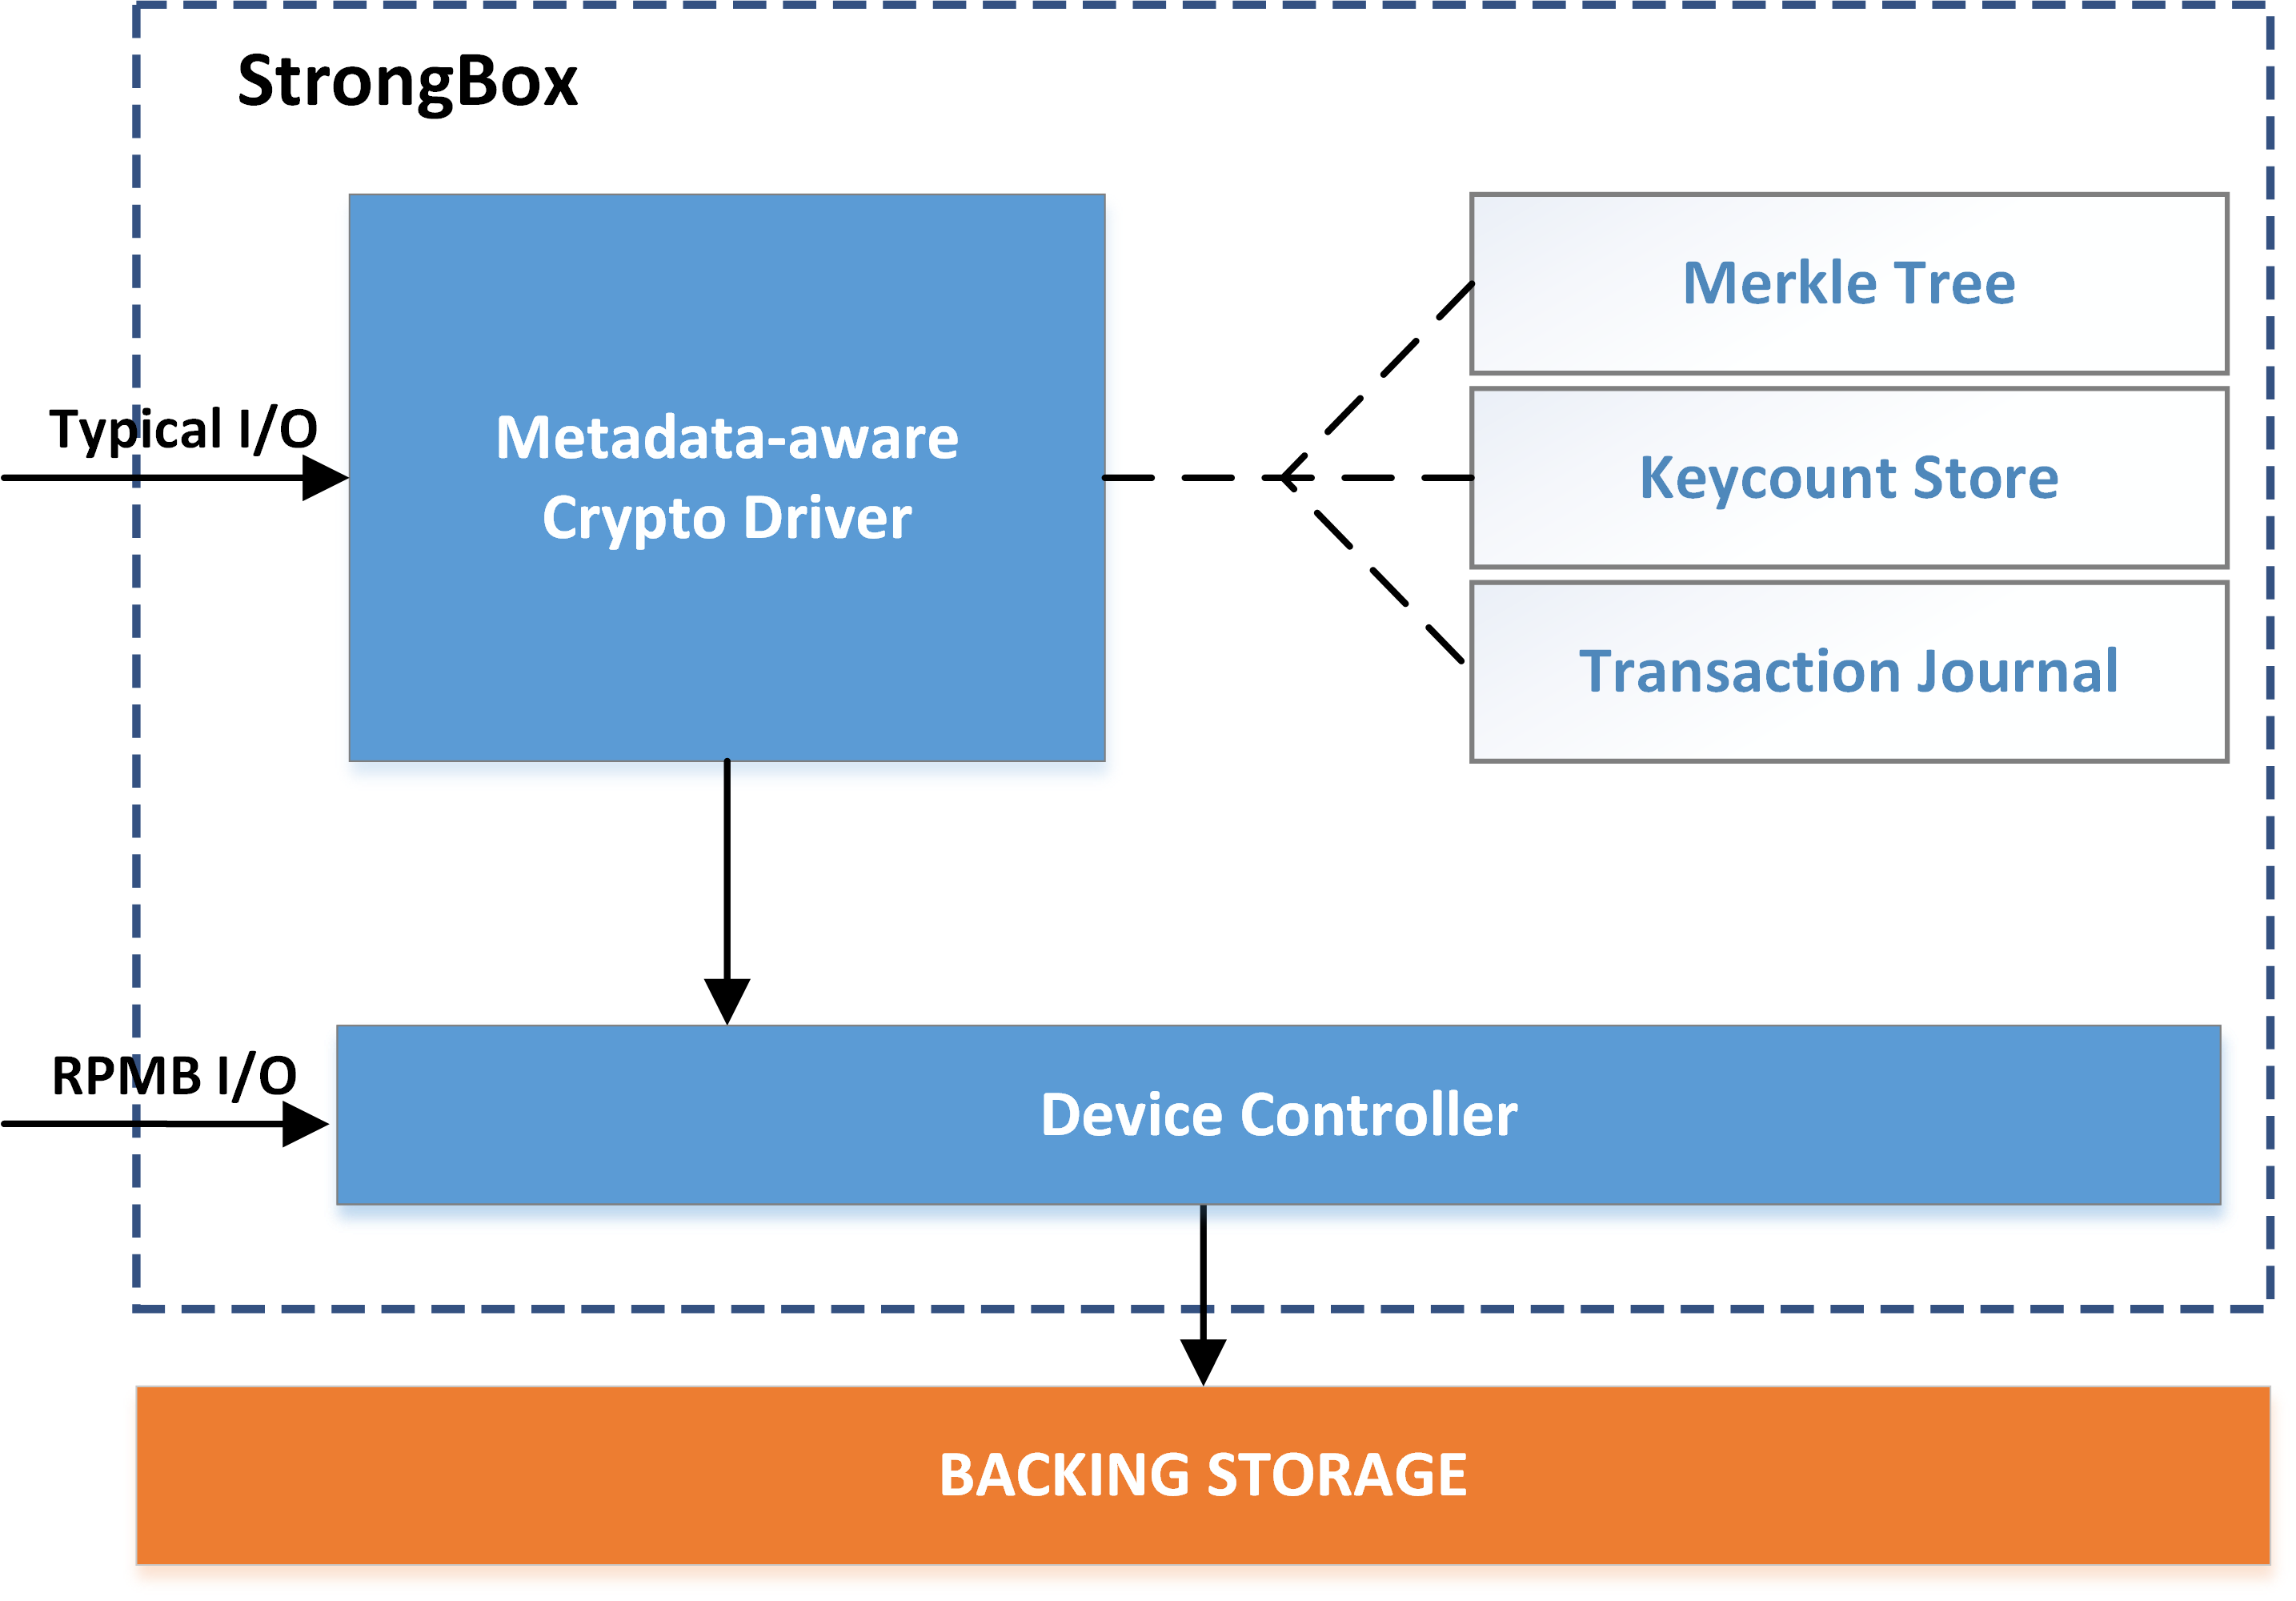
\includegraphics[width=\linewidth]{figs/sc/overview.png}
   \caption{Overview of the SwitchCrypt construction.} \label{fig:overview}
\end{figure}

SwitchCrypt consists of a \emph{Generic Stream Cipher Interface} and
\emph{Cryptographic Driver} and sits between a Log-structured File System (LFS)
on the OS, and the underlying drive (backing storage) and device controller
(e.g. Flash Translation Layer). This is illustrated in \figref{overview}, which
provides an overview of the SwitchCrypt system design.

\begin{figure}[t]
   \centering
   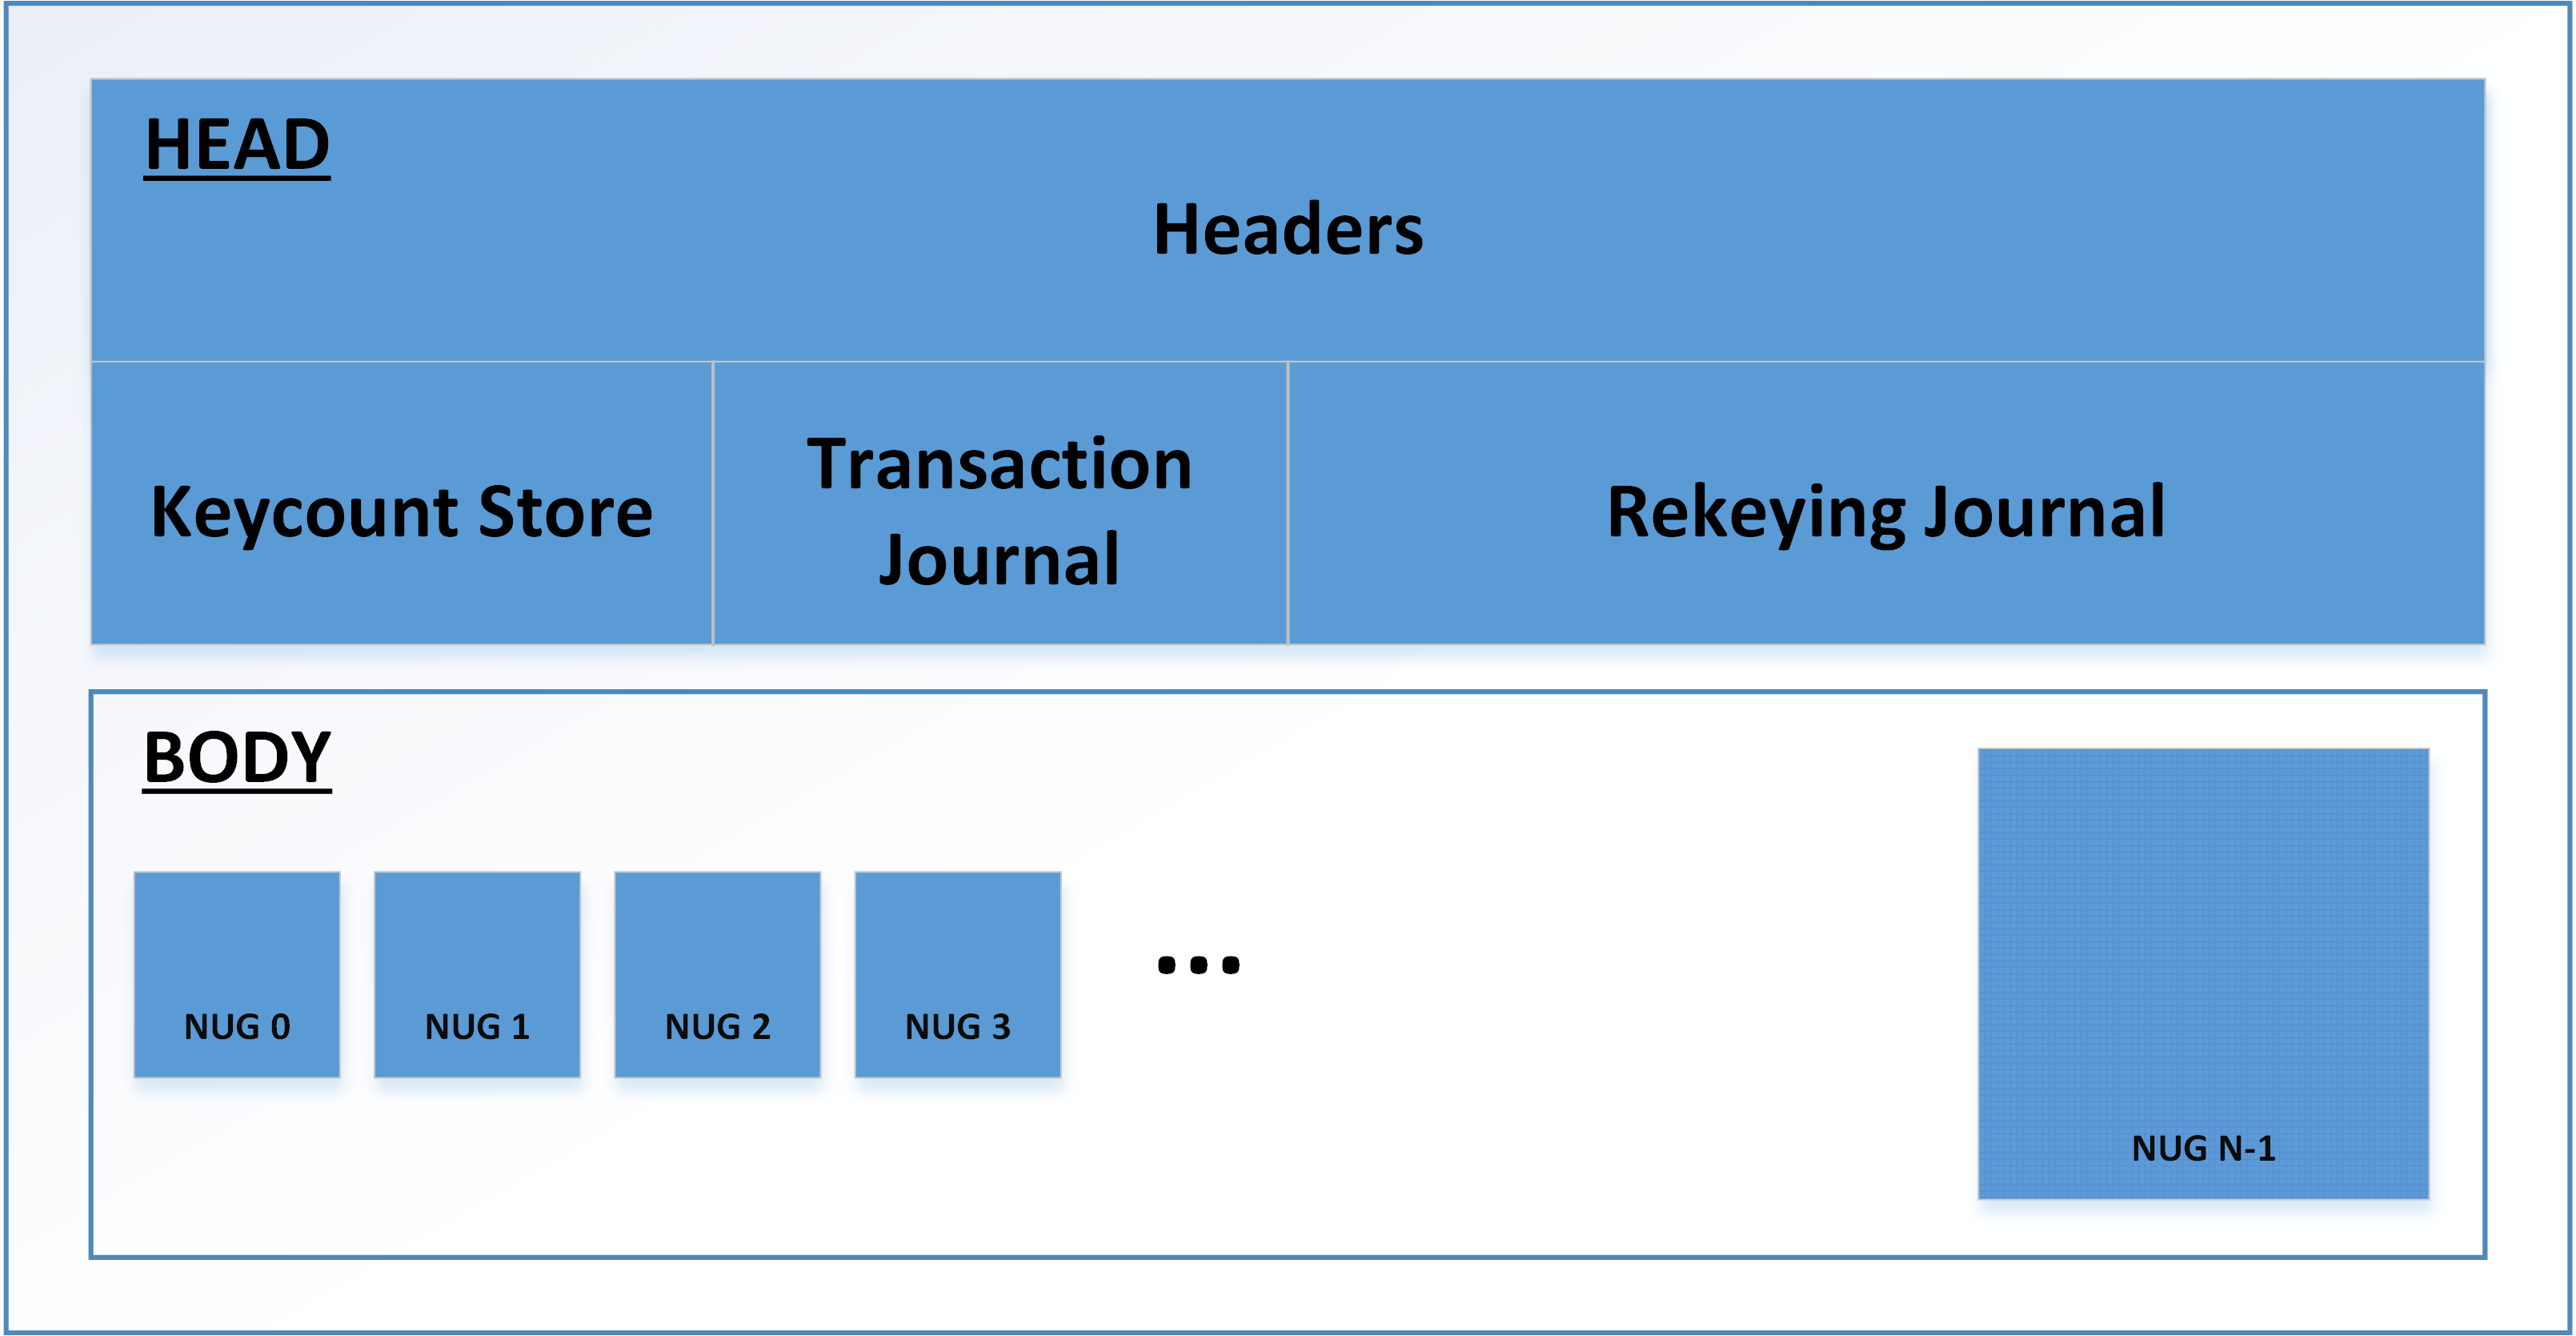
\includegraphics[width=\linewidth]{figs/sc/backstore.png}
   \caption{Layout of SwitchCrypt's drive layout.} \label{fig:backstore}
\end{figure}

The drive itself is divided into a \emph{HEAD} section and \emph{BODY} section
upon initialization, illustrated in \figref{backstore}. The HEAD consists of
metadata headers written during initialization~\cite{StrongBox} along with the
\emph{Keycount Store}, \emph{Transaction Journal}, \emph{Rekeying Journal}, and
\emph{Per-Nugget Metadata}, each drive-backed. These components are used by the
\emph{Cryptographic Driver} together with the \emph{Cipher Switching Strategy}
implementations to enable efficient per-unit cipher switching.

The BODY consists of a series independent same-size logical units called
\emph{nuggets}. A nugget consists of one or more contiguous physical drive
blocks. Each nugget is coupled with metadata in the HEAD indicating which cipher
was used to encrypt the nugget along with any additional ciphertext output; the
latter allows us to treat any non-length-preserving ciphers as if they were
length-preserving. SwitchCrypt uses the Keycount Store and Transaction Journal
components along with our nugget layout to 1) track, detect, and handle
overwrites, 2) limit the maximum length of any plaintext input to ciphers, thus
amortizing the overhead incurred during encryption, and 3) independently and
efficiently switch the cipher used to encrypt individual nuggets.

StrongBox demonstrated how to make nugget-based drive organization secure using
a single stream cipher, ChaCha20, to handle overwrites, prevent rollback
attacks, and limit plaintext length~\cite{StrongBox}. However, StrongBox's was
not designed envisioning the utility in trading off between concerns at the
filesystem or device-mapper level, dynamic cipher switching, or protecting
against attacks on data ``in motion;'' the remainder of this section details the
novel components that enable this functionality. Specifically: how we quantify
the properties traded off between configurations (\cref{subsec:quantify}), the
Generic Stream Cipher Interface and Per-Nugget Metadata components
(\cref{subsec:interface}) which decouple cipher implementations from the
encryption process, and our Cipher Switching Strategy implementations
(\cref{subsec:strategies}) used to efficiently encrypt nuggets with different
ciphers.

\subsection{Quantifying Cipher Security Properties} \label{subsec:quantify}

To reason about when to trade off between the ciphers evaluated in this work, we
must have a way to compare ciphers' utility in the context of SwitchCrypt FDE.
However, different ciphers have a wide range of security properties, performance
profiles, and output characteristics. To address this need, we propose a novel
evaluation framework (see: \tblref{security-quant}). Our framework classifies
stream ciphers according to three quantitative features: relative round count,
ciphertext randomization, and ciphertext expansion. Taken together, these
features reveal a rich tradeoff space of cipher configurations optimizing for
different combinations of concerns.

\begin{table}[ht]
   \centering
   \begin{tabular}{@{}ccccc@{}}
   \toprule
   \textbf{Cipher} & \textbf{Rounds} & \textbf{Randomization} &
   \textbf{Expansion} \\
   \midrule
   ChaCha8         & 0           & 0           & 1           \\
   ChaCha12        & 0.5         & 0           & 1           \\
   ChaCha20        & 1           & 0           & 1           \\
   Salsa8          & 0           & 0           & 1           \\
   Salsa12         & 0.5         & 0           & 1           \\
   Salsa20         & 1           & 0           & 1           \\
   HC128           & 0           & 0           & 1           \\
   HC256           & 1           & 0           & 1           \\
   Freestyle (F)   & 0           & 2           & 0           \\
   Freestyle (B)   & 0.5         & 2.5         & 0           \\
   Freestyle (S)   & 1           & 3           & 0           \\
\end{tabular}
   \caption{Our framework for classifying stream ciphers according to three
   ideal features: relative round count, ciphertext randomization, and
   ciphertext expansion.}
   \label{tbl:security-quant}
 \end{table}

\subsubsection{Relative Rounds (Rounds)}

The ciphers we examine in this work are all constructed around the notion of
\emph{rounds}, where a higher number of rounds (and possibly longer key) is
positively correlated with a higher resistance to brute force given no fatal
related-key or other attacks~\cite{ChaCha-Cryptanalysis}. Hence, this feature
represents how many rounds a cipher executes relative to other implementations
of the same algorithm. For instance: ChaCha8 is a reduced-round version of
ChaCha12, which is a reduced-round version of ChaCha20, all using the ChaCha
algorithm~\cite{ChaCha20,ChaCha-Cryptanalysis}.

We limit our analysis to groups of three implementations, each using a different
number of rounds. In the case of HC-128 and HC-256, we limit our analysis to a
group of two implementations. Scores range from 0 (least number of rounds
considered) to 1 (greatest number of rounds considered).

\subsubsection{Ciphertext Randomization (Randomization)}

A cipher with ciphertext randomization generates different ciphertexts
non-deterministically given the same key, nonce, and plaintext. This makes it
much more difficult to execute chosen-ciphertext attacks (CCA), key
re-installation attacks, XOR-based cryptanalysis and other comparison attacks,
and other confidentiality-violating schemes where the ciphertext is in full
control of the adversary ~\cite{Freestyle}. This property is useful in cases
where we cannot prevent the same key, nonce, and plaintext from being reused,
such as with data ``in motion'' (see the motivational example in
\secref{sc-motivation}). Ciphers without this property---such as ChaCha20 on
which prior work is based---are trivially broken when key-nonce-plaintext
3-tuples are reused. In StrongBox, this is referred to as an ``overwrite
condition'' or simply ``overwrite''~\cite{StrongBox}.

Though there are many ways to achieve ciphertext randomization, the ciphers
included in our analysis implement it using a random number of rounds for each
block of the message where the exact number of rounds are unknown to the
receiver a priori~\cite{Freestyle}. In determining the minimum and maximum
number of rounds used per block in this non-deterministic mode of operation, we
can customize the computational burden an attacker must bear by choosing lower
or higher minimums and maximums. Hence, this is not a binary feature; scores
range from 0 (no ciphertext randomization) to 1 (lowest minimum and maximum
rounds per block) to 3 (highest minimum and maximum rounds per block).

\subsubsection{Ciphertext Expansion (Expansion)}

A cipher that exhibits ciphertext expansion is non-length-preserving: it outputs
more or less ciphertext than was originally input as plaintext. This can cause
major problems in the FDE context. For instance, cryptosystems that rely on
AES-XTS (e.g. Linux's dm-crypt, Microsoft's BitLocker, Apple's FileVault) or
ChaCha (e.g. StrongBox, Google's Adiantum) have storage layouts that hold
length-preserving output as an invariant, making ciphers that do not exhibit
this property incompatible with their implementations; yet, ciphertext expansion
is often (but not always) a necessary side-effect of ciphertext randomization.

The ciphers included in our analysis that exhibit ciphertext expansion have an
overhead of around 1.56\% per plaintext message block~\cite{Freestyle}. Even a
single byte of additional ciphertext vs plaintext would make a cipher
inappropriate for use with prior work. Hence, this is a binary feature in that a
cipher either outputs ciphertext of the same length as its plaintext input or it
does not. A cipher scores either a 0 if it \emph{is not} length-preserving in
this way or a 1 if the ciphertext is always the same length as the plaintext.

\subsection{Generic Stream Cipher Interface} \label{subsec:interface}

One of the goals of SwitchCrypt is that we might use any stream cipher
regardless of its implementation details. Yet this is entirely non-trivial.
There are many cipher implementations that we might use with SwitchCrypt, each
with unique input requirements and output considerations. For instance, Salsa
and Chacha implementations require a certain IV and key size and handle
plaintext input through successive invocations of a single state update
function~\cite{Floodyberry}. Using OpenSSL's AES implementation in CTR mode
requires manually tracking the counter state and individual ciphertext blocks
are retrieved though corresponding function invocations. Freestyle's reference
implementation requires we calculate the extra space necessary per nugget (due
to ciphertext expansion) along with configuration-dependent minimum and maximum
rounds-per-block, hash interval, and pepper bits~\cite{Freestyle}. HC-128 and
other ciphers have similarly disparate requirements.

Unlike prior work, SwitchCrypt must be able to encrypt and decrypt arbitrary
nuggets \emph{with any of these ciphers} at any moment with low overhead and
without tight coupling to any specific implementation detail. Hence, there is a
need for an interface that completely decouples cipher implementations from the
encryption/decryption process. Our novel cipher interface allows any stream
cipher to be integrated into SwitchCrypt without modifications to third-party
code, enabling normally incompatible ciphers to encrypt and decrypt arbitrary
nuggets. The ability for disparate cipher implementations to co-exist forms the
foundation for SwitchCrypt's ability to switch the system between different
cipher configurations in our tradeoff space efficiently and effectively.

To facilitate this, the Generic Stream Cipher Interface presents the
cryptographic driver with a single unified encryption/decryption model.
SwitchCrypt receives I/O requests from the operating system at the block device
level like any other device-mapper. These requests come in the form of either
reads or writes. When a read request is received, the OS hands SwitchCrypt an
offset and a length and expects a response with plaintext of that specific
length starting at that specific offset taken from the beginning of storage
(i.e. the BODY section; see \figref{backstore}). When a write request is
received, the OS hands SwitchCrypt an offset, a length, and a buffer of
plaintext and expects that plaintext to be encrypted and committed to storage
such that the plaintext is later retrievable given that same offset and length
in a future read request. These requests can either be handled together by a
single function or handled individually as distinct read and write operations,
each with different tradeoffs.

\begin{enumerate}
   \item \textbf{\texttt{xor\_interface}}\\\texttt{xor\_interface} executes
   independently of SwitchCrypt internals and treats encryption and decryption
   as the same operation. Implementations receive an integer offset $F$, an
   integer length $L$, a key buffer $K$ corresponding to the current nugget, and
   an empty $L$-length XOR buffer. SwitchCrypt expects the XOR buffer to be
   populated with $L$ bytes of keystream output from some stream cipher seeked
   to offset $F$ with respect to key $K$. The length of the key buffer will
   always be exactly what the cipher implementation expects, alleviating the
   burden of key management; similarly, the XOR buffer will be XOR-ed with the
   appropriate portion of nugget contents automatically, alleviating the burden
   of drive access and other tedious calculations. \\
   \item \textbf{\texttt{read\_interface}} and
   \textbf{\texttt{write\_interface}}\\
   Unlike \texttt{xor\_interface}, encryption and decryption are distinct
   concerns at this abstraction level. \\\texttt{read\_interface} handles
   decryption during reads. \\\texttt{write\_interface} handles encryption
   during writes. Implementations receive full access to SwitchCrypt internals,
   giving wrapper code complete control over the encryption and decryption
   process and allowing implementers to bypass parts of the nugget-based drive
   layout abstraction (i.e. BODY) if necessary. This comes at the cost of 1)
   significantly increased code complexity, as the implementer must perform
   certain I/O manually, distinguish between independent nuggets on the drive,
   determine what to encrypt or decrypt at what offset and when, when to commit
   which metadata and where and 2) potential performance implications, since
   SwitchCrypt must account for not having absolute control over its internal
   data structures during function invocation. For a cipher like Freestyle,
   configurations with lower minimum and maximum rounds per block may see a
   performance improvement here, while configurations with higher minimum and
   maximum rounds per block may see reduced performance.
\end{enumerate}

\subsection{Cipher Switching Strategies} \label{subsec:strategies}

The Generic Stream Cipher Interface allows many differently ciphered nuggets to
co-exist on the same drive. However, at any moment, there is only a single
\emph{active cipher configuration} (henceforth \emph{active configuration}). The
active configuration is used to encrypt nugget contents. When a cipher switch is
triggered, a different configuration becomes the active configuration. At this
point, SwitchCrypt must determine \emph{when} to re-cipher a nugget and
\emph{where} to store the output on the drive. ``Re-ciphering'' here means using
an inactive configuration to decrypt a nugget's contents and using the active
configuration to re-cipher it. Depending on the use case, it may make the most
sense to re-cipher a nugget immediately, or eventually, or to maintain several
areas of differently-ciphered nuggets concurrently.

A naive approach would switch every nugget in BODY to the active configuration
immediately, but the latency and energy cost would be unacceptable. Hence, a
more strategic approach is necessary. We satisfy this need with our \emph{cipher
switching strategies}. These novel strategies allow for nuggets to be
re-ciphered in a variety of cases with minimal impact on performance and battery
life and without compromising security. This is thanks to the nugget-based drive
layout, which limits the churn of cipher switching operations to relatively
small regions of ciphertext on the drive.

Determining \emph{when} to target a nugget for re-ciphering we call
\emph{temporal switching}, for which we propose the \emph{Forward} switching
strategy. Determining \emph{where}---in which storage region and across which
nuggets---to output ciphertext we call \emph{spatial switching}, for which we
propose the \emph{Mirrored} and \emph{Selective} switching strategies. \\

\textbf{Forward Switching Strategy.} When a nugget is encountered during I/O
that was encrypted using something other than the active configuration, the
Forward strategy dictates that this nugget be re-ciphered immediately. If a
particular nugget encrypted with an inactive configuration is never encountered
during I/O, it is never re-ciphered and remains on the drive in its original
state. In this way, the Forward strategy represents a form of temporal cipher
switching.

Rather than re-cipher the entire drive every time the active configuration
changes, this strategy limits the performance impact of cipher switching to
individual nuggets. The expense of re-ciphering is paid only once, after which
the nugget is accessed normally during I/O until the active configuration is
switched again.

There are several forms the Forward strategy might take. The default and
most intuitive is \emph{0-forward}, in which SwitchCrypt immediately transitions
individual nuggets encountered during I/O to the active configuration if they
are not using it. Over time, if various I/O operations end up touching every
nugget in the drive, the encrypted contents of every nugget will become
decryptable with the currently active configuration.

The Forward strategy might also take the form of \emph{N-forward}, where
SwitchCrypt attempts to take advantage of spatial sequential locality to
transition whole sets of nuggets into the active configuration. We can trivially
expand the forward strategy to encompass the entire drive by selecting $N$ equal
to the total number of nuggets managed by SwitchCrypt. This would have the
overhead of re-ciphering large swaths of the drive upon every I/O operation
where a nugget encrypted with the inactive configuration is encountered. Of
course, this has the same dire implications for performance as simply
re-initializing the entire system or encrypted container with the new cipher. \\

\textbf{Selective Switching Strategy.} When SwitchCrypt is initialized with the
Selective strategy, the drive is partitioned into $C$ regions where $C$
represents the total number of available ciphers in the system; each regions'
nuggets are encrypted by each of the $C$ ciphers respectively. For instance,
were SwitchCrypt initialized using two ciphers ($C = 2$), the drive would be
partitioned in half; all nuggets in the first region would be encrypted with the
first cipher while all nuggets in the second would be encrypted with the other.


When using this strategy, the active cipher determines which partition we
``select'' for I/O operations. Hence, unlike the Forward strategy, which
schedules individual nuggets to be re-ciphered at some point in time after the
active configuration is switched, the Selective strategy allows the wider system
to indicate \emph{where} on the drive a read or write operation should occur. In
this way, the Selective strategy represents a form of spatial cipher switching
where different regions of the drive can store differently-ciphered nuggets
independently and concurrently. A user could take advantage of this to, for
instance, set up regions with different security properties and performance
characteristics, managing them as distinct virtual drives or transparently
reading/writing bytes to different security regions on the same drive. \\

\textbf{Mirrored Switching Strategy.} Similar to the Selective strategy, when
SwitchCrypt is initialized with the Mirrored strategy, the drive is partitioned
into $C$ regions where $C$ represents the total number of available ciphers in
the system; each regions' nuggets are encrypted by each of the $C$ ciphers
respectively.

However, unlike the Selective strategy, all write operations that hit one region
are mirrored into the other regions immediately, so all regions of the drive
will always be in a consistent state and always share the same data. The active
configuration determines \emph{where} a read operation should occur. In this
way, the Mirrored strategy represents a form of spatial cipher switching because
we are switching which configuration we are using to read in data. A user could
take advantage of this along with SSD Instant Secure Erase~\cite{ISE1,ISE2,ISE3}
to delete other regions, thus quickly and securely converging the drive to a
single configuration without losing any data or suffering the egregious
performance or battery penalty that comes with re-ciphering every nugget.

\subsubsection{Comparing Cipher Switching Strategies}

\begin{table}[t]
   \centering
   \begin{tabular}{@{}|c|c|c|C{25mm}|@{}}
      \toprule
      \textbf{Strategy} & \textbf{Convergence} & \textbf{Waste} &
      \textbf{Performance} \\
      \midrule
      Forward   & Slower       & None & Faster reads and writes unless switching
      \\\hline
      Mirrored  & Nearly instant & High & Faster reads; slower writes \\
      \hline
      Selective & Slower       & High & Faster reads and writes  \\
      \hline
   \end{tabular}
   \caption{A summary comparison between the three cipher switching strategies.}
   \label{tbl:strategies-advantages}
\end{table}

\tblref{strategies-advantages} summarizes the higher level tradeoffs between the
three cipher switching strategies.

\textbf{Convergence.} Depending on the use case, the ability to quickly converge
the entire drive to a single cipher configuration without losing data is very
useful (see: \secref{sc-usecases}). The near-instantaneous ``just forget the key''
nature of SSD Instant Secure Erase (ISE) implementations on modern
SSDs~\cite{ISE1,ISE2,ISE3} makes this a very fast process for the Mirrored
strategy. The Forward strategy is slow to converge compared to Mirrored since,
in the worse case, every nugget on the drive will require re-ciphering. The
Selective strategy is similarly slow to converge since entire regions of nuggets
must be moved and re-ciphered to prevent data loss; those regions could be
destroyed without moving data around using ISE too, which would be very fast,
but unlike Mirrored some data would be lost forever.

\textbf{Waste.} Unlike the other two strategies, using the Forward strategy does
not reduce the total usable space on the drive by the end-user, ciphertext
expansion notwithstanding. We refer to this as ``waste''. The Forward strategy
is not wasteful in this way because it allows differently-ciphered nuggets to
co-exist contiguously on the drive without special partitions. Since the
Mirrored and Selective strategies require partitioning the drive into some
number of regions---where the writeable size reported back to the OS is some
function of region size---there is a necessary reduction in usable space.

\textbf{Performance.} The Selective and Mirrored strategies can read data from
the drive with low overhead, reaching performance parity with prior work,
because they never have to deal with on-demand re-ciphering. This is because
switching ciphers using these two strategies amounts to offsetting the read
index so that it lands in the proper BODY partition on the drive, which has
little overhead. The Forward strategy also reads with low overhead except in the
case where a nugget was not encrypted with the active configuration. This
triggers re-ciphering on-demand, which can be costly if the workload constantly
touches unique nuggets and is small enough that cost is not amortized.

The Selective strategy also writes with low overhead because, like with reads,
an index offset is the only requirement. The Mirrored strategy, on the other
hand, can be up to two times slower for writes (when $C = 2$) compared to
baseline. Each additional region ($C > 2$) compounds the write penalty depending
on the workload. This is because each write is mirrored across \emph{all}
regions. As with reads, the Forward strategy writes with low overhead except in
the case where a nugget was not encrypted with the active configuration. This
triggers re-ciphering on-demand, which can be costly if the workload touches
unique nuggets and is small enough that cost is not amortized.\\

With these tradeoffs in mind: Mirrored is ideal when the drive must converge
quickly, write performance is not a primary concern, and drive space is
abundant; Selective is ideal when different data should be encrypted differently
and drive space is abundant; and Forward is ideal when some subset of nuggets
should be encrypted differently without wasting drive space. See
\secref{sc-usecases} for specific scenarios that demonstrate these differences in
practice.

\subsubsection{Threat Model for Cipher Switching Strategies}

The primary concern facing any FDE solution is that of confidentiality. An
adversary should not be able to reveal any information about encrypted plaintext
without the proper key. As with prior work, encryption is achieved via a binary
additive approach: cipher output (keystream) is combined with plaintext nugget
contents using XOR, with metadata to track writes and ensure that pad reuse
never occurs during overwrites and that the system can recover from crashes into
a secure state. Another concern is data integrity: an adversary should not be
able to tamper with ciphertext and it go unnoticed. Nugget integrity is tracked
by an in-memory Merkle tree. See the threat model addressed by Dickens et
al.~\cite{StrongBox} for further details.

Switching strategies add an additional security concern not addressed by prior
work: even if we initiate a ``cipher switch,'' there may still be data on the
drive that was encrypted with an inactive configuration. Is this a problem? For
the Forward strategy, this implies data may at any time be encrypted using the
``least desirable cipher''. For the Mirrored and Selective strategies, the drive
is partitioned into regions where nuggets are guaranteed to be encrypted with
each cipher, including the ``least desirable cipher''. However, in terms of
confidentiality, the confidentiality guarantee of SwitchCrypt can be reduced to
the individual confidentiality guarantees of the available ciphers used to
encrypt nuggets.

\subsection{Putting It All Together} \label{subsec:summary}

We revisit the motivating example from \secref{sc-motivation}, where we are
using Freestyle to ensure secure backups. Initially, I/O requests come down from
the LFS and are received by the cryptographic driver, which divides the request
based on which nuggets it touches. For each nugget, the per-nugget metadata is
consulted to determine with which cipher the nugget is encrypted. If it is
encrypted with the active cipher configuration (Freestyle), which must be true
if we have not initiated a cipher switch, the write is handled similarly to
prior work: encrypted data is read in from the drive, the merkle tree and
monotonic counter are consulted to ensure the integrity of encrypted data, the
transaction journal is consulted during write operations so that overwrites are
handled and pad reuse violations are avoided, and then the keycount store is
consulted to derive the nugget's unique encryption key from some master secret.
Finally, using the Generic Stream Cipher Interface, we call out to the
Freestyle, allowing SwitchCrypt to encrypts/decrypts the nugget's contents and
commit any updates back to storage. All the while, the drive's
Freestyle-encrypted contents are being uploaded up to our enterprise backup
service every so often.

When the device enters ``battery saver'' mode, drive backups are paused, the
energy monitoring software downclocks the CPU, and the OS signals to SwitchCrypt
that a more energy-efficient cipher (ChaCha20) should be used until we return to
a non-curtailed energy budget. SwitchCrypt sets ChaCha20 as the active cipher
configuration. Now, when the cryptographic driver divides I/O requests into each
affected nugget, the per-nugget metadata shows SwitchCrypt that each nugget is
encrypted using a cipher that is not the active configuration. This triggers the
re-ciphering code path. Since we are using the Forward switching strategy in
this example, nugget data is immediately decrypted by calling out to the
inactive configuration through the Generic Stream Cipher Interface, after which
the nugget is re-ciphered by calling out to the active configuration. Finally,
the cryptographic driver manages encrypting/decrypting data and updating the
merkle tree and monotonic counter, transaction journal, and keycount store as
the I/O operation and related metadata is committed to the drive afterwards.

Now, thanks to SwitchCrypt, the system can adapt to changing requirements beyond
the capability of prior work. See \secref{sc-usecases} for specifics.

\section{Implementation} \label{sec:sc-implementation}

Our SwitchCrypt implementation consists of 9,491 lines of C code; our test suite
consists of 6,077 lines of C code. All together, our solution is comprised of
15,568 lines of C code. Our implementation is also publicly available
open-source\footnoteref{note1}.

SwitchCrypt uses OpenSSL version 1.1.0h and LibSodium version 1.0.12 for its
AES-XTS and AES-CTR implementations. Open source ARM NEON optimized
implementations of ChaCha are provided by Floodyberry~\cite{Floodyberry}. The
Freestyle cipher reference implementation is from the original Freestyle
paper~\cite{Freestyle}. The eSTREAM Profile 1 cipher implementations are from
the open source libestream cryptographic library~\cite{libestream} by Lucas
Clemente Vella. The Merkle Tree implementation is from the Secure Block
Device~\cite{SBD}.

We implement SwitchCrypt on top of the BUSE~\cite{BUSE} virtual block device,
using it as our mock device controller. BUSE is a thin (200 LoC) wrapper around
the standard Linux Network Block Device (NBD). BUSE allows an operating system
to transact block I/O requests to and from virtual block devices exposed via
domain socket.

For experimental purposes, our implementation makes the choice of ciphers
binary: either the system wants SwitchCrypt to access the backing store using
the active cipher or the inactive cipher. However, there is no technical
limitation preventing various different nuggets encrypted with three, four, or
more unique ciphers.

We use POSIX message queues to indicate intent to switch. A production-ready
implementation would be greatly simplified by adding an ``intent'' parameter to
the POSIX \textit{read()} and \textit{write()} system calls, allowing
SwitchCrypt to more exactly map individual I/O operations to specific areas of
the backing store when spatially switching. We simulate this with IPC. This is
especially important when considering the selective switching strategy; a
production-ready implementation supporting selective switching would need to
differentiate between metadata operations belonging to the filesystem (should be
mirrored across all regions) and actual end-user data (should be selectively
read from and written to nuggets in specific regions).

Further, to operate securely, SwitchCrypt must be seeded with random data
initially rather than have the backing store consist of all zeroes. This is a
one-time cost paid during initialization and has no tangible effect on
performance. SSDs that support ISE can accomplish this with minimal wear.

Finally, as the Freestyle cipher is highly configurable, we implement it in
three different configurations: a ``fast'' mode with parameters
\\\texttt{FreestyleFast($R_{min}$=$8$, $R_{max}$=$20$, $H_I$=$4$, $I_C$=$8$)}, a
``balanced'' mode with parameters \texttt{FreestyleBalanced($R_{min}$=$12$,
$R_{max}$=$28$, $H_I$=$2$, $I_C$=$10$)}, and a ``strong'' mode with parameters
\texttt{FreestyleStrong($R_{min}$=$20$, $R_{max}$=$36$, $H_I$=$1$, $I_C$=$12$)}.

Thanks to Freestyle's output randomization (see \secref{sc-design}), we can skip
the overhead of tracking, detecting, and handling overwrites when nuggets are
using it, offsetting the 1.6x to 3.2x performance loss of using Freestyle versus
ChaCha20~\cite{Freestyle}.

\subsection{Implementing Cipher Switching}

A naive implementation is trivial (\eg{execute the chosen strategy on every I/O
operation}), this navigation must occur with acceptable overhead by preserving
performance wherever possible. Our cryptographic driver provides such a
mechanism, tying together cipher switching strategies.

In the cases of Mirrored and Selective switching, we use offset to determine in
which area of the backing store receives I/O.

In the case of Forward switching, it is tempting to implement it such that a
nugget is completely re-ciphered during I/O every time its metadata indicates
that it was previously encrypted using a non-active cipher. However, such a
naive implementation can have disastrous effects on performance.

First, a nugget is considered \emph{pristine} if it has not had any data written
into it yet. SwitchCrypt determines if a nugget is pristine by checking the
state of the transaction journal for that nugget. All nuggets start out pristine
with metadata indicating that they are to be encrypted and decrypted by the
initially active cipher. This is true \emph{even if the nugget has not been
written to yet}. This means, on read and write operations after a different
cipher becomes the active cipher configuration using a naively implemented
forward switching strategy, every write operation will trigger a re-keying,
which carries significant overhead.

Our solution was to divide forward switching into \emph{soft re-ciphering} and
\emph{hard re-ciphering}. During soft re-ciphering, only the nugget's metadata
is changed to indicate that the nugget can be encrypted and decrypted with the
newly active cipher configuration but \emph{without actually re-ciphering the
nugget data itself}. This keeps the nugget in its pristine condition, preserving
SwitchCrypt's ability to write data into it without triggering a costly
re-keying operation every time. On the other hand, during hard re-cipher, the
nugget's metadata is changed to match the active cipher configuration \emph{and}
the nugget data is encrypted using the new cipher.

When using forward switching other that 0-forward, \ie{N-forward} where $N > 0$,
only read operations are allowed to trigger hard re-ciphering for nuggets other
than the currently active nugget. This is still not enough to preserve our
performance advantage, however, as I/O operations can span multiple nuggets, and
attempting to take advantage of spatial locality after interacting with every
nugget is counterproductive. Hence, only the last nugget touched by a read
operation will trigger the more aggressive N-forward behavior if $N > 0$. These
considerations have the effect of 1) preserving our performance advantage and 2)
allowing more aggressive N-forward behavior (where $N > 0$) to take advantage of
spatial locality during read-heavy workloads to result in a further performance
advantage (see: \secref{sc-evaluation}).

\section{Evaluation} \label{sec:sc-evaluation}

We implement SwitchCrypt and our experiments on a Hardkernel Odroid XU3 ARM
big.LITTLE system with Samsung Exynos 5422 A15/A7 heterogeneous multi-processing
quad core CPUs at maximum clock speed, 2 gigabyte LPDDR3 RAM at 933 MHz, and an
eMMC5.0 HS400 backing store running Ubuntu Trusty 14.04.6 LTS, kernel version
3.10.106. Energy monitoring was provided by the Odroid's integrated INA-231
power sensors polled every $\approx{260}$ milliseconds (not including
noise/overhead).

We evaluate SwitchCrypt using a Linux RAM disk (tmpfs). The maximum theoretical
memory bandwidth for this Odroid model is 14.9GB/s\@. Our observed maximum
memory bandwidth is 4.5GB/s. Using a RAM disk focuses the evaluation on the
performance differences due to different ciphers.

In each experiment below, we evaluate SwitchCrypt on two high level workloads:
sequential and random I/O. In both workloads, a number of bytes are written and
then read (either 4KB, 512KB, 5MB, 40MB) 10 times. Each workload is repeated
three times for a total of 240 tests per cipher (720 runs per cipher
pair/ratios, explained below); 30 results per byte size, 120 results per
workload. Results are accumulated and the median is taken for each byte size.

When evaluating switching strategies, a finer breakdown in workloads is made
using a pre-selected pair of ciphers we call the \emph{primary cipher
configuration} and \emph{secondary cipher configuration}. SwitchCrypt is
initialized at the primary configuration. Once we trigger a cipher switch,
SwitchCrypt moves towards the secondary configuration via switching strategy.

The cipher switch is triggered according to a certain \emph{ratio} of I/O
operations. For example: given 10 40MB read-write operations, we may write and
then read back 40MB 3 times using the primary cipher, initiate a cipher switch,
and then write and then read back (write-read) 40MB 7 times. This would be a 3:7
ratio. It follows that there are three ratios we use to evaluate SwitchCrypt's
performance in this regard: 7:3, 5:5, and 3:7. Respectively, that is 7 file
write-read operation in the primary cipher for every 3 file write-read
operations in the secondary cipher (7:3), 7 file write-read operation in the
primary cipher for every other file write-read operation in the secondary cipher
(5:5), and 3 file write-read operations in the primary cipher for every 7 file
write-read operation in the secondary cipher (3:7).

All experiments are performed with basic Linux I/O commands, bypassing system
caching.

In this section we answer the following questions:

\begin{enumerate}
 \item What shape does the cipher configuration tradeoff space take under our
 workloads? (\cref{subsec:1})
 \item Can SwitchCrypt achieve dynamic security/energy tradeoffs by reaching
 configuration points not accessible with prior work? (\cref{subsec:2})
 \item What is the performance and storage overhead of each cipher switching
 strategy? (\cref{subsec:3})
\end{enumerate}

\subsection{Switching Strategies Under Various Workloads} \label{subsec:1}

\begin{figure}[ht]
  \textbf{Baseline Cipher I/O Performance}\par\medskip
  {\begin{tikzpicture}[baseline]

    \pgfmathsetmacro{\ymax}{1.1} % set the maximum y value
    \pgfmathsetmacro{\ymaxbreak}{1.2} % set the y value at which overflow is drawn

    \begin{groupplot}[
        group style={
            group size=2 by 2,
            xlabels at=edge bottom,
            ylabels at=edge left,
            xticklabels at=edge bottom,
            yticklabels at=edge left,
            vertical sep=25pt,
            horizontal sep=15pt,
        },
        %axis x line*=bottom,
        height=3.5cm,
        width=\linewidth/1.75,
        tick align=outside,
        tick pos=bottom, % make sure ticks only appear at the bottom and left axes
        title style={yshift=-1.5ex},
        tick style={ black },
        y tick label style={ /pgf/number format/fixed, /pgf/number format/precision=0 },
        grid style={ dotted, gray },
        scatter,
        point meta=explicit symbolic,
        scatter/classes={
            c8={mark=square*},
            c20={mark=triangle*},
            ff={mark=diamond*},
            fb={mark=pentagon*},
            fs={mark=otimes}
        },
        %every node near coord/.append style={font=\tiny},
        %
        % magic to make the numbers appear above the overly long bars:
        % visualization depends on={rawy \as \rawy}, % save original y values
        % restrict y to domain*={ % now clip/restrict any y value to ymax
        %     \pgfkeysvalueof{/pgfplots/ymin}:\ymaxbreak
        % },
        % after end axis/.code={ % draw squiggly line indicating break
        %     \draw [semithick, white, decoration={snake,amplitude=0.1mm,segment length=0.75mm,post length=0.375mm}, decorate] (rel axis cs:0,1.01) -- (rel axis cs:1,1.01);
        % },
        % nodes near coords={\color{.!75!black}\pgfmathprintnumber\rawy}, % print the original y values (darkened in case they are too light)...
        % nodes near coords greater equal only=\ymax, % ... but ONLY if they are >= ymax
        % clip=false, % allow clip to protrude beyond ymax
        % Custom stuff to edit per template
        %
        xlabel={\footnotesize Security Score},
        xlabel near ticks,
        %xlabel shift={-1.5mm},
        xmin=0, xmax=4,
        xtick={ 0, 1, 2, 3, 4 },
        xticklabels={ 0,,, 3, \empty },
        %major x tick style=transparent,
        %enlarge x limits=0.2, % add some breathing room along the x axis's sides
        %
        ylabel={\footnotesize Latency (normalized)},
        ylabel near ticks,
        ylabel shift={-1.5mm},
        ymajorgrids=true,
        ymin=0, ymax=\ymax,
        ytick={ 0, 1, \ymax },
        yticklabels={ 0, 1, \empty },
        %yticklabels={ 0, 0.5, 1.5, 2 },
        % extra y ticks={1},
        % extra y tick style={grid=major, grid style={dashed, black}},
        % extra y tick label={\empty},
        %bar width=4.5pt, % change size of bars
        %
        legend cell align=center,
        legend style={ column sep=1ex },
        legend entries={%
            {\scriptsize 4K},
            {\scriptsize 512K},
            {\scriptsize 5M},
            {\scriptsize 40M}
        },
        legend style={
            draw=none,
            legend columns=4,
            at={(1.0,1.35)},
            anchor=south,
        },
    ]
        \nextgroupplot[title={Sequential Reads}]
            \addlegendimage{no markers,red}
            \addlegendimage{no markers,green,dashed}
            \addlegendimage{no markers,blue,dashdotted}
            \addlegendimage{no markers,orange,densely dotted}
            \addplot [thick, red] table [
                meta=cipher,
                x=score,
                y=latency,
                discard if symbol not={iop}{4k-r},
                discard if symbol not={order}{seq},
                col sep=space,
            ] {data/sc/tradeoff-baseline.dat};
            % \label[c8]{fig:tnr:c8}
            % \label[c20]{fig:tnr:c20}
            % \label[ff]{fig:tnr:ff}
            % \label[fb]{fig:tnr:fb}
            % \label[fs]{fig:tnr:fs}
            \addplot [thick, dashed, green] table [
                meta=cipher,
                x=score,
                y=latency,
                discard if symbol not={iop}{512k-r},
                discard if symbol not={order}{seq},
                col sep=space
            ] {data/sc/tradeoff-baseline.dat};
            \addplot [thick, dashdotted, blue] table [
                meta=cipher,
                x=score,
                y=latency,
                discard if symbol not={iop}{5m-r},
                discard if symbol not={order}{seq},
                col sep=space
            ] {data/sc/tradeoff-baseline.dat};
            \addplot [thick, densely dotted, orange] table [
                meta=cipher,
                x=score,
                y=latency,
                discard if symbol not={iop}{40m-r},
                discard if symbol not={order}{seq},
                col sep=space
            ] {data/sc/tradeoff-baseline.dat};
        \nextgroupplot[legend to name={throwaway1}, title={Random Reads}]
            \addplot [thick, red] table [
                meta=cipher,
                x=score,
                y=latency,
                discard if symbol not={iop}{4k-r},
                discard if symbol not={order}{rnd},
                col sep=space,
            ] {data/sc/tradeoff-baseline.dat};
            \addplot [thick, dashed, green] table [
                meta=cipher,
                x=score,
                y=latency,
                discard if symbol not={iop}{512k-r},
                discard if symbol not={order}{rnd},
                col sep=space
            ] {data/sc/tradeoff-baseline.dat};
            \addplot [thick, dashdotted, blue] table [
                meta=cipher,
                x=score,
                y=latency,
                discard if symbol not={iop}{5m-r},
                discard if symbol not={order}{rnd},
                col sep=space
            ] {data/sc/tradeoff-baseline.dat};
            \addplot [thick, densely dotted, orange] table [
                meta=cipher,
                x=score,
                y=latency,
                discard if symbol not={iop}{40m-r},
                discard if symbol not={order}{rnd},
                col sep=space
            ] {data/sc/tradeoff-baseline.dat};
        \nextgroupplot[legend to name={throwaway2}, title={Sequential Writes}]
            \addplot [thick, red] table [
                meta=cipher,
                x=score,
                y=latency,
                discard if symbol not={iop}{4k-w},
                discard if symbol not={order}{seq},
                col sep=space,
            ] {data/sc/tradeoff-baseline.dat};
            \addplot [thick, dashed, green] table [
                meta=cipher,
                x=score,
                y=latency,
                discard if symbol not={iop}{512k-w},
                discard if symbol not={order}{seq},
                col sep=space
            ] {data/sc/tradeoff-baseline.dat};
            \addplot [thick, dashdotted, blue] table [
                meta=cipher,
                x=score,
                y=latency,
                discard if symbol not={iop}{5m-w},
                discard if symbol not={order}{seq},
                col sep=space
            ] {data/sc/tradeoff-baseline.dat};
            \addplot [thick, densely dotted, orange] table [
                meta=cipher,
                x=score,
                y=latency,
                discard if symbol not={iop}{40m-w},
                discard if symbol not={order}{seq},
                col sep=space
            ] {data/sc/tradeoff-baseline.dat};
        \nextgroupplot[legend to name={throwaway3}, title={Random Writes}]
            \addplot [thick, red] table [
                meta=cipher,
                x=score,
                y=latency,
                discard if symbol not={iop}{4k-w},
                discard if symbol not={order}{rnd},
                col sep=space,
            ] {data/sc/tradeoff-baseline.dat};
            \addplot [thick, dashed, green] table [
                meta=cipher,
                x=score,
                y=latency,
                discard if symbol not={iop}{512k-w},
                discard if symbol not={order}{rnd},
                col sep=space
            ] {data/sc/tradeoff-baseline.dat};
            \addplot [thick, dashdotted, blue] table [
                meta=cipher,
                x=score,
                y=latency,
                discard if symbol not={iop}{5m-w},
                discard if symbol not={order}{rnd},
                col sep=space
            ] {data/sc/tradeoff-baseline.dat};
            \addplot [thick, densely dotted, orange] table [
                meta=cipher,
                x=score,
                y=latency,
                discard if symbol not={iop}{40m-w},
                discard if symbol not={order}{rnd},
                col sep=space
            ] {data/sc/tradeoff-baseline.dat};
    \end{groupplot}%
\end{tikzpicture}%
} \caption{Median sequential and random
  write and then read performance baseline.}
 \label{fig:tradeoff-no-ratios}
\end{figure}

\figref{tradeoff-no-ratios} shows the relative round count, ciphertext
randomization, and ciphertext expansion scores versus median normalized latency
tradeoff between different stream cipher configurations for our sequential and
random I/O workloads. Trends for median hold when looking at tail latencies as
well. Each line represents one workload: 4KB, 512KB, 5MB, and 40MB respectively
(see legend). Each symbol represents one of our ciphers: ChaCha8, ChaCha20,
Freestyle Fast, Freestyle Balanced, and Freestyle Strong. Of the ciphers we
tested, those with higher round counts and higher ciphertext randomization
scores resulted in higher latency and increased energy use for I/O operations.
The relationship between these concerns is not simply linear, however, which
exposes a rich tradeoff space.

Besides the 4KB workload, the shape of each workload follows a similar trend,
hence we will focus on 40MB and 4KB workloads going forward. Due to the overhead
of metadata management and the fast completion time of the 4KB workloads
(\ie{little time for amortization of overhead}), ChaCha8 and ChaCha20 take
longer to complete than Freestyle Fast. This advantage is not enough to make
Freestyle Balanced or Secure workloads complete faster than the ChaCha variants,
however.

Though ChaCha8 is faster than ChaCha20, there is some variability in
our timing setup when capturing extremely fast events occurring close together
in time. This is why ChaCha8 sometimes appears with higher latency than ChaCha20
for normalized 4KB workloads. ChaCha8 is not slower than ChaCha20.

\subsection{Reaching Between Static Configuration Points} \label{subsec:2}

\begin{figure}[ht]
  \textbf{Forward Switching I/O Ratio Performance}\par\medskip
  {\begin{tikzpicture}[baseline]

    \pgfmathsetmacro{\ymax}{1.1} % set the maximum y value
    \pgfmathsetmacro{\ymaxbreak}{1.2} % set the y value at which overflow is drawn

    \begin{groupplot}[
        group style={
            group size=2 by 2,
            xlabels at=edge bottom,
            ylabels at=edge left,
            xticklabels at=edge bottom,
            yticklabels at=edge left,
            vertical sep=25pt,
            horizontal sep=15pt,
        },
        %axis x line*=bottom,
        height=3.5cm,
        width=\linewidth/1.75,
        tick align=outside,
        tick pos=bottom, % make sure ticks only appear at the bottom and left axes
        title style={yshift=-1.5ex},
        tick style={ black },
        y tick label style={ /pgf/number format/fixed, /pgf/number format/precision=0 },
        grid style={ dotted, gray },
        scatter,
        point meta=explicit symbolic,
        scatter/classes={
            c8={mark=square*},
            c20={mark=triangle*},
            ff={mark=diamond*},
            fb={mark=pentagon*},
            fs={mark=otimes}
        },
        %every node near coord/.append style={font=\tiny},
        %
        % magic to make the numbers appear above the overly long bars:
        % visualization depends on={rawy \as \rawy}, % save original y values
        % restrict y to domain*={ % now clip/restrict any y value to ymax
        %     \pgfkeysvalueof{/pgfplots/ymin}:\ymaxbreak
        % },
        % after end axis/.code={ % draw squiggly line indicating break
        %     \draw [semithick, white, decoration={snake,amplitude=0.1mm,segment length=0.75mm,post length=0.375mm}, decorate] (rel axis cs:0,1.01) -- (rel axis cs:1,1.01);
        % },
        % nodes near coords={\color{.!75!black}\pgfmathprintnumber\rawy}, % print the original y values (darkened in case they are too light)...
        % nodes near coords greater equal only=\ymax, % ... but ONLY if they are >= ymax
        % clip=false, % allow clip to protrude beyond ymax
        % Custom stuff to edit per template
        %
        xlabel={\footnotesize R+R (norm)},
        xlabel near ticks,
        %xlabel shift={-1.5mm},
        xmin=0, xmax=4,
        xtick={ 0, 0.5, 1, 2, 3, 4 },
        xticklabels={ ,0,,, 1, \empty },
        %major x tick style=transparent,
        %enlarge x limits=0.2, % add some breathing room along the x axis's sides
        %
        ylabel={\footnotesize Latency},
        ylabel near ticks,
        ylabel shift={-1.5mm},
        ymajorgrids=true,
        ymin=0, ymax=\ymax,
        ytick={ 0, 1, \ymax },
        yticklabels={ 0, 1, \empty },
        %yticklabels={ 0, 0.5, 1.5, 2 },
        % extra y ticks={1},
        % extra y tick style={grid=major, grid style={dashed, black}},
        % extra y tick label={\empty},
        %bar width=4.5pt, % change size of bars
        %
        legend cell align=left,
        legend style={ column sep=1ex },
        legend entries={
            {\scriptsize Baseline},
            {\scriptsize Ratios},
            {\scriptsize },
            {\scriptsize },
            {\scriptsize },
            {\scriptsize C8},
            {\scriptsize C20},
            {\scriptsize FF},
            {\scriptsize FB},
            {\scriptsize FS}
        },
        legend style={
            draw=none,
            legend columns=5,
            at={(1.0,1.35)},
            anchor=south,
        },
    ]
        \nextgroupplot[title={Sequential 40M Reads}]
            \addlegendimage{no markers,red}
            \addlegendimage{mark=otimes*,only marks,black}
            \addlegendimage{only marks,mark=square*,white}
            \addlegendimage{only marks,mark=square*,white}
            \addlegendimage{only marks,mark=square*,white}
            \addlegendimage{only marks,mark=square*,red}
            \addlegendimage{only marks,mark=triangle*,red}
            \addlegendimage{only marks,mark=diamond*,red}
            \addlegendimage{only marks,mark=pentagon*,red}
            \addlegendimage{only marks,mark=otimes,red}
            \addplot [thick, red] table [
                meta=cipher,
                x=score,
                y=latency,
                discard if symbol not={iop}{40m-r},
                discard if number not={ratio}{0},
                discard if symbol not={order}{seq},
                col sep=space,
            ] {data/sc/tradeoff-ratios.dat};
            \addplot [only marks] table [
                x=score,
                y=latency,
                discard if symbol not={iop}{40m-r},
                discard if number not={ratio}{1},
                discard if symbol not={order}{seq},
                col sep=space
            ] {data/sc/tradeoff-ratios.dat};
            \addplot [only marks] table [
                x=score,
                y=latency,
                discard if symbol not={iop}{40m-r},
                discard if number not={ratio}{2},
                discard if symbol not={order}{seq},
                col sep=space
            ] {data/sc/tradeoff-ratios.dat};
            \addplot [only marks] table [
                x=score,
                y=latency,
                discard if symbol not={iop}{40m-r},
                discard if number not={ratio}{3},
                discard if symbol not={order}{seq},
                col sep=space
            ] {data/sc/tradeoff-ratios.dat};
        \nextgroupplot[legend to name={throwaway4}, title={Sequential 4K Reads}]
            \addplot [thick, red] table [
                meta=cipher,
                x=score,
                y=latency,
                discard if symbol not={iop}{4k-r},
                discard if number not={ratio}{0},
                discard if symbol not={order}{seq},
                col sep=space,
            ] {data/sc/tradeoff-ratios.dat};
            \addplot [only marks] table [
                x=score,
                y=latency,
                discard if symbol not={iop}{4k-r},
                discard if number not={ratio}{1},
                discard if symbol not={order}{seq},
                col sep=space
            ] {data/sc/tradeoff-ratios.dat};
            \addplot [only marks] table [
                x=score,
                y=latency,
                discard if symbol not={iop}{4k-r},
                discard if number not={ratio}{2},
                discard if symbol not={order}{seq},
                col sep=space
            ] {data/sc/tradeoff-ratios.dat};
            \addplot [only marks] table [
                x=score,
                y=latency,
                discard if symbol not={iop}{4k-r},
                discard if number not={ratio}{3},
                discard if symbol not={order}{seq},
                col sep=space
            ] {data/sc/tradeoff-ratios.dat};
        \nextgroupplot[legend to name={throwaway5}, title={Sequential 40M Writes}]
            \addplot [thick, red] table [
                meta=cipher,
                x=score,
                y=latency,
                discard if symbol not={iop}{40m-w},
                discard if number not={ratio}{0},
                discard if symbol not={order}{seq},
                col sep=space,
            ] {data/sc/tradeoff-ratios.dat};
            \addplot [only marks] table [
                x=score,
                y=latency,
                discard if symbol not={iop}{40m-w},
                discard if number not={ratio}{1},
                discard if symbol not={order}{seq},
                col sep=space
            ] {data/sc/tradeoff-ratios.dat};
            \addplot [only marks] table [
                x=score,
                y=latency,
                discard if symbol not={iop}{40m-w},
                discard if number not={ratio}{2},
                discard if symbol not={order}{seq},
                col sep=space
            ] {data/sc/tradeoff-ratios.dat};
            \addplot [only marks] table [
                x=score,
                y=latency,
                discard if symbol not={iop}{40m-w},
                discard if number not={ratio}{3},
                discard if symbol not={order}{seq},
                col sep=space
            ] {data/sc/tradeoff-ratios.dat};
        \nextgroupplot[legend to name={throwaway6}, title={Sequential 4K Writes}]
            \addplot [thick, red] table [
                meta=cipher,
                x=score,
                y=latency,
                discard if symbol not={iop}{4k-w},
                discard if number not={ratio}{0},
                discard if symbol not={order}{seq},
                col sep=space,
            ] {data/sc/tradeoff-ratios.dat};
            \addplot [only marks] table [
                x=score,
                y=latency,
                discard if symbol not={iop}{4k-w},
                discard if number not={ratio}{1},
                discard if symbol not={order}{seq},
                col sep=space
            ] {data/sc/tradeoff-ratios.dat};
            \addplot [only marks] table [
                x=score,
                y=latency,
                discard if symbol not={iop}{4k-w},
                discard if number not={ratio}{2},
                discard if symbol not={order}{seq},
                col sep=space
            ] {data/sc/tradeoff-ratios.dat};
            \addplot [only marks] table [
                x=score,
                y=latency,
                discard if symbol not={iop}{4k-w},
                discard if number not={ratio}{3},
                discard if symbol not={order}{seq},
                col sep=space
            ] {data/sc/tradeoff-ratios.dat};
    \end{groupplot}
\end{tikzpicture}%
} \caption{Median sequential and random
  write and then read back performance comparison of Forward switching to
  baseline. Each cluster of 3 dots between configurations represents the 7:3,
  5:5, and 3:7 primary-vs-secondary I/O ratios described in the text.}
 \label{fig:tradeoff-with-ratios}
\end{figure}

\figref{tradeoff-with-ratios} shows the relative round count, ciphertext
randomization, and ciphertext expansion scores versus median normalized latency
tradeoff between different stream ciphers for our sequential and random I/O
workloads with cipher switching using the Forward strategy. After a certain
number of write-read I/O operations, a cipher switch is initiated and
SwitchCrypt begins using the secondary cipher to encrypt and decrypt data. For
each pair of ciphers, this is repeated three times: once at every ratio point
\emph{between} our static configuration points (\ie{7:3, 5:5, and 3:7 described
above}).

The point of this experiment is to determine if SwitchCrypt can effectively
transition the drive between ciphers without devastating performance. For the
40MB, 5MB, and 512KB workloads (40MB is shown), we see that SwitchCrypt can
achieve dynamic security/energy tradeoffs reaching points not accessible with
prior work, all with minimal overhead.

Again, due to the overhead of metadata management for non-Freestyle ciphers (see
\secref{sc-implementation}) and the fast completion time of the 4KB workloads
preventing SwitchCrypt from taking advantage of amortization, ChaCha8 and
ChaCha20 take longer to complete than Freestyle Fast for 4KB reads. We also see
very high latency for ratios between Freestyle Fast and Freestyle Strong cipher
configurations. This is because Freestyle is not length-preserving, so extra
write operations must be performed, and the algorithm itself is generally much
slower than the ChaCha variants (see \figref{tradeoff-no-ratios}). Doubly
invoking Freestyle in a ratio configuration means these penalties are paid more
often.

\begin{figure}[ht]
  \textbf{Mirrored/Selective Switching I/O Ratio Performance}\par\medskip
  \centering
  {\begin{tikzpicture}[baseline]

    \pgfmathsetmacro{\ymax}{1.1} % set the maximum y value
    \pgfmathsetmacro{\ymaxbreak}{1.2} % set the y value at which overflow is drawn

    \begin{groupplot}[
        group style={
            group size=2 by 4,
            xlabels at=edge bottom,
            ylabels at=edge left,
            xticklabels at=edge bottom,
            yticklabels at=edge left,
            vertical sep=25pt,
            horizontal sep=15pt,
        },
        %axis x line*=bottom,
        height=3cm,
        width=\textwidth/4,
        tick align=outside,
        tick pos=bottom, % make sure ticks only appear at the bottom and left axes
        title style={yshift=-1.0ex},
        tick style={ black },
        y tick label style={ /pgf/number format/fixed, /pgf/number format/precision=0 },
        grid style={ dotted, gray },
        scatter,
        point meta=explicit symbolic,
        scatter/classes={
            c8={mark=square*},
            c20={mark=triangle*},
            ff={mark=diamond*},
            fb={mark=pentagon*},
            fs={mark=*},
            mirrored={mark=otimes},
            selective={mark=oplus}
        },
        %every node near coord/.append style={font=\tiny},
        %
        % magic to make the numbers appear above the overly long bars:
        % visualization depends on={rawy \as \rawy}, % save original y values
        % restrict y to domain*={ % now clip/restrict any y value to ymax
        %     \pgfkeysvalueof{/pgfplots/ymin}:\ymaxbreak
        % },
        % after end axis/.code={ % draw squiggly line indicating break
        %     \draw [semithick, white, decoration={snake,amplitude=0.1mm,segment length=0.75mm,post length=0.375mm}, decorate] (rel axis cs:0,1.01) -- (rel axis cs:1,1.01);
        % },
        % nodes near coords={\color{.!75!black}\pgfmathprintnumber\rawy}, % print the original y values (darkened in case they are too light)...
        % nodes near coords greater equal only=\ymax, % ... but ONLY if they are >= ymax
        clip=false, % allow clip to protrude beyond ymax
        % Custom stuff to edit per template
        %
        xlabel near ticks,
        %xlabel shift={-5mm},
        xmin=0, xmax=4,
        %%major x tick style=transparent,
        %enlarge x limits=0.2, % add some breathing room along the x axis's sides
        %
        ylabel={\footnotesize Latency (norm)},
        ylabel near ticks,
        %label shift={-1.5mm},
        ymajorgrids=true,
        ymin=0, ymax=\ymax,
        ytick={ 0, 1, \ymax },
        yticklabels={ 0, 1, \empty },
        %yticklabels={ 0, 0.5, 1.5, 2 },
        % extra y ticks={1},
        % extra y tick style={grid=major, grid style={dashed, black}},
        % extra y tick label={\empty},
        %bar width=4.5pt, % change size of bars
        %
        legend cell align=center,
        legend style={ column sep=1ex },
        legend entries={
            {\scriptsize Baseline I/O},
            {\scriptsize SwitchCrypt Ratio Configuration I/O}
        },
        legend style={
            draw=none,
            legend columns=4,
            at={(1.0,1.45)},
            anchor=south,
        },
    ]
        \nextgroupplot[title={40M Mirrored Reads}]
            \addlegendimage{mark=none,red}
            \addlegendimage{mark=otimes,only marks,black}
            \addplot [thick, red] table [
                meta=cipher,
                x=score,
                y=latency,
                discard if symbol not={iop}{40m-r},
                discard if symbol not={ratio}{0},
                discard if symbol not={strategy}{mirrored},
                col sep=space,
            ] {charts/mirrored-selective-baseline.dat};
            \addplot [only marks] table [
                meta=strategy,
                x=score,
                y=latency,
                discard if symbol not={iop}{40m-r},
                discard if symbol not={ratio}{1},
                discard if symbol not={strategy}{mirrored},
                col sep=space
            ] {charts/mirrored-selective-baseline.dat};
            \addplot [only marks] table [
                meta=strategy,
                x=score,
                y=latency,
                discard if symbol not={iop}{40m-r},
                discard if symbol not={ratio}{2},
                discard if symbol not={strategy}{mirrored},
                col sep=space
            ] {charts/mirrored-selective-baseline.dat};
            \addplot [only marks] table [
                meta=strategy,
                x=score,
                y=latency,
                discard if symbol not={iop}{40m-r},
                discard if symbol not={ratio}{3},
                discard if symbol not={strategy}{mirrored},
                col sep=space
            ] {charts/mirrored-selective-baseline.dat};
        \nextgroupplot[legend to name={throwaway19}, title={40M Selective Reads}]
            \addplot [thick, red] table [
                meta=cipher,
                x=score,
                y=latency,
                discard if symbol not={iop}{40m-r},
                discard if symbol not={ratio}{0},
                discard if symbol not={strategy}{selective},
                col sep=space,
            ] {charts/mirrored-selective-baseline.dat};
            \addplot [only marks] table [
                meta=strategy,
                x=score,
                y=latency,
                discard if symbol not={iop}{40m-r},
                discard if symbol not={ratio}{1},
                discard if symbol not={strategy}{selective},
                col sep=space
            ] {charts/mirrored-selective-baseline.dat};
            \addplot [only marks] table [
                meta=strategy,
                x=score,
                y=latency,
                discard if symbol not={iop}{40m-r},
                discard if symbol not={ratio}{2},
                discard if symbol not={strategy}{selective},
                col sep=space
            ] {charts/mirrored-selective-baseline.dat};
            \addplot [only marks] table [
                meta=strategy,
                x=score,
                y=latency,
                discard if symbol not={iop}{40m-r},
                discard if symbol not={ratio}{3},
                discard if symbol not={strategy}{selective},
                col sep=space
            ] {charts/mirrored-selective-baseline.dat};
        \nextgroupplot[legend to name={throwaway20}, title={4K Mirrored Reads}]
            \addplot [thick, red] table [
                meta=cipher,
                x=score,
                y=latency,
                discard if symbol not={iop}{4k-r},
                discard if symbol not={ratio}{0},
                discard if symbol not={strategy}{mirrored},
                col sep=space,
            ] {charts/mirrored-selective-baseline.dat};
            \addplot [only marks] table [
                meta=strategy,
                x=score,
                y=latency,
                discard if symbol not={iop}{4k-r},
                discard if symbol not={ratio}{1},
                discard if symbol not={strategy}{mirrored},
                col sep=space
            ] {charts/mirrored-selective-baseline.dat};
            \addplot [only marks] table [
                meta=strategy,
                x=score,
                y=latency,
                discard if symbol not={iop}{4k-r},
                discard if symbol not={ratio}{2},
                discard if symbol not={strategy}{mirrored},
                col sep=space
            ] {charts/mirrored-selective-baseline.dat};
            \addplot [only marks] table [
                meta=strategy,
                x=score,
                y=latency,
                discard if symbol not={iop}{4k-r},
                discard if symbol not={ratio}{3},
                discard if symbol not={strategy}{mirrored},
                col sep=space
            ] {charts/mirrored-selective-baseline.dat};
        \nextgroupplot[legend to name={throwaway14}, title={4K Selective Reads}]
            \addplot [thick, red] table [
                meta=cipher,
                x=score,
                y=latency,
                discard if symbol not={iop}{4k-r},
                discard if symbol not={ratio}{0},
                discard if symbol not={strategy}{selective},
                col sep=space,
            ] {charts/mirrored-selective-baseline.dat};
            \addplot [only marks] table [
                meta=strategy,
                x=score,
                y=latency,
                discard if symbol not={iop}{4k-r},
                discard if symbol not={ratio}{1},
                discard if symbol not={strategy}{selective},
                col sep=space
            ] {charts/mirrored-selective-baseline.dat};
            \addplot [only marks] table [
                meta=strategy,
                x=score,
                y=latency,
                discard if symbol not={iop}{4k-r},
                discard if symbol not={ratio}{2},
                discard if symbol not={strategy}{selective},
                col sep=space
            ] {charts/mirrored-selective-baseline.dat};
            \addplot [only marks] table [
                meta=strategy,
                x=score,
                y=latency,
                discard if symbol not={iop}{4k-r},
                discard if symbol not={ratio}{3},
                discard if symbol not={strategy}{selective},
                col sep=space
            ] {charts/mirrored-selective-baseline.dat};
        \nextgroupplot[
            legend to name={throwaway15},
            title={40M Mirrored Writes}
        ]
            \addplot [thick, red] table [
                meta=cipher,
                x=score,
                y=latency,
                discard if symbol not={iop}{40m-w},
                discard if symbol not={ratio}{0},
                discard if symbol not={strategy}{mirrored},
                col sep=space,
            ] {charts/mirrored-selective-baseline.dat};
            \addplot [only marks] table [
                meta=strategy,
                x=score,
                y=latency,
                discard if symbol not={iop}{40m-w},
                discard if symbol not={ratio}{1},
                discard if symbol not={strategy}{mirrored},
                col sep=space
            ] {charts/mirrored-selective-baseline.dat};
            \addplot [only marks] table [
                meta=strategy,
                x=score,
                y=latency,
                discard if symbol not={iop}{40m-w},
                discard if symbol not={ratio}{2},
                discard if symbol not={strategy}{mirrored},
                col sep=space
            ] {charts/mirrored-selective-baseline.dat};
            \addplot [only marks] table [
                meta=strategy,
                x=score,
                y=latency,
                discard if symbol not={iop}{40m-w},
                discard if symbol not={ratio}{3},
                discard if symbol not={strategy}{mirrored},
                col sep=space
            ] {charts/mirrored-selective-baseline.dat};
        \nextgroupplot[
            legend to name={throwaway16},
            title={40M Selective Writes}
        ]
            \addplot [thick, red] table [
                meta=cipher,
                x=score,
                y=latency,
                discard if symbol not={iop}{40m-w},
                discard if symbol not={ratio}{0},
                discard if symbol not={strategy}{selective},
                col sep=space,
            ] {charts/mirrored-selective-baseline.dat};
            \addplot [only marks] table [
                meta=strategy,
                x=score,
                y=latency,
                discard if symbol not={iop}{40m-w},
                discard if symbol not={ratio}{1},
                discard if symbol not={strategy}{selective},
                col sep=space
            ] {charts/mirrored-selective-baseline.dat};
            \addplot [only marks] table [
                meta=strategy,
                x=score,
                y=latency,
                discard if symbol not={iop}{40m-w},
                discard if symbol not={ratio}{2},
                discard if symbol not={strategy}{selective},
                col sep=space
            ] {charts/mirrored-selective-baseline.dat};
            \addplot [only marks] table [
                meta=strategy,
                x=score,
                y=latency,
                discard if symbol not={iop}{40m-w},
                discard if symbol not={ratio}{3},
                discard if symbol not={strategy}{selective},
                col sep=space
            ] {charts/mirrored-selective-baseline.dat};
        \nextgroupplot[
            legend to name={throwaway17},
            title={4K Mirrored Writes},
            xlabel={\footnotesize Security Score},
            xtick={ 0, 1, 2, 3, 4 },
            xticklabels={ 0,,, 3, \empty }
        ]
            \addplot [thick, red] table [
                meta=cipher,
                x=score,
                y=latency,
                discard if symbol not={iop}{4k-w},
                discard if symbol not={ratio}{0},
                discard if symbol not={strategy}{mirrored},
                col sep=space,
            ] {charts/mirrored-selective-baseline.dat};
            \addplot [only marks] table [
                meta=strategy,
                x=score,
                y=latency,
                discard if symbol not={iop}{4k-w},
                discard if symbol not={ratio}{1},
                discard if symbol not={strategy}{mirrored},
                col sep=space
            ] {charts/mirrored-selective-baseline.dat};
            \addplot [only marks] table [
                meta=strategy,
                x=score,
                y=latency,
                discard if symbol not={iop}{4k-w},
                discard if symbol not={ratio}{2},
                discard if symbol not={strategy}{mirrored},
                col sep=space
            ] {charts/mirrored-selective-baseline.dat};
            \addplot [only marks] table [
                meta=strategy,
                x=score,
                y=latency,
                discard if symbol not={iop}{4k-w},
                discard if symbol not={ratio}{3},
                discard if symbol not={strategy}{mirrored},
                col sep=space
            ] {charts/mirrored-selective-baseline.dat};
        \nextgroupplot[
            legend to name={throwaway18},
            title={4K Selective Writes},
            xlabel={\footnotesize Security Score},
            xtick={ 0, 1, 2, 3, 4 },
            xticklabels={ 0,,, 3, \empty }
        ]
            \addplot [thick, red] table [
                meta=cipher,
                x=score,
                y=latency,
                discard if symbol not={iop}{4k-w},
                discard if symbol not={ratio}{0},
                discard if symbol not={strategy}{selective},
                col sep=space,
            ] {charts/mirrored-selective-baseline.dat};
            \addplot [only marks] table [
                meta=strategy,
                x=score,
                y=latency,
                discard if symbol not={iop}{4k-w},
                discard if symbol not={ratio}{1},
                discard if symbol not={strategy}{selective},
                col sep=space
            ] {charts/mirrored-selective-baseline.dat};
            \addplot [only marks] table [
                meta=strategy,
                x=score,
                y=latency,
                discard if symbol not={iop}{4k-w},
                discard if symbol not={ratio}{2},
                discard if symbol not={strategy}{selective},
                col sep=space
            ] {charts/mirrored-selective-baseline.dat};
            \addplot [only marks] table [
                meta=strategy,
                x=score,
                y=latency,
                discard if symbol not={iop}{4k-w},
                discard if symbol not={ratio}{3},
                discard if symbol not={strategy}{selective},
                col sep=space
            ] {charts/mirrored-selective-baseline.dat};
    \end{groupplot}
\end{tikzpicture}%
} \caption{Median sequential and
  random write and then read back performance comparison of Mirrored and
  Selective switching strategies to baseline.}
 \label{fig:mirrored-selective-baseline}
\end{figure}

\figref{mirrored-selective-baseline} show the performance of the Mirrored and
Selective strategies with the same configuration of ratios as
\figref{tradeoff-with-ratios}.

For the 40MB, 5MB, and 512KB workloads (40MB is shown), we see that Mirrored and
Selective \emph{read} workloads and the Selective \emph{write} workload achieve
parity with the Forward strategy experiments. This makes sense, as most of the
overhead for Selective and Mirrored reads is determining which part of the drive
to commit data to. The same applies to Selective writes. For the 4KB Mirrored
and Selective \emph{read} workloads and the Selective \emph{write} workload, we
see behavior similar to that in \figref{tradeoff-with-ratios}, as expected.

Mirrored writes across all workloads are very slow. This is to be expected,
since the data is being mirrored across all areas of the drive. In our
experiments, the drive can be considered partitioned in half. This overhead is
most egregious for the 4KB Mirrored write workload. This makes Selective
preferable to Mirrored. However, it is a tradeoff; Selective cannot quickly
converge the drive to a single cipher configuration or survive the loss of an
entire region.

\subsection{Cipher Switching Overhead} \label{subsec:3}

We calculate that Forward switching has average overhead at 0.08x/0.10x for
40MB, 5MB and 512KB read/write workloads compared to baseline I/O, demonstrating
SwitchCrypt's amortization of cipher switching costs. Average overhead
is\\0.38x/0.44x for 4KB read/write workloads when SwitchCrypt is unable to
amortize cost. There is no spatial overhead with the Forward switching strategy.

Similarly, we calculate that Selective switching has average overhead at 0x/0.3x
for 40MB, 5MB and 512KB read/write workloads compared to baseline I/O. Average
overhead is 0.22x/0.71x for 4KB read/write workloads. Spatial overhead in our
experiment was half of all writable space on the drive.

Finally, we calculate that Mirrored switching has average overhead at
0.25x/0.61x for 40MB, 5MB and 512KB read/write workloads compared to baseline
I/O, with high write latency due to mirroring. Average overhead is 0.55x/0.77x
for 4KB read/write workloads. Spatial overhead in our experiment was half of all
writable space on the drive.

These overhead numbers are the penalty paid for the additional flexibility of
being able to reach configurations points that are unachievable without
SwitchCrypt. SwitchCrypt's design keeps these overheads acceptably low in
practice, achieving the desired goal of flexibly navigating latency/security
tradeoffs for FDE.

\subsection{Revisiting Our Threat Model} \label{subsec:4}

The incorporation of cipher switching requires considering each attack in the
context of each strategy and novel attacks on mixed-cipher nugget states.
\tblref{security} lists possible attacks and their results. It can be inferred
from these results and SwitchCrypt's design that SwitchCrypt addresses its
threat model and maintains confidentiality and integrity guarantees. In the case
of the final attack, we stress that even the least scored cipher is still
considered secure (\secref{sc-design}).

\begin{table}[t]
  \caption{Attacks on SwitchCrypt and their results} \label{tbl:security}
  \footnotesize
  \centering
  \begin{tabu} to \linewidth { | X[l] | X[c] | X[c] | }
    \hline
    \textbf{Attack} & \textbf{Result} & \textbf{Explanation} \\
    \hline\hline
    Nugget data in drive is mutated out-of-band online & SwitchCrypt immediately
    fails with exception on successive IO request & Regardless of switching
    strategy, Merkle Tree check fails on read-in\\
    \hline
    Header/cipher metadata in drive is mutated out-of-band online & SwitchCrypt
    immediately fails with exception on successive IO request & Regardless of
    switching strategy, Merkle Tree check fails on read-in\\
    \hline
    drive is rolled back to a previously consistent state while online &
    SwitchCrypt immediately fails with exception on successive IO request &
    Regardless of switching strategy, secure monotonic counter is out of sync
    with the system\\
    \hline
    drive is rolled back to a previously consistent state while offline, secure
    counter wildly out of sync & SwitchCrypt refuses to mount; allows for force
    mount with root access & Regardless of switching strategy, secure monotonic
    counter is out of sync with the system\\
    \hline
    Merkle Tree made inconsistent by mutating drive out-of-band while offline,
    secure counter in sync & SwitchCrypt refuses to mount & Secure monotonic
    counter is in sync with the system, yet illegal data manipulation occurred\\
    \hline
    Nugget accessed out-of-band in mixed-cipher drive & Nugget's cipher may not
    match active configuration & Worst case, the nugget data is available
    encrypted with the lowest scored cipher in the system\\
    \hline\hline
  \end{tabu}
\end{table}

\section{Case Studies} \label{sec:sc-usecases}

In this section, we provide three case studies demonstrating the practical
utility of cipher switching. We cover a wide range of situations, highlighting
concerns like meeting latency goals (\cref{subsec:uc3}), trading off security
and writable space (\cref{subsec:uc2}), and keeping within an energy budget
(\cref{subsec:uc1}). We also demonstrate the utility of both temporal and
spatial switching strategies, exploring the range of conditions under which
certain strategies are optimal.

\subsection{Balancing Security Goals with a Hard Energy Cap} \label{subsec:uc1}

Here we revisit the motivating example from \secref{sc-motivation}. It illustrates
that, because latency and energy use are correlated among the ciphers we
examined, we can exploit that to save battery life when necessary while
maintaining confidentiality when uploading encrypted backups to our
enterprise solution.

To simulate I/O activity, we begin randomly writing 10 40MB files using the
Freestyle Balanced cipher configuration over the course of approximately 120-125
seconds. After 5 seconds, the device enters ``battery saver'' mode, also pausing
backup uploads. We simulate this event by 1) underclocking the cores to their
lowest frequencies and 2) using \texttt{taskset} to transition the SwitchCrypt
processes to the energy-efficient LITTLE cores. After this event, we complete
the remaining workload using the ChaCha8 cipher. We repeat this experiment three
times.

\begin{figure}[ht] \textbf{Battery Saver Use Case: Energy-Security Tradeoff vs
   Strict Energy Budget}\par\medskip
   \centering
   {\begin{tikzpicture}[baseline]

    \pgfmathsetmacro{\xmax}{130} % set the maximum x value
    \pgfmathsetmacro{\ymax}{50} % set the maximum y value
    \pgfmathsetmacro{\ymaxbreak}{50.1} % set the y value at which overflow is drawn

    \begin{groupplot}[
        group style={
            group size=1 by 2,
            ylabels at=edge left,
            xlabels at=edge bottom,
            yticklabels at=edge left,
            xticklabels at=edge bottom,
            vertical sep=10pt,
        },
        %axis x line*=bottom,
        height=4cm,
        width=\linewidth,
        tick align=outside,
        tick pos=bottom, % make sure ticks only appear at the bottom and left axes
        tick style={ black },
        y tick label style={ /pgf/number format/fixed, /pgf/number format/precision=0 },
        grid style={ dotted, gray },
        every node near coord/.append style={font=\tiny},
        %
        % % magic to make the numbers appear above the overly long bars:
        % visualization depends on={rawy \as \rawy}, % save original y values
        % restrict y to domain*={ % now clip/restrict any y value to ymax
        %     \pgfkeysvalueof{/pgfplots/ymin}:\ymaxbreak
        % },
        % after end axis/.code={ % draw squiggly line indicating break
        %     \draw [semithick, white, decoration={snake,amplitude=0.1mm,segment length=0.75mm,post length=0.375mm}, decorate] (rel axis cs:0,1.01) -- (rel axis cs:1,1.01);
        % },
        % nodes near coords={\color{.!75!black}\pgfmathprintnumber\rawy}, % print the original y values (darkened in case they are too light)...
        % nodes near coords greater equal only=\ymax, % ... but ONLY if they are >= ymax
        clip=true, % allow clip to protrude beyond ymax if false
        % % Custom stuff to edit per template
        %
        xlabel={Time (s)},
        xlabel near ticks,
        xlabel shift={-4mm},
        xmin=0, xmax=\xmax,
        xtick={ 0, \xmax },
        enlargelimits=false, % add some breathing room along the x axis's sides
        % %major x tick style=transparent,
        %
        ylabel near ticks,
        ylabel shift={-5mm},
        ymajorgrids=true,
        %yticklabels={ 0, 0.5, 1.5, 2 },
        % extra y ticks={1},
        % extra y tick style={grid=major, grid style={dashed, black}},
        % extra y tick label={\empty},
        %bar width=4.5pt, % change size of bars
        %
        legend cell align=center,
        legend style={ column sep=1ex },
        legend entries={
            {\scriptsize Freestyle Balanced},
            {\scriptsize Freestyle Balanced + ChaCha8},
            {\scriptsize ChaCha8},
        },
        legend style={
            draw=none,
            legend columns=2,
            at={(0.5, 1.02)},
            anchor=south,
        },
    ]
        \nextgroupplot[ylabel={Energy Used (j)}, ymin=0, ymax=\ymax, ytick={ 0, \ymax }]
            \addplot [thick] table [
                x=time,
                y=energy,
                discard if symbol not={cipher}{fb},
                discard if symbol not={iop}{w},
                col sep=space,
                mark=none
            ] {data/sc/usecase-battery.dat};
            \addplot [thick, dashdotted] table [
                x=time,
                y=energy,
                discard if symbol not={cipher}{fb+c8},
                discard if symbol not={iop}{w},
                col sep=space,
                mark=none
            ] {data/sc/usecase-battery.dat};
            \addplot [thick, densely dashed] table [
                x=time,
                y=energy,
                discard if symbol not={cipher}{c8},
                discard if symbol not={iop}{w},
                col sep=space,
                mark=none
            ] {data/sc/usecase-battery.dat};
            \coordinate (c1) at (35, 16.5);
            \coordinate (c2) at (89, 45);
            \coordinate (c3) at (1, 45);
            \draw [dotted] (0, 34) -- (130, 34) node [above of=c1] {\tiny (energy ceiling)};
            \draw [dotted] (120, 0) -- (120, 50) node [right of=c2] {\tiny (battery dies)};
            \draw [dotted] (5, 0) -- (5, 50) node [right of=c3] {\tiny (battery critical)};
        \nextgroupplot[legend to name={throwaway7}, ylabel={Security Score}, ymin=0, ymax=3, ytick={ 0, 3 }]
            \addplot [thick] table [
                x=time,
                y=score,
                discard if symbol not={cipher}{fb},
                discard if symbol not={iop}{w},
                col sep=space
            ] {data/sc/usecase-battery.dat};
            \addplot [thick, dashdotted] table [
                x=time,
                y=score,
                discard if symbol not={cipher}{fb+c8},
                discard if symbol not={iop}{w},
                col sep=space
            ] {data/sc/usecase-battery.dat};
            \addplot [thick, densely dashed] table [
                x=time,
                y=score,
                discard if symbol not={cipher}{c8},
                discard if symbol not={iop}{w},
                col sep=space
            ] {data/sc/usecase-battery.dat};
            \coordinate (c4) at (35, 2.0);
            \draw [dotted] (120, 0) -- (120, 3);
            \draw [dotted] (5, 0) -- (5, 3);
            \draw [dotted] (0, 0.55) -- (130, 0.55) node [below of=c4] {\tiny (security floor)};
    \end{groupplot}%
\end{tikzpicture}%
} \caption{Median sequential write total
   energy use with respect to time with respect to time.}
  \label{fig:usecase-battery}
\end{figure}

In \figref{usecase-battery}, we see time versus energy used. At 0 seconds, we
begin writing. At 5 seconds, the ``battery saver'' event occurs, causing the
system to be underclocked. At 120 seconds, the system will die. If we blow past
our energy ceiling, the system will die.

Our goal is to complete I/O before the device dies. We have three cipher
configuration choices. 1) Favor security even when backups are paused and use
Freestyle Balanced exclusively. Our results show that the device will die before
I/O completes. 2) Favor low energy use even when backups are being uploaded and
use ChaCha8 exclusively. Our results show that the device will finish writing
early, but we cannot safely upload backups when nuggets are encrypted using
ChaCha8. Finally, we have 3) favor security and use Freestyle Balanced when
uploading backups, and switch to ChaCha8 when the system enters the low power
state. Our results show that, while the system uses slightly more power in the
short term, we stay within our energy budget and finish before the devices dies.
Further, when we get our device to a charger, SwitchCrypt can converge nuggets
back to Freestyle Balanced and resume uploading backups.

On average, using Forward cipher switching resulted in a 3.3x total energy use
reduction compared to exclusively using Freestyle Balanced, allowing us to
remain within our energy budget. We note, however, that the energy savings is
not the point of this experiment. Rather, the lesson learned is that SwitchCrypt
enables the system to move to the right point in the energy/security tradeoff
space so that the current task can still be accomplished before the battery is
drained and without compromising backup security at any point.

\subsection{Variable Security Regions} \label{subsec:uc2}

This usecase illustrates utility of spatial Selective switching to achieve a
performance win over prior work where the entire drive is encrypted with a
single cipher. We demonstrate \emph{Variable Security Regions} (VSR), where we
can choose to encrypt select files or portions of files with different keys and
ciphers below the filesystem level.

Storing classified materials, corporate secrets, etc. require the highest level
of discretion, yet sensitive information like this can appear within a (much)
larger amount of data that we value less. But if only a small percentage of the
data needs the strongest encryption, then only a small percentage of the data
should have that associated overhead. In this scenario, a user wants to indicate
one or more regions of a file are more sensitive than the others. For example,
perhaps banking transaction information is littered throughout a PDF; perhaps
passwords and other sensitive information exists within several much larger
files. Using prior techniques, either all the data would be stored with high
overhead, the critical data would be stored without the mandated cipher type, or
the data would have to be split among separate files requiring potentially
complex and error-prone management schemes. SwitchCrypt VSRs allows us to
sidestep these issues.

We begin by with 10 5MB and 4KB write-read operations to two
SwitchCrypt instances: one using ChaCha8 (C8) and the other using Freestyle
Strong (FS). These results represent I/O without cipher switching where 100\% of
the data is stored with either high overhead (FS) or using an inappropriate
cipher (C8). We then use a third SwitchCrypt instance initialized with Selective
switching and write-read with a 7:3 ratio of ChaCha8 versus Freestyle
Balanced I/O operations. Here, 30\% of the data is considered sensitive. We
repeat this experiment three times.

\begin{figure}[ht] \textbf{VSR Use Case: ChaCha8 vs Freestyle Strong Sequential
4KB, 5MB Performance}\par\medskip
   \centering
   {\begin{tikzpicture}[baseline]

    \pgfmathsetmacro{\ymax}{20} % set the maximum y value
    \pgfmathsetmacro{\ymaxbreak}{20.1} % set the y value at which overflow is drawn

    \begin{axis}[
        %axis x line*=bottom,
        height=4cm,
        width=\linewidth,
        tick align=outside,
        tick pos=bottom, % make sure ticks only appear at the bottom and left axes
        tick style={ black },
        y tick label style={ /pgf/number format/fixed, /pgf/number format/precision=0 },
        grid style={ dotted, gray },
        every node near coord/.append style={font=\tiny},
        %
        % magic to make the numbers appear above the overly long bars:
        visualization depends on={rawy \as \rawy}, % save original y values
        restrict y to domain*={ % now clip/restrict any y value to ymax
            \pgfkeysvalueof{/pgfplots/ymin}:\ymaxbreak
        },
        after end axis/.code={ % draw squiggly line indicating break
            \draw [semithick, white, decoration={snake,amplitude=0.1mm,segment length=0.75mm,post length=0.375mm}, decorate] (rel axis cs:0,1.01) -- (rel axis cs:1,1.01);
        },
        nodes near coords={\color{.!75!black}\pgfmathprintnumber\rawy}, % print the original y values (darkened in case they are too light)...
        nodes near coords greater equal only=\ymax, % ... but ONLY if they are >= ymax
        clip=false, % allow clip to protrude beyond ymax
        % Custom stuff to edit per template
        %
        xlabel={\footnotesize Cipher Configuration},
        xlabel near ticks,
        xmin=C8, xmax=FS,
        xtick=data,
        symbolic x coords={C8,C8+FS,FS},
        enlarge x limits=0.2, % add some breathing room along the x axis's sides
        %major x tick style=transparent,
        %
        ylabel={\footnotesize Latency (s)},
        ylabel near ticks,
        ylabel shift={-1mm},
        ymajorgrids=true,
        ymin=0, ymax=\ymax,
        ybar, % value will shift bars
        ytick={ 0, 5, ..., \ymax },
        %yticklabels={ 0, 0.5, 1.5, 2 },
        % extra y ticks={1},
        % extra y tick style={grid=major, grid style={dashed, black}},
        % extra y tick label={\empty},
        %bar width=4.5pt, % change size of bars
        %
        legend cell align=center,
        legend style={ column sep=1ex },
        legend entries={
            {\scriptsize 4K/reads},
            {\scriptsize 4K/writes},
            {\scriptsize 5M/reads},
            {\scriptsize 5M/writes},
        },
        legend style={
            draw=none,
            legend columns=2,
            at={(0.5,1.02)},
            anchor=south,
        },
    ]
        \addplot[fill=orangeDark, every node near coord/.append style={color=orangeDark}]
        table[x=conf, y=latr-4k, col sep=space] {data/sc/usecase-vsr-tradeoff.dat};
        \addplot[fill=orangeDark, postaction={pattern=north east lines}, every node near coord/.append style={color=purpleDark}]
        table[x=conf, y=latw-4k, col sep=space] {data/sc/usecase-vsr-tradeoff.dat};
        \addplot[fill=purpleDark, every node near coord/.append style={color=orangeDark}]
        table[x=conf, y=latr-5m, col sep=space] {data/sc/usecase-vsr-tradeoff.dat};
        \addplot[fill=purpleDark, postaction={pattern=north east lines}, every node near coord/.append style={color=purpleDark}]
        table[x=conf, y=latw-5m, col sep=space] {data/sc/usecase-vsr-tradeoff.dat};
    \end{axis}%
\end{tikzpicture}%
} \caption{Median sequential read and write
   performance comparison of 4KB, 5MB I/O with 7-to-3 ratio, ChaCha8 vs
   Freestyle Strong (respectively).}
  \label{fig:usecase-vsr-bar}
\end{figure}

In \figref{usecase-vsr-bar}, we see the sequential read and write performance of
4KB and 5MB workloads when nuggets are encrypted exclusively with ChaCha8 or
Freestyle Balanced. Between them, we see Selective switching 7:3 ratio I/O
results.

Our goal is to use VSRs to keep our sensitive data at the mandated security
level while keeping the performance and battery life benefits of using a fast
cipher for the majority of I/O operations. Using SwitchCrypt Selective switching
versus prior work results in a reduction of 3.1x to 4.8x for read latency and
1.6x to 2.8x for write latency, all without compromising the security needs of
the most sensitive data.

\subsection{Responding to End-of-Life Slowdown in SSDs} \label{subsec:uc3}

This usecase illustrates using temporal Forward switching to offset the
debilitating decline in performance when SSDs reach end-of-life
(EoL)~\cite{SSDEOL1}. We demonstrate the utility of such a system to dynamically
stay within a strict latency budget while meeting minimum security requirements,
which is not possible using prior work.

Due to garbage collection and wear-leveling requirements of SSDs, as free space
becomes constrained, I/O performance drops precipitously~\cite{SSDEOL1}. With
prior work, our strict latency ceiling is violated. However, if SwitchCrypt is
made aware when the drive is in such a state, we can offset some of the
performance loss by switching the ciphers of high traffic nuggets to the fastest
acceptable cipher available using Forward switching.

We begin by writing 10 40MB files to SwitchCrypt per each cipher as a baseline.
We then introduce a delay into SwitchCrypt I/O of $20ms$, simulating drive
slowdown, and repeat the experiment three times.

\begin{figure}[ht] \textbf{SSD EoL Use Case: Latency-Security Tradeoff vs
   Goals}\par\medskip
   \centering
   {\includegraphics[width=10cm]{figs/sc/screenie.png}}
   \caption{Median sequential and random 40MB read and write performance
   comparison: baseline versus simulated faulty block device.}
  \label{fig:usecase-eol-tradeoff}
\end{figure}

In \figref{usecase-eol-tradeoff}, we see the sequential and random read and
write performance of a 40MB workload when nuggets are encrypted exclusively with
our choice ciphers. While the latency ceiling and security floor have not
changed, we see increased latency in the delayed workloads.

Our goal is to remain under the latency ceiling while remaining above the
security floor. Thanks to Forward switching, accesses to highly trafficked areas
of the drive can remain performant even during drive end-of-life.


\chapter{HASCHK: Trading Off Build Process Complexity for Resource Security}
\label{chp:haschk}
\section{Motivation} \label{sec:hc-motivation}

Downloading resources over the internet comes with many risks, including the
chance that the resource has been corrupted, or that an attacker has replaced
your desired resource with a compromised version. The de facto standard for
addressing this risk is the use of \emph{checksums} coupled with a secure
transport layer; users download a resource, compute its checksum, and compare
that with an authoritative checksum. Problems with this approach include (1)
\emph{user apathy}---for most users, calculating and verifying the checksum is
too tedious; and (2) \emph{co-hosting}---an attacker who compromises a resource
can trivially compromise a checksum hosted on the same system. The co-hosting
problem remains despite advancements in tools that automate checksum
verification and generation. In this paper we propose \emph{HASCHK}, a resource
verification protocol expanding on de facto checksum-based integrity protections
to defeat co-hosting while automating the tedious parts of checksum
verification. We evaluate HASCHK's security, practicality, and ease of
deployment by implementing a proof-of-concept Google Chrome extension. Our
implementation is tested versus common resource integrity violations. We find
our approach is more effective than existing mitigation methods, significantly
raises the bar for the attacker, and is deployable at scale.

In 2010, through compromising legitimate applications available on trusted
vendor websites, nation-state actors launched the Havex malware, targeting
aviation, defense, pharmaceutical, and other companies in Europe and the United
States~\cite{SCA-HAVEX1, SCA-HAVEX2}. In 2012, attackers compromised an official
phpMyAdmin download mirror hosted by reputable software provider SourceForge.
The backdoored version of the popular database frontend was downloaded by
hundreds of users, potentially allowing attackers to gain access to private
customer data~\cite{SCA-PMA1, SCA-PMA2}. In 2016, attackers broke into the Linux
Mint distribution server and replaced a legitimate Mint ISO with one containing
a backdoor, infecting hundreds of machines with the malware~\cite{SCA-MINT1,
SCA-MINT2}. Over a four day period in 2017, users of the popular HandBrake open
source video transcoder on Mac/OSX were made aware that, along with their
expected video software, they may have also downloaded a trojan that was
uploading their sensitive data to a remote server~\cite{SCA-HB1}. HandBrake
developers recommended users perform \emph{checksum verification} to determine
if their install was compromised~\cite{SCA-HB2}.

Clearly, downloading resources over the internet (TCP/IP) comes with
considerable risk. This risk can be divided into three broad concerns: response
authentication, communication confidentiality, and resource integrity. Response
authentication allows us to determine if a response received indeed originates
from its purported source through, for instance, the adoption of a Public Key
Infrastructure (PKI) scheme~\cite{PKI}. Communication confidentiality allows us
to keep the data transacted between two or more parties private through some
form of encryption, such as AES~\cite{AES}. Finally, resource integrity allows
us to verify that the data we are receiving is the data we are expecting to
receive.

When it comes to response authentication and communication confidentiality
concerns on the internet, the state-of-the-art in attack mitigation is Transport
Layer Security (TLS) and its Hyper Text Transfer Protocol (HTTP)/PKI based
implementation, HTTPS~\cite{TLS1.2, TLS1, TLS0, HTTPS, PKI}. Assuming well
behaved certificate authorities and modern browsing software, TLS and related
protocols, when properly deployed, mitigate myriad attacks on authentication and
confidentiality.

However, as a \textit{communication} protocol, TLS only guarantees the integrity
of each \textit{end-to-end communication} via message authentication code
(MAC)~\cite{TLS1.2}. But protected encrypted communications mean nothing if the
contents of those communications are corrupted before the fact. Hence, attacks
against the integrity of resources at the application layer (rather than the
transport layer) are outside the threat model addressed by TLS and
HTTPS~\cite{TLS1.2, HTTPS}.

Attacks on resource integrity can be considered a subset of \emph{Supply Chain
Attacks} (SCA). Rather than attack an entity directly, SCAs are the compromise
of an entity's software source code (or any product) via cyber attack, insider
threat, upstream asset compromise, trusted hardware/vendor compromise, or other
attack on one or more phases of the software development life
cycle~\cite{NIST-SCA}. These attacks are hard to detect, even harder to prevent,
and have the goal of infecting and exploiting targets and victims by abusing the
trust between consumer and reputable software vendor~\cite{SCA}.

Ensuring the integrity of resources exchanged over the internet despite SCAs and
other active attacks is a hard and well studied problem~\cite{MD5Header,
HTTP1.1, HTTPS, SRI, LF, OpenPGP1, DNSSEC, PKI, Cherubini, Stickler}. The de
facto standard for addressing this risk in the generic case is using
\textit{checksums} coupled with some secure transport medium like TLS/HTTPS.
Checksums in this context are cryptographic digests generated by a cryptographic
hashing function~\cite{Rogaway} run over the resource's file contents. When a
user downloads a file from some source, they are expected to run the same
cryptographic hashing function over their version of the resource to yield a
local checksum and then match it with a checksum given to them by some trusted
authority.

However, checksums come up short as a solution to the resource integrity
problem. Foremost is a well-understood but harsh reality: \textbf{user apathy}.
Most users will not be inconvenienced with manually calculating checksums for
the resources they download~\cite{Cherubini, Fagan}; moreover, most users will
not take the time to understand how checksums and integrity verification
work~\cite{Cherubini, Tan, Hsiao}. While detailing how they gained unauthorized
access to the servers, one of the hackers behind the 2016 breach of Linux Mint's
distribution system went so far as to comment (in respect to checksums): ``Who
the [expletive] checks those anyway?''~\cite{SCA-MINT3}. Hardly unique to
checksums, designers of security schemes from HTTPS to PGP to Google Chrome
dangerous download warnings have found user apathy a difficult problem space to
navigate~\cite{PGPBad, Cherubini, Akhawe, ChromeClickThrough, Egelman1,
Egelman2, Modic, Reeder, Silic, Bianchi}.

Even if a user feels the urge to manually calculate and verify a resource's
checksum, they must search for a corresponding ``authoritative checksum'' to
compare against. As there is no standard storage or retrieval methods for
checksums, they could be stored anywhere, or even in multiple different
locations that must then be kept consistent~\cite{Cherubini}; users are not
guaranteed to find an authoritative checksum, even if they are published online
somewhere, even if they appear on the same page as the resource they are trying
to protect. If users do manage to find the authoritative checksum manually and
also recognize the checksums are different, the user is then expected to ``do
the right thing,'' whatever that happens to be in context.

A major contributor to this confusion is the tradeoff made by
\textbf{co-hosting} a resource and its authoritative checksum on the same
distribution system, \eg{ a web page hosting both a hyperlink pointing to a
resource and that resource's authoritative checksum together}. While
cost-effective for the provider and less confusing for the user, an attacker
that compromises a system hosting both a resource and its checksum together can
mutate both, rendering the checksum irrelevant~\cite{Stickler}. This is true for
automated checksum verification solutions as well~\cite{Cherubini}. The
co-hosting problem was demonstrated by the 2016 hack of Linux Mint's
distribution server~\cite{SCA-MINT1, SCA-MINT2}.

For these reasons, checksums as they are typically deployed are not very
effective at guaranteeing resource integrity, even if automatic verification by
web clients is attempted. Recognizing this, some corporations and large entities
rely instead on approaches like digital signature verification, code signing,
and Binary Transparency~\cite{PKI, BinaryTransparency}. These roll-your-own
solutions, often proprietary, have been deployed successfully to mitigate
resource integrity attacks in mature software package ecosystems like Debian/apt
and Red Hat/yum and walled-garden app stores like Google Play, Apple App Store,
and the Microsoft Store.

Unfortunately, not all resources available on the internet are acquired through
mature software package ecosystems with built-in PKI support. In the United
States for instance, most internet users download software directly from
websites or other locations~\cite{Cherubini, Ryan}. 
%Nor are all resources downloaded over the internet software binaries. 
Moreover, such schemes are not compatible with one another and cannot scale to
secure arbitrary resources on the internet without significant cost and
implementation/deployment effort.

This paper addresses these problems by proposing HASCHK, a novel protocol for
verifying the integrity of arbitrary resources downloaded over the internet that
is a complete replacement for typical checksum-based schemes, significantly
raises the bar for the attacker, and can be implemented in more than just
browser software. To overcome the challenges posed by user apathy and
co-hosting, HASCHK is implemented in two parts: a backend for resource
\emph{providers} and a frontend for resource \emph{consumers}---\ie{ (end)
users}. Providers use a high availability backend to advertise which resources
they provide for download. To defeat co-hosting, this backend exists separately
from the system offering those resources. To account for user apathy, the
frontend client automatically computes a (non-authoritative) checksum
identifying the resource, queries the backend using that checksum, and mitigates
the threat to the user in the case where the download is deemed compromised.
Hence, HASCHK consists of both the protocol by which these pieces communicate
and their implementation.

We approach these problems with four key concerns in mind. (1) HASCHK
frontends must provide security guarantees transparently without adding any
extra user burden in the common case. Here, an optimal implementation avoids
relying on the user to overcome apathy in the interest of security while
accounting for the tendency of some users to click through security warnings so
as to not be inconvenienced. The former is achieved through automation and the
latter through careful design. (2) HASCHK must be low effort for providers to
integrate and deploy in concert with the resource(s) they are meant to protect.
There must be no requirement to configure a secondary system solely dedicated to
hosting checksums. (3) The protocol is not tightly coupled with any particular
high availability system. (4) Neither application, website source code changes,
user-facing server, nor web infrastructure modifications are necessary for
providers to deploy HASCHK.

To demonstrate the general applicability of our protocol, we implement a
frontend Google Chrome extension and two different high availability backends:
one based on the public Domain Name System (DNS)~\cite{DNS1, DNS2} via Google
DNS~\cite{GoogleDNS} and another based on the Ring OpenDHT
network~\cite{OpenDHT, savoirfairelinux} via a custom Representational State
Transfer (REST) API. Of course, these HASCHK components of our implementation
should be considered proof-of-concept.

We evaluate the security, performance impact, scalability, and deployment
overhead of our implementation using a publicly available patched HotCRP
instance. While not a panacea, we show that our implementation is capable of
detecting real-world resource compromises, even when the server is under the
attacker's control. Additionally, we find no practical obstacles to efficient
deployment at scale or to security outside of those imposed by the Chrome V2
Extension API.

In summary, our primary contributions are:

First, we propose a practical automated approach to ensuring the integrity of
arbitrary downloads. Our protocol requires no modifications to web
standards/infrastructure or source code, does not employ unreliable heuristics,
does not expect checksums to be co-hosted on the same page as do other automated
approaches, and can be transparently implemented. Further, our protocol can be
used by more than just browsers; HASCHK can protect downloads in FTP clients,
wget/curl clients, and other software.

Second, we present our proof-of-concept implementation, a Google Chrome
extension, and demonstrate our protocol's effectiveness empirically. We show
that our implementation is capable of detecting resource compromises when the
server is under the attacker's control, thus significantly raising the bar for
an attacker. We additionally make our frontend implementation and OpenDHT JSON
API available open source (see \cref{app:availability}).

Third, we evaluate our implementation and find marginal integration and
deployment overhead with no practical obstacles to scalability or security
outside those imposed by the Chrome API. To the best of our knowledge, this is
the first approach that is not susceptible to the pitfalls of co-hosting. Hence,
we conclude that HASCHK is more effective at detecting resource integrity
attacks than manual checksum verification and prior automated schemes.

\subsection{Resource Integrity SCAs}

Modern software requires a complex globally distributed supply chain and
development ecosystem for organizations and other providers to design, develop,
deploy, and maintain products efficiently~\cite{SCA}. Such a globally
distributed ecosystem necessitates integration with potentially many third party
entities, be they specialty driver manufacturers, external content distribution
network (CDN) providers, third party database management software, download
mirrors, etc.

Critically, reliance on third parties, while often cost-effective and
feature-rich, also increases the risk of a security compromise at some point in
the supply chain~\cite{SCA, Stickler}. These types of compromises are known as
Supply Chain Attacks (SCA). In the context of software development, SCAs are the
compromise of an entity's software source code via cyber attack, insider threat,
upstream asset/package management compromise, trusted hardware/vendor
compromise, or some other attack on one or more phases of the software
development life cycle or ``supply chain'' to infect an unsuspecting end
user~\cite{NIST-SCA}.

Every year, major SCAs become more frequent and their fallout more widely
felt~\cite{SCA, NIST-SCA}. Whether major or minor, SCAs are hard to detect, even
harder to prevent, and have the goal of infecting and exploiting victims by
violating the trust between consumer and reputable software vendor.

\begin{table*}[t]
    \centering
    \begin{tabular}{|*{10}{c|}}
      \hline\textbf{Concept}
          & \textbf{Design} & \textbf{Development} & \textbf{Integration} &
          \textbf{Deployment} & \textbf{Maintenance} &
          \textbf{Retirement}\\\hline
      X&X&X&X&\ding{51}&\ding{51}&\ding{51}\\\hline
    \end{tabular}
    \caption{The generic software engineering supply chain.}
     \label{tbl:attacks}
\end{table*}

\tblref{attacks} details the phases of a generic software development supply
chain. For the purposes of this research, we focus exclusively on SCAs targeting
the deployment, maintenance, and retirement phases.

\subsection{Real World Motivations}

Here, we select four relatively recent real-world attacks we believe most
effectively articulate the threat posed by resource integrity SCAs and how
HASCHK might have been used to more effectively mitigate fallout. We examine
each attack, noting the critical points of failure in their checksum-based
resource security models. \\

\noindent\textbf{Case 1: PhpMyAdmin.} For an unspecified amount of time circa
2012, a compromised download mirror in SourceForge's official HTTPS-protected
CDN was distributing a malicious version of the popular database administration
software phpMyAdmin~\cite{SCA-PMA3}. The administrator of the mirror in question
confirmed the attack was due to a vulnerability not shared by SourceForge's
other mirrors~\cite{SCA-PMA2}.

Attackers mutated the software image, injecting files that would allow any
attacker aware of their existence to remotely execute arbitrary PHP code on the
victim's system~\cite{SCA-PMA1}. SourceForge estimates approximately 400 unique
users downloaded this corrupted version of phpMyAdmin before the mirror was
disconnected from their CDN, potentially allowing attackers access to the
private customer data of any number of organizations~\cite{SCA-PMA2}.

While the attackers were able to penetrate a mirror in SourceForge's CDN, the
official phpMyAdmin website was entirely unaffected; the authoritative checksums
listed on the site's download page were similarly unaffected~\cite{SCA-PMA2}.
Hence, a user who was sufficiently motivated, had sufficient technical knowledge
of checksums and how to calculate them, and was also privy to the location of
the correct checksum for the official phpMyAdmin image \emph{might} have noticed
the discrepancy between the two digests. Clearly, a non-trivial number of users
do not meet these criteria. This attack demonstrates the problem of \emph{user
apathy}.\\

\noindent\textbf{Case 2: Linux Mint.} In 2016, the Linux Mint team discovered an
intrusion into their official HTTPS-protected distribution
server~\cite{SCA-MINT1}. Attackers mutated download links originally pointing to
the Linux Mint 17.3 Cinnamon edition ISO, redirecting unsuspecting users to a
separate system hosting a custom Mint ISO compiled with the IRC-based Linux
backdoor malware \emph{Tsunami}~\cite{SCA-MINT2}. The attack affected hundreds
of the downloads during that day, with the attackers claiming that a ``few
hundred'' Linux Mint installs were explicitly under their control. The primary
motivation behind the intrusion was the construction of a
botnet~\cite{SCA-MINT3}. The authoritative checksum displayed on the official
website was also mutated to corroborate the backdoored ISO~\cite{SCA-MINT3},
illustrating the \emph{co-hosting} problem.

Storing the checksum elsewhere may have prevented mutations on the checksum;
still, as demonstrated by the first case, such an effort is not itself a
solution. Hosting a checksum on a secondary system is not very useful if users
downloading the resource protected by that checksum cannot find it or are not
actually \emph{checking} it against a manual calculation. \\

\noindent\textbf{Case 3: Havex.} As part of a widespread espionage campaign
beginning in 2010, Russian Intelligence Services targeted the industrial control
systems of numerous aviation, national defense, critical infrastructure,
pharmaceutical, petrochemical, and other companies and organizations with the
Havex remote access trojan~\cite{SCA-HAVEX1, SCA-HAVEX2}. The attack was carried
out in phases whereby innocuous software images hosted on disparate
\emph{legitimate} vendor websites were targeted for replacement with versions
infected with the Havex malware~\cite{SCA-HAVEX2}. The goal here, as is the case
with all SCAs, was to infect victims indirectly by having the Havex malware
bundled into opaque software dependencies, \eg{ a hardware driver or internal
communication application}.

It is estimated that Havex successfully impacted hundreds or even thousands of
corporations and organizations---mostly in United States and
Europe~\cite{SCA-HAVEX2}. The motivation behind the Havex malware was
intelligence exfiltration and espionage~\cite{SCA-HAVEX1}. How many of these
vendors employed checksums and other mitigations as part of their software
release cycle is not well reported, though investigators note said vendors'
distribution mechanisms were insecure~\cite{SCA-HAVEX2}; however, an automated
resource verification method could have helped mitigate the delivery of
compromised software to users. \\

\noindent\textbf{Case 4: HandBrake.} In May of 2017, users of HandBrake, a
popular open source video transcoder for Mac/OSX, were made aware that they may
have downloaded and installed a trojan riding atop their transcoding software.
Attackers breached an HTTPS-protected HandBrake download mirror, replacing the
legitimate software with a version containing a novel variant of the
\emph{Proton} malware~\cite{SCA-HB1}. The number of users potentially affected
is unreported.

The goal of the attack was the exfiltration of victims' sensitive data,
including decrypted keychains, private keys, browser password databases,
1Password/Lastpass vaults, decrypted files, and victims' personal videos and
other media~\cite{SCA-HB1}. The HandBrake developers recommended users perform
manual checksum verification to determine if their installation media was
compromised~\cite{SCA-HB2}.

Despite the attackers mutating the HandBrake binary, the authoritative checksums
listed on the official HandBrake download page were reportedly left
untouched~\cite{SCA-HB2}. Further, the developers of HandBrake store their
authoritative checksums both on their official website and in their official
GitHub repository~\cite{SCA-HB2}. A sufficiently knowledgeable, sufficiently
motivated user \emph{might} have noticed the discrepancy between their
calculated checksum and the authoritative checksum listed on the download page.

Suppose, however, that the attackers \textit{had} managed to mutate the
checksums on the official website. Then there would be a discrepancy between the
``authoritative'' checksums on the official site and the ``authoritative''
checksums in the GitHub repository---that is \emph{if} users are even aware that
a second set of checksums are available at all. Which are the actual
authoritative checksums? On top of requiring the technical knowledge, a user in
this confusing situation is then expected to ``do the right thing,'' whatever
that happens to be in context.

\section{System Design} \label{sec:sc-design}

\subsection{SwitchCrypt Overview} \label{subsec:overview}

\begin{figure}[ht]
   \centering
   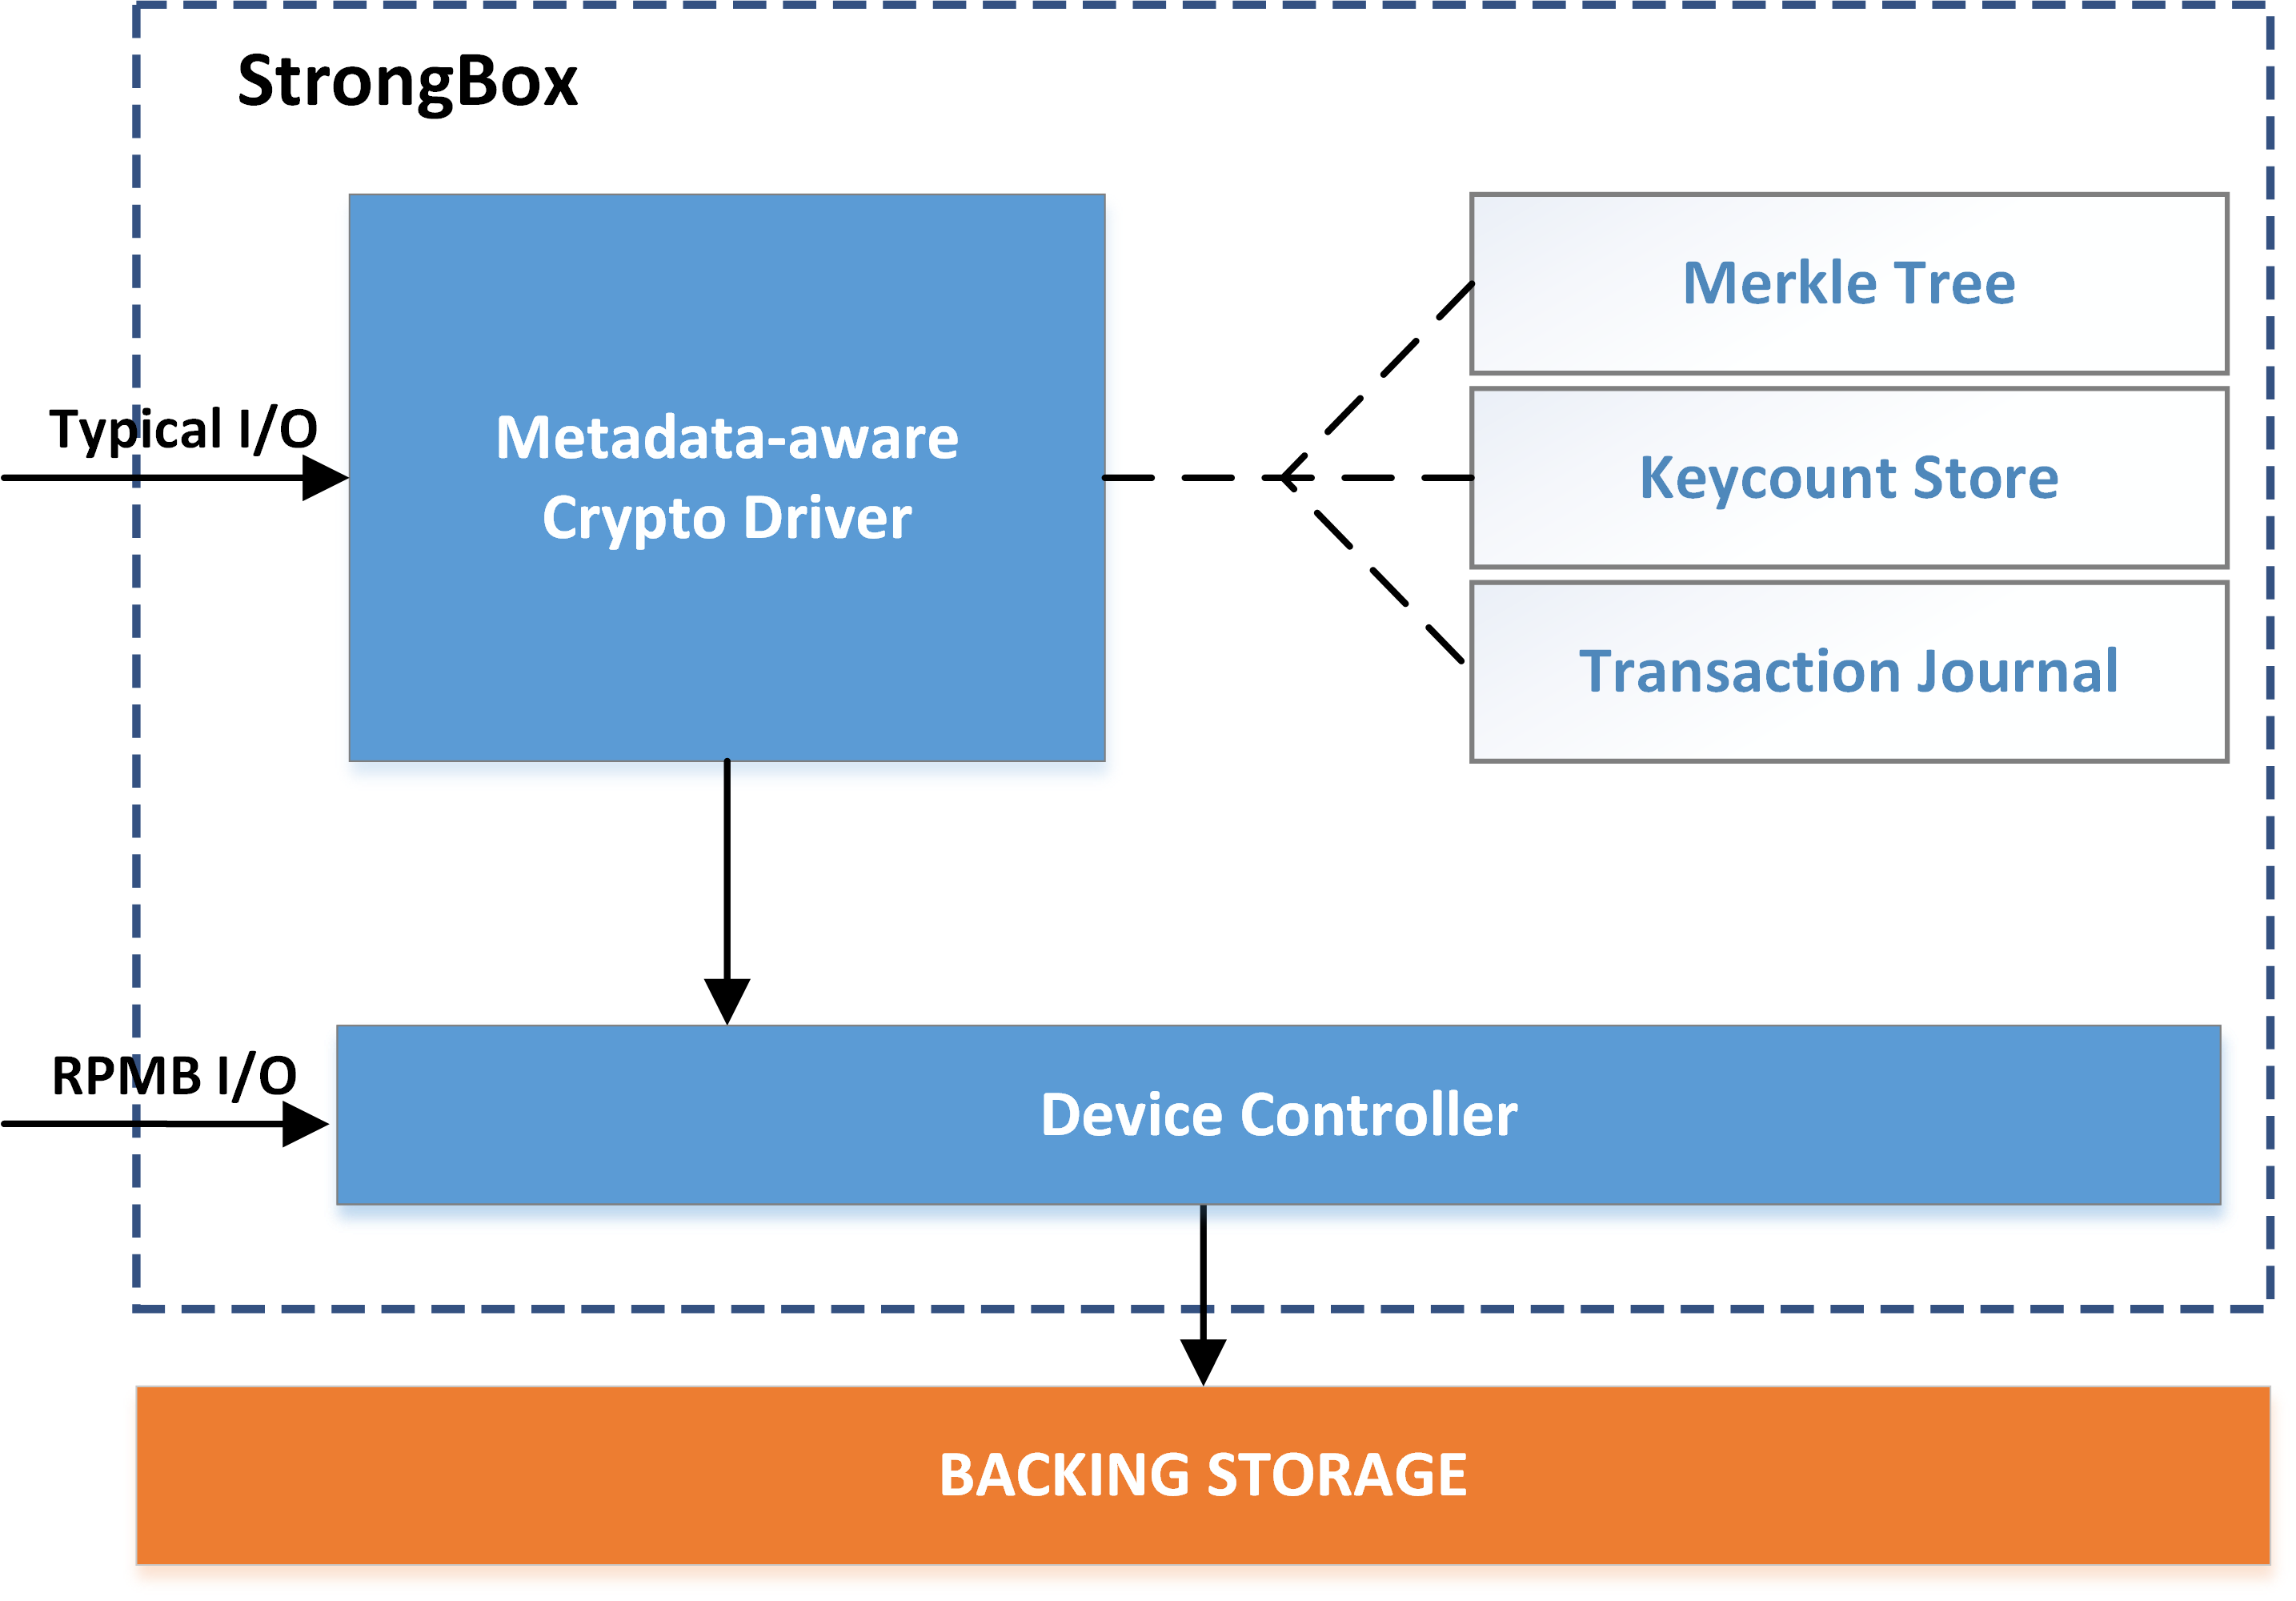
\includegraphics[width=\linewidth]{figs/sc/overview.png}
   \caption{Overview of the SwitchCrypt construction.} \label{fig:overview}
\end{figure}

SwitchCrypt consists of a \emph{Generic Stream Cipher Interface} and
\emph{Cryptographic Driver} and sits between a Log-structured File System (LFS)
on the OS, and the underlying drive (backing storage) and device controller
(e.g. Flash Translation Layer). This is illustrated in \figref{overview}, which
provides an overview of the SwitchCrypt system design.

\begin{figure}[t]
   \centering
   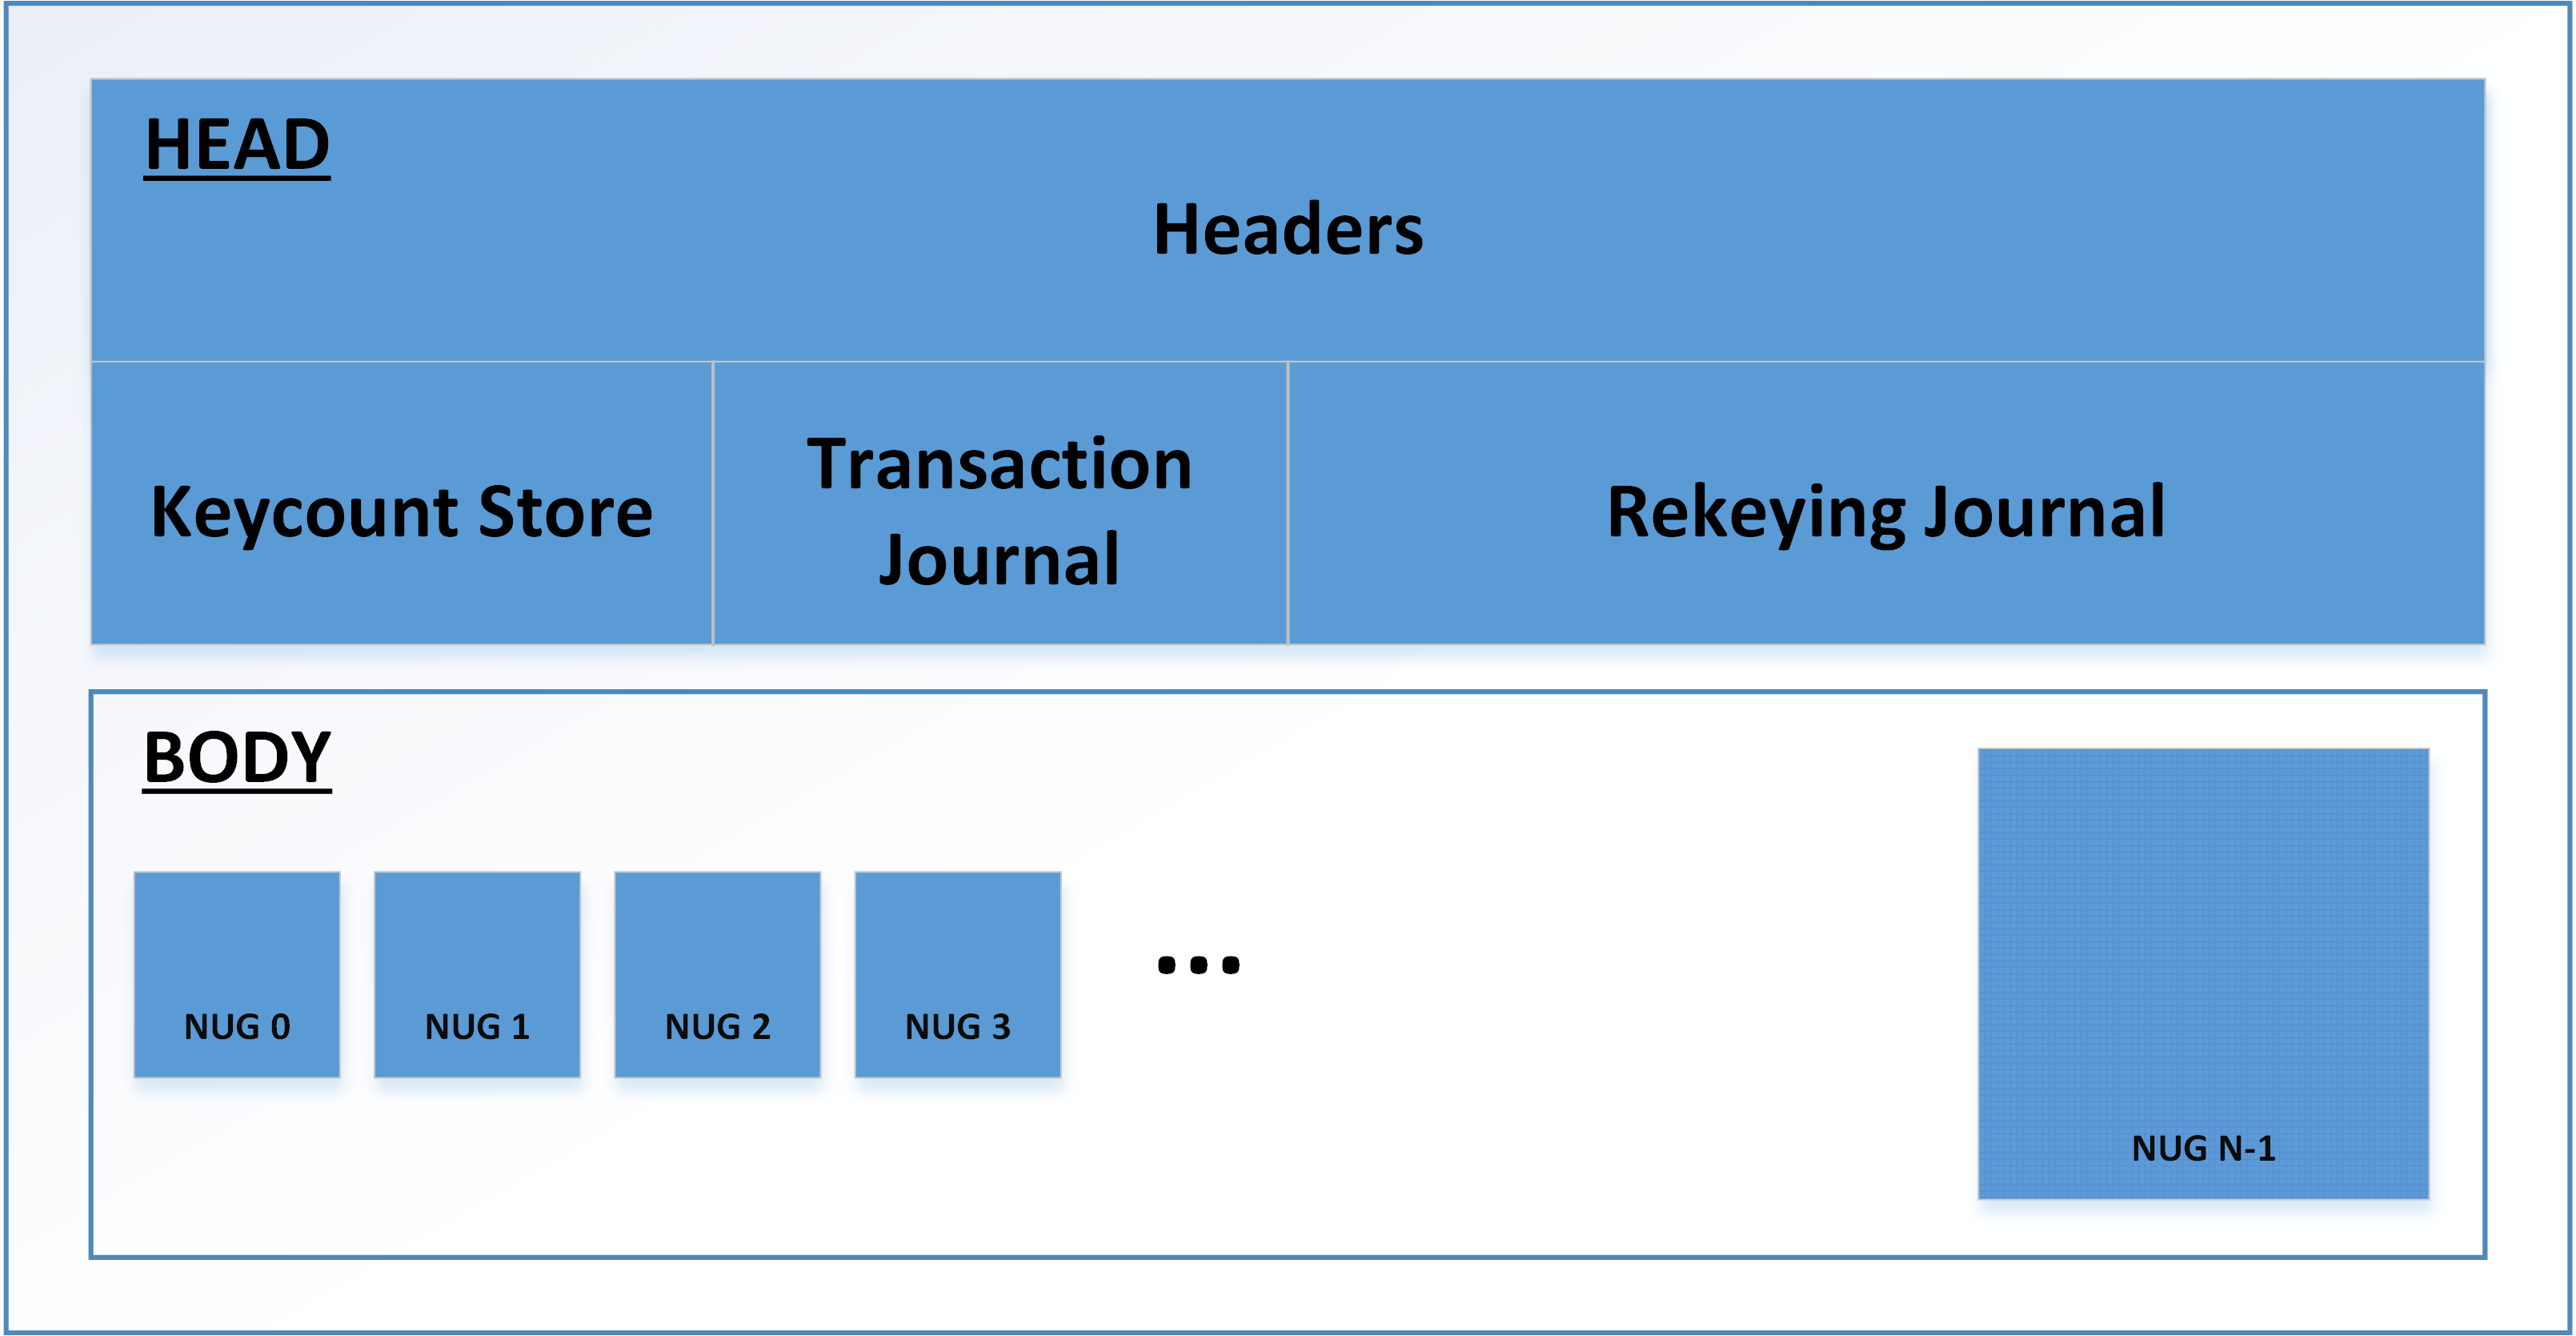
\includegraphics[width=\linewidth]{figs/sc/backstore.png}
   \caption{Layout of SwitchCrypt's drive layout.} \label{fig:backstore}
\end{figure}

The drive itself is divided into a \emph{HEAD} section and \emph{BODY} section
upon initialization, illustrated in \figref{backstore}. The HEAD consists of
metadata headers written during initialization~\cite{StrongBox} along with the
\emph{Keycount Store}, \emph{Transaction Journal}, \emph{Rekeying Journal}, and
\emph{Per-Nugget Metadata}, each drive-backed. These components are used by the
\emph{Cryptographic Driver} together with the \emph{Cipher Switching Strategy}
implementations to enable efficient per-unit cipher switching.

The BODY consists of a series independent same-size logical units called
\emph{nuggets}. A nugget consists of one or more contiguous physical drive
blocks. Each nugget is coupled with metadata in the HEAD indicating which cipher
was used to encrypt the nugget along with any additional ciphertext output; the
latter allows us to treat any non-length-preserving ciphers as if they were
length-preserving. SwitchCrypt uses the Keycount Store and Transaction Journal
components along with our nugget layout to 1) track, detect, and handle
overwrites, 2) limit the maximum length of any plaintext input to ciphers, thus
amortizing the overhead incurred during encryption, and 3) independently and
efficiently switch the cipher used to encrypt individual nuggets.

StrongBox demonstrated how to make nugget-based drive organization secure using
a single stream cipher, ChaCha20, to handle overwrites, prevent rollback
attacks, and limit plaintext length~\cite{StrongBox}. However, StrongBox's was
not designed envisioning the utility in trading off between concerns at the
filesystem or device-mapper level, dynamic cipher switching, or protecting
against attacks on data ``in motion;'' the remainder of this section details the
novel components that enable this functionality. Specifically: how we quantify
the properties traded off between configurations (\cref{subsec:quantify}), the
Generic Stream Cipher Interface and Per-Nugget Metadata components
(\cref{subsec:interface}) which decouple cipher implementations from the
encryption process, and our Cipher Switching Strategy implementations
(\cref{subsec:strategies}) used to efficiently encrypt nuggets with different
ciphers.

\subsection{Quantifying Cipher Security Properties} \label{subsec:quantify}

To reason about when to trade off between the ciphers evaluated in this work, we
must have a way to compare ciphers' utility in the context of SwitchCrypt FDE.
However, different ciphers have a wide range of security properties, performance
profiles, and output characteristics. To address this need, we propose a novel
evaluation framework (see: \tblref{security-quant}). Our framework classifies
stream ciphers according to three quantitative features: relative round count,
ciphertext randomization, and ciphertext expansion. Taken together, these
features reveal a rich tradeoff space of cipher configurations optimizing for
different combinations of concerns.

\begin{table}[ht]
   \centering
   \begin{tabular}{@{}ccccc@{}}
   \toprule
   \textbf{Cipher} & \textbf{Rounds} & \textbf{Randomization} &
   \textbf{Expansion} \\
   \midrule
   ChaCha8         & 0           & 0           & 1           \\
   ChaCha12        & 0.5         & 0           & 1           \\
   ChaCha20        & 1           & 0           & 1           \\
   Salsa8          & 0           & 0           & 1           \\
   Salsa12         & 0.5         & 0           & 1           \\
   Salsa20         & 1           & 0           & 1           \\
   HC128           & 0           & 0           & 1           \\
   HC256           & 1           & 0           & 1           \\
   Freestyle (F)   & 0           & 2           & 0           \\
   Freestyle (B)   & 0.5         & 2.5         & 0           \\
   Freestyle (S)   & 1           & 3           & 0           \\
\end{tabular}
   \caption{Our framework for classifying stream ciphers according to three
   ideal features: relative round count, ciphertext randomization, and
   ciphertext expansion.}
   \label{tbl:security-quant}
 \end{table}

\subsubsection{Relative Rounds (Rounds)}

The ciphers we examine in this work are all constructed around the notion of
\emph{rounds}, where a higher number of rounds (and possibly longer key) is
positively correlated with a higher resistance to brute force given no fatal
related-key or other attacks~\cite{ChaCha-Cryptanalysis}. Hence, this feature
represents how many rounds a cipher executes relative to other implementations
of the same algorithm. For instance: ChaCha8 is a reduced-round version of
ChaCha12, which is a reduced-round version of ChaCha20, all using the ChaCha
algorithm~\cite{ChaCha20,ChaCha-Cryptanalysis}.

We limit our analysis to groups of three implementations, each using a different
number of rounds. In the case of HC-128 and HC-256, we limit our analysis to a
group of two implementations. Scores range from 0 (least number of rounds
considered) to 1 (greatest number of rounds considered).

\subsubsection{Ciphertext Randomization (Randomization)}

A cipher with ciphertext randomization generates different ciphertexts
non-deterministically given the same key, nonce, and plaintext. This makes it
much more difficult to execute chosen-ciphertext attacks (CCA), key
re-installation attacks, XOR-based cryptanalysis and other comparison attacks,
and other confidentiality-violating schemes where the ciphertext is in full
control of the adversary ~\cite{Freestyle}. This property is useful in cases
where we cannot prevent the same key, nonce, and plaintext from being reused,
such as with data ``in motion'' (see the motivational example in
\secref{sc-motivation}). Ciphers without this property---such as ChaCha20 on
which prior work is based---are trivially broken when key-nonce-plaintext
3-tuples are reused. In StrongBox, this is referred to as an ``overwrite
condition'' or simply ``overwrite''~\cite{StrongBox}.

Though there are many ways to achieve ciphertext randomization, the ciphers
included in our analysis implement it using a random number of rounds for each
block of the message where the exact number of rounds are unknown to the
receiver a priori~\cite{Freestyle}. In determining the minimum and maximum
number of rounds used per block in this non-deterministic mode of operation, we
can customize the computational burden an attacker must bear by choosing lower
or higher minimums and maximums. Hence, this is not a binary feature; scores
range from 0 (no ciphertext randomization) to 1 (lowest minimum and maximum
rounds per block) to 3 (highest minimum and maximum rounds per block).

\subsubsection{Ciphertext Expansion (Expansion)}

A cipher that exhibits ciphertext expansion is non-length-preserving: it outputs
more or less ciphertext than was originally input as plaintext. This can cause
major problems in the FDE context. For instance, cryptosystems that rely on
AES-XTS (e.g. Linux's dm-crypt, Microsoft's BitLocker, Apple's FileVault) or
ChaCha (e.g. StrongBox, Google's Adiantum) have storage layouts that hold
length-preserving output as an invariant, making ciphers that do not exhibit
this property incompatible with their implementations; yet, ciphertext expansion
is often (but not always) a necessary side-effect of ciphertext randomization.

The ciphers included in our analysis that exhibit ciphertext expansion have an
overhead of around 1.56\% per plaintext message block~\cite{Freestyle}. Even a
single byte of additional ciphertext vs plaintext would make a cipher
inappropriate for use with prior work. Hence, this is a binary feature in that a
cipher either outputs ciphertext of the same length as its plaintext input or it
does not. A cipher scores either a 0 if it \emph{is not} length-preserving in
this way or a 1 if the ciphertext is always the same length as the plaintext.

\subsection{Generic Stream Cipher Interface} \label{subsec:interface}

One of the goals of SwitchCrypt is that we might use any stream cipher
regardless of its implementation details. Yet this is entirely non-trivial.
There are many cipher implementations that we might use with SwitchCrypt, each
with unique input requirements and output considerations. For instance, Salsa
and Chacha implementations require a certain IV and key size and handle
plaintext input through successive invocations of a single state update
function~\cite{Floodyberry}. Using OpenSSL's AES implementation in CTR mode
requires manually tracking the counter state and individual ciphertext blocks
are retrieved though corresponding function invocations. Freestyle's reference
implementation requires we calculate the extra space necessary per nugget (due
to ciphertext expansion) along with configuration-dependent minimum and maximum
rounds-per-block, hash interval, and pepper bits~\cite{Freestyle}. HC-128 and
other ciphers have similarly disparate requirements.

Unlike prior work, SwitchCrypt must be able to encrypt and decrypt arbitrary
nuggets \emph{with any of these ciphers} at any moment with low overhead and
without tight coupling to any specific implementation detail. Hence, there is a
need for an interface that completely decouples cipher implementations from the
encryption/decryption process. Our novel cipher interface allows any stream
cipher to be integrated into SwitchCrypt without modifications to third-party
code, enabling normally incompatible ciphers to encrypt and decrypt arbitrary
nuggets. The ability for disparate cipher implementations to co-exist forms the
foundation for SwitchCrypt's ability to switch the system between different
cipher configurations in our tradeoff space efficiently and effectively.

To facilitate this, the Generic Stream Cipher Interface presents the
cryptographic driver with a single unified encryption/decryption model.
SwitchCrypt receives I/O requests from the operating system at the block device
level like any other device-mapper. These requests come in the form of either
reads or writes. When a read request is received, the OS hands SwitchCrypt an
offset and a length and expects a response with plaintext of that specific
length starting at that specific offset taken from the beginning of storage
(i.e. the BODY section; see \figref{backstore}). When a write request is
received, the OS hands SwitchCrypt an offset, a length, and a buffer of
plaintext and expects that plaintext to be encrypted and committed to storage
such that the plaintext is later retrievable given that same offset and length
in a future read request. These requests can either be handled together by a
single function or handled individually as distinct read and write operations,
each with different tradeoffs.

\begin{enumerate}
   \item \textbf{\texttt{xor\_interface}}\\\texttt{xor\_interface} executes
   independently of SwitchCrypt internals and treats encryption and decryption
   as the same operation. Implementations receive an integer offset $F$, an
   integer length $L$, a key buffer $K$ corresponding to the current nugget, and
   an empty $L$-length XOR buffer. SwitchCrypt expects the XOR buffer to be
   populated with $L$ bytes of keystream output from some stream cipher seeked
   to offset $F$ with respect to key $K$. The length of the key buffer will
   always be exactly what the cipher implementation expects, alleviating the
   burden of key management; similarly, the XOR buffer will be XOR-ed with the
   appropriate portion of nugget contents automatically, alleviating the burden
   of drive access and other tedious calculations. \\
   \item \textbf{\texttt{read\_interface}} and
   \textbf{\texttt{write\_interface}}\\
   Unlike \texttt{xor\_interface}, encryption and decryption are distinct
   concerns at this abstraction level. \\\texttt{read\_interface} handles
   decryption during reads. \\\texttt{write\_interface} handles encryption
   during writes. Implementations receive full access to SwitchCrypt internals,
   giving wrapper code complete control over the encryption and decryption
   process and allowing implementers to bypass parts of the nugget-based drive
   layout abstraction (i.e. BODY) if necessary. This comes at the cost of 1)
   significantly increased code complexity, as the implementer must perform
   certain I/O manually, distinguish between independent nuggets on the drive,
   determine what to encrypt or decrypt at what offset and when, when to commit
   which metadata and where and 2) potential performance implications, since
   SwitchCrypt must account for not having absolute control over its internal
   data structures during function invocation. For a cipher like Freestyle,
   configurations with lower minimum and maximum rounds per block may see a
   performance improvement here, while configurations with higher minimum and
   maximum rounds per block may see reduced performance.
\end{enumerate}

\subsection{Cipher Switching Strategies} \label{subsec:strategies}

The Generic Stream Cipher Interface allows many differently ciphered nuggets to
co-exist on the same drive. However, at any moment, there is only a single
\emph{active cipher configuration} (henceforth \emph{active configuration}). The
active configuration is used to encrypt nugget contents. When a cipher switch is
triggered, a different configuration becomes the active configuration. At this
point, SwitchCrypt must determine \emph{when} to re-cipher a nugget and
\emph{where} to store the output on the drive. ``Re-ciphering'' here means using
an inactive configuration to decrypt a nugget's contents and using the active
configuration to re-cipher it. Depending on the use case, it may make the most
sense to re-cipher a nugget immediately, or eventually, or to maintain several
areas of differently-ciphered nuggets concurrently.

A naive approach would switch every nugget in BODY to the active configuration
immediately, but the latency and energy cost would be unacceptable. Hence, a
more strategic approach is necessary. We satisfy this need with our \emph{cipher
switching strategies}. These novel strategies allow for nuggets to be
re-ciphered in a variety of cases with minimal impact on performance and battery
life and without compromising security. This is thanks to the nugget-based drive
layout, which limits the churn of cipher switching operations to relatively
small regions of ciphertext on the drive.

Determining \emph{when} to target a nugget for re-ciphering we call
\emph{temporal switching}, for which we propose the \emph{Forward} switching
strategy. Determining \emph{where}---in which storage region and across which
nuggets---to output ciphertext we call \emph{spatial switching}, for which we
propose the \emph{Mirrored} and \emph{Selective} switching strategies. \\

\textbf{Forward Switching Strategy.} When a nugget is encountered during I/O
that was encrypted using something other than the active configuration, the
Forward strategy dictates that this nugget be re-ciphered immediately. If a
particular nugget encrypted with an inactive configuration is never encountered
during I/O, it is never re-ciphered and remains on the drive in its original
state. In this way, the Forward strategy represents a form of temporal cipher
switching.

Rather than re-cipher the entire drive every time the active configuration
changes, this strategy limits the performance impact of cipher switching to
individual nuggets. The expense of re-ciphering is paid only once, after which
the nugget is accessed normally during I/O until the active configuration is
switched again.

There are several forms the Forward strategy might take. The default and
most intuitive is \emph{0-forward}, in which SwitchCrypt immediately transitions
individual nuggets encountered during I/O to the active configuration if they
are not using it. Over time, if various I/O operations end up touching every
nugget in the drive, the encrypted contents of every nugget will become
decryptable with the currently active configuration.

The Forward strategy might also take the form of \emph{N-forward}, where
SwitchCrypt attempts to take advantage of spatial sequential locality to
transition whole sets of nuggets into the active configuration. We can trivially
expand the forward strategy to encompass the entire drive by selecting $N$ equal
to the total number of nuggets managed by SwitchCrypt. This would have the
overhead of re-ciphering large swaths of the drive upon every I/O operation
where a nugget encrypted with the inactive configuration is encountered. Of
course, this has the same dire implications for performance as simply
re-initializing the entire system or encrypted container with the new cipher. \\

\textbf{Selective Switching Strategy.} When SwitchCrypt is initialized with the
Selective strategy, the drive is partitioned into $C$ regions where $C$
represents the total number of available ciphers in the system; each regions'
nuggets are encrypted by each of the $C$ ciphers respectively. For instance,
were SwitchCrypt initialized using two ciphers ($C = 2$), the drive would be
partitioned in half; all nuggets in the first region would be encrypted with the
first cipher while all nuggets in the second would be encrypted with the other.


When using this strategy, the active cipher determines which partition we
``select'' for I/O operations. Hence, unlike the Forward strategy, which
schedules individual nuggets to be re-ciphered at some point in time after the
active configuration is switched, the Selective strategy allows the wider system
to indicate \emph{where} on the drive a read or write operation should occur. In
this way, the Selective strategy represents a form of spatial cipher switching
where different regions of the drive can store differently-ciphered nuggets
independently and concurrently. A user could take advantage of this to, for
instance, set up regions with different security properties and performance
characteristics, managing them as distinct virtual drives or transparently
reading/writing bytes to different security regions on the same drive. \\

\textbf{Mirrored Switching Strategy.} Similar to the Selective strategy, when
SwitchCrypt is initialized with the Mirrored strategy, the drive is partitioned
into $C$ regions where $C$ represents the total number of available ciphers in
the system; each regions' nuggets are encrypted by each of the $C$ ciphers
respectively.

However, unlike the Selective strategy, all write operations that hit one region
are mirrored into the other regions immediately, so all regions of the drive
will always be in a consistent state and always share the same data. The active
configuration determines \emph{where} a read operation should occur. In this
way, the Mirrored strategy represents a form of spatial cipher switching because
we are switching which configuration we are using to read in data. A user could
take advantage of this along with SSD Instant Secure Erase~\cite{ISE1,ISE2,ISE3}
to delete other regions, thus quickly and securely converging the drive to a
single configuration without losing any data or suffering the egregious
performance or battery penalty that comes with re-ciphering every nugget.

\subsubsection{Comparing Cipher Switching Strategies}

\begin{table}[t]
   \centering
   \begin{tabular}{@{}|c|c|c|C{25mm}|@{}}
      \toprule
      \textbf{Strategy} & \textbf{Convergence} & \textbf{Waste} &
      \textbf{Performance} \\
      \midrule
      Forward   & Slower       & None & Faster reads and writes unless switching
      \\\hline
      Mirrored  & Nearly instant & High & Faster reads; slower writes \\
      \hline
      Selective & Slower       & High & Faster reads and writes  \\
      \hline
   \end{tabular}
   \caption{A summary comparison between the three cipher switching strategies.}
   \label{tbl:strategies-advantages}
\end{table}

\tblref{strategies-advantages} summarizes the higher level tradeoffs between the
three cipher switching strategies.

\textbf{Convergence.} Depending on the use case, the ability to quickly converge
the entire drive to a single cipher configuration without losing data is very
useful (see: \secref{sc-usecases}). The near-instantaneous ``just forget the key''
nature of SSD Instant Secure Erase (ISE) implementations on modern
SSDs~\cite{ISE1,ISE2,ISE3} makes this a very fast process for the Mirrored
strategy. The Forward strategy is slow to converge compared to Mirrored since,
in the worse case, every nugget on the drive will require re-ciphering. The
Selective strategy is similarly slow to converge since entire regions of nuggets
must be moved and re-ciphered to prevent data loss; those regions could be
destroyed without moving data around using ISE too, which would be very fast,
but unlike Mirrored some data would be lost forever.

\textbf{Waste.} Unlike the other two strategies, using the Forward strategy does
not reduce the total usable space on the drive by the end-user, ciphertext
expansion notwithstanding. We refer to this as ``waste''. The Forward strategy
is not wasteful in this way because it allows differently-ciphered nuggets to
co-exist contiguously on the drive without special partitions. Since the
Mirrored and Selective strategies require partitioning the drive into some
number of regions---where the writeable size reported back to the OS is some
function of region size---there is a necessary reduction in usable space.

\textbf{Performance.} The Selective and Mirrored strategies can read data from
the drive with low overhead, reaching performance parity with prior work,
because they never have to deal with on-demand re-ciphering. This is because
switching ciphers using these two strategies amounts to offsetting the read
index so that it lands in the proper BODY partition on the drive, which has
little overhead. The Forward strategy also reads with low overhead except in the
case where a nugget was not encrypted with the active configuration. This
triggers re-ciphering on-demand, which can be costly if the workload constantly
touches unique nuggets and is small enough that cost is not amortized.

The Selective strategy also writes with low overhead because, like with reads,
an index offset is the only requirement. The Mirrored strategy, on the other
hand, can be up to two times slower for writes (when $C = 2$) compared to
baseline. Each additional region ($C > 2$) compounds the write penalty depending
on the workload. This is because each write is mirrored across \emph{all}
regions. As with reads, the Forward strategy writes with low overhead except in
the case where a nugget was not encrypted with the active configuration. This
triggers re-ciphering on-demand, which can be costly if the workload touches
unique nuggets and is small enough that cost is not amortized.\\

With these tradeoffs in mind: Mirrored is ideal when the drive must converge
quickly, write performance is not a primary concern, and drive space is
abundant; Selective is ideal when different data should be encrypted differently
and drive space is abundant; and Forward is ideal when some subset of nuggets
should be encrypted differently without wasting drive space. See
\secref{sc-usecases} for specific scenarios that demonstrate these differences in
practice.

\subsubsection{Threat Model for Cipher Switching Strategies}

The primary concern facing any FDE solution is that of confidentiality. An
adversary should not be able to reveal any information about encrypted plaintext
without the proper key. As with prior work, encryption is achieved via a binary
additive approach: cipher output (keystream) is combined with plaintext nugget
contents using XOR, with metadata to track writes and ensure that pad reuse
never occurs during overwrites and that the system can recover from crashes into
a secure state. Another concern is data integrity: an adversary should not be
able to tamper with ciphertext and it go unnoticed. Nugget integrity is tracked
by an in-memory Merkle tree. See the threat model addressed by Dickens et
al.~\cite{StrongBox} for further details.

Switching strategies add an additional security concern not addressed by prior
work: even if we initiate a ``cipher switch,'' there may still be data on the
drive that was encrypted with an inactive configuration. Is this a problem? For
the Forward strategy, this implies data may at any time be encrypted using the
``least desirable cipher''. For the Mirrored and Selective strategies, the drive
is partitioned into regions where nuggets are guaranteed to be encrypted with
each cipher, including the ``least desirable cipher''. However, in terms of
confidentiality, the confidentiality guarantee of SwitchCrypt can be reduced to
the individual confidentiality guarantees of the available ciphers used to
encrypt nuggets.

\subsection{Putting It All Together} \label{subsec:summary}

We revisit the motivating example from \secref{sc-motivation}, where we are
using Freestyle to ensure secure backups. Initially, I/O requests come down from
the LFS and are received by the cryptographic driver, which divides the request
based on which nuggets it touches. For each nugget, the per-nugget metadata is
consulted to determine with which cipher the nugget is encrypted. If it is
encrypted with the active cipher configuration (Freestyle), which must be true
if we have not initiated a cipher switch, the write is handled similarly to
prior work: encrypted data is read in from the drive, the merkle tree and
monotonic counter are consulted to ensure the integrity of encrypted data, the
transaction journal is consulted during write operations so that overwrites are
handled and pad reuse violations are avoided, and then the keycount store is
consulted to derive the nugget's unique encryption key from some master secret.
Finally, using the Generic Stream Cipher Interface, we call out to the
Freestyle, allowing SwitchCrypt to encrypts/decrypts the nugget's contents and
commit any updates back to storage. All the while, the drive's
Freestyle-encrypted contents are being uploaded up to our enterprise backup
service every so often.

When the device enters ``battery saver'' mode, drive backups are paused, the
energy monitoring software downclocks the CPU, and the OS signals to SwitchCrypt
that a more energy-efficient cipher (ChaCha20) should be used until we return to
a non-curtailed energy budget. SwitchCrypt sets ChaCha20 as the active cipher
configuration. Now, when the cryptographic driver divides I/O requests into each
affected nugget, the per-nugget metadata shows SwitchCrypt that each nugget is
encrypted using a cipher that is not the active configuration. This triggers the
re-ciphering code path. Since we are using the Forward switching strategy in
this example, nugget data is immediately decrypted by calling out to the
inactive configuration through the Generic Stream Cipher Interface, after which
the nugget is re-ciphered by calling out to the active configuration. Finally,
the cryptographic driver manages encrypting/decrypting data and updating the
merkle tree and monotonic counter, transaction journal, and keycount store as
the I/O operation and related metadata is committed to the drive afterwards.

Now, thanks to SwitchCrypt, the system can adapt to changing requirements beyond
the capability of prior work. See \secref{sc-usecases} for specifics.

\section{Implementation} \label{sec:hc-implementation}

We implement a proof-of-concept HASCHK frontend as a Google Chrome extension.
To demonstrate the general applicability of our approach, our frontend currently
works with two backends: (1) directly with DNS via Google's JSON API for DNS
over HTTPS (DoH) and (2) indirectly with DHT (Ring OpenDHT) via a local
Representational State Transfer (REST) API we designed to mimic the response
syntax of Google's DoH JSON API. Other candidate backends include storage
clusters, relational and non-relational databases, and any high availability
key-value store.

Our extension operates following the high level overview in \figref{protocol}
with some key implementation-specific functionality that we explore in the
remainder of this subsection. After the user initiates a download either
directly (\eg{ typing a URI manually}) or by following a hyperlink, our
extension, having observed the initial web request, associates that request with
the new download item. The original request may have directly triggered the
download or the download may have been triggered after one or more redirections.
Our extension derives the correct BD in both cases (see below). At this point,
if the backend does not exist or does not conform to the protocol, the protocol
terminates. Otherwise, after the download completes, a URN is calculated and
combined with the BD to make a final query to the backend. In effect, this query
asks: \emph{is this resource compromised?} If the response to the query is
negative (\ie{ a DNS TXT record or DHT data value}), the extension considers the
resource validated. On the other hand, if the response to the query is positive
(\ie{ no record found or bad data value returned}), the extension considers the
resource compromised, deletes the resource file, and warns the user.

In keeping with UX suggestions of prior work, our extension is virtually
transparent to end users in the common case that a download is successfully
verified by a provider's backend or when HASCHK has not been properly
deployed by a provider. However, in the relatively uncommon case that a resource
is deemed compromised, the extension will delete the file and alert the user
with the primary option to ``dismiss'' the alert, mimicking Chrome's own highly
effective dangerous download warning~\cite{ChromeClickThrough}. Specifically:
the user has the option of clicking through the warning via a low-key secondary
interface where they can force the extension to ignore the compromised nature of
the resource \emph{the next time it is downloaded}, forcing the user to trigger
the download again. This inconvenience, favoring users' security over choice, is
in keeping with the recommendations of prior work regarding security warning UX
(see \secref{hc-motivation}).

As no JavaScript OpenDHT client implementation exists, we developed a REST API
to facilitate communication between our extension and the Ring OpenDHT network
via HTTP and JSON. In a production implementation, a JavaScript OpenDHT client
would be baked directly into the extension.

Deploying the DNS backend is as simple as adding certain TXT records to our DNS
zone. This is a straightforward operation. Similarly, deploying the DHT backend
requires adding certain key-value pairs to the OpenDHT network, which is
trivial. Moreover, both DNS and DHT backends are performant and highly
available. The Ring OpenDHT network is also free to use. In the case of DNS, the
vast majority of web-facing providers and IT teams are already using it, already
pay for their own DNS zones, and are already quite familiar with configuring and
managing them. Hence, no exotic secondary backend system is required for
providers with web servers. Additionally, we argue updating the URNs stored by
these backends automatically---by integrating a URN calculation and record
insertion/update step into a modern development toolchain or resource deployment
pipeline---is relatively low-effort and straightforward for providers.

No application or website source code changes, costly user-facing server or web
infrastructure customizations, or modifications to web standards are needed to
enable our extension to protect a provider's resources. Given a production-ready
implementation of our frontend---coupled with the near ubiquitous adoption of
DNS---HASCHK (with a DNS backend) could be deployed immediately by interested
providers.

\subsection{URNs, BDs, and Fallthrough in Google Chrome}

BD derivation in the browser is non-trivial. Users can initiate downloads
through clicking links inside \emph{and outside} the browser (\eg{ in an email
application}), through asynchronous JavaScript, and by entering URIs into the
browser manually. To catch these and other edge cases, we implement our
extension using the WebRequest API~\cite{ExtensionAPI}, which allows us to
monitor all navigation events, collate redirects into an interrogable chain of
requests, and associate new download items with the URI where they were
originally initiated.

To query the backend, we: (1) BASE32 encode the resource's URN. (2) Divide the
112-character result into two 56-character strings \texttt{C1} and \texttt{C2}.
(3) We calculate the BD, which is either the 3LD and 2LD from
\texttt{details.originUrl}. We choose by issuing up to two queries of the form
\texttt{AL.BD}, where the Application Label (AL) is the constant string
\texttt{\_haschk}, looking for a response containing the value \texttt{OK}. We
first query the 3LD as BD and, if we do not receive the proper response there,
query the 2LD as BD. If the proper response is not received from either query,
the extension assumes HASCHK has not been properly deployed and terminates.
(4) Otherwise, concatenating C1, C2, AL, and BD, we issue a query of the form
\texttt{C1.C2.AL.BD}, again looking for a response containing \texttt{OK}
(negative) or that the query was not found (positive).

To handle redirection, we use Chrome's Web Request API to associate redirected
requests with one another. The originating request's \texttt{origin} at the top
of this chain is used to derive the BD using the \texttt{details.originUrl} and
\texttt{details.documentUrl} properties (also avoiding iframe issues). This
prevents an adversary from trivially fooling HASCHK by replacing a legitimate
hyperlink with a malicious one. A naive implementation might use the
\texttt{DownloadItem.referrer} property to derive the BD, since it should be
populated with the originating URL. Unfortunately, this property can be
manipulated with one or more redirections causing the BD to point into the
attacker's DNS zone. If the attacker properly deploys a HASCHK backend, they
could then trivially force false negatives.

Keeping a chain of associated requests also allows us to implement
``fallthrough'' functionality where, if the original request at the head of the
chain has not deployed HASCHK, the extension can walk the chain, checking
each point of redirection for a proper HASCHK deployment. This ensures URL
shorteners and other redirection services do not trigger false positives.

\section{Evaluation} \label{sec:sc-evaluation}

We implement SwitchCrypt and our experiments on a Hardkernel Odroid XU3 ARM
big.LITTLE system with Samsung Exynos 5422 A15/A7 heterogeneous multi-processing
quad core CPUs at maximum clock speed, 2 gigabyte LPDDR3 RAM at 933 MHz, and an
eMMC5.0 HS400 backing store running Ubuntu Trusty 14.04.6 LTS, kernel version
3.10.106. Energy monitoring was provided by the Odroid's integrated INA-231
power sensors polled every $\approx{260}$ milliseconds (not including
noise/overhead).

We evaluate SwitchCrypt using a Linux RAM disk (tmpfs). The maximum theoretical
memory bandwidth for this Odroid model is 14.9GB/s\@. Our observed maximum
memory bandwidth is 4.5GB/s. Using a RAM disk focuses the evaluation on the
performance differences due to different ciphers.

In each experiment below, we evaluate SwitchCrypt on two high level workloads:
sequential and random I/O. In both workloads, a number of bytes are written and
then read (either 4KB, 512KB, 5MB, 40MB) 10 times. Each workload is repeated
three times for a total of 240 tests per cipher (720 runs per cipher
pair/ratios, explained below); 30 results per byte size, 120 results per
workload. Results are accumulated and the median is taken for each byte size.

When evaluating switching strategies, a finer breakdown in workloads is made
using a pre-selected pair of ciphers we call the \emph{primary cipher
configuration} and \emph{secondary cipher configuration}. SwitchCrypt is
initialized at the primary configuration. Once we trigger a cipher switch,
SwitchCrypt moves towards the secondary configuration via switching strategy.

The cipher switch is triggered according to a certain \emph{ratio} of I/O
operations. For example: given 10 40MB read-write operations, we may write and
then read back 40MB 3 times using the primary cipher, initiate a cipher switch,
and then write and then read back (write-read) 40MB 7 times. This would be a 3:7
ratio. It follows that there are three ratios we use to evaluate SwitchCrypt's
performance in this regard: 7:3, 5:5, and 3:7. Respectively, that is 7 file
write-read operation in the primary cipher for every 3 file write-read
operations in the secondary cipher (7:3), 7 file write-read operation in the
primary cipher for every other file write-read operation in the secondary cipher
(5:5), and 3 file write-read operations in the primary cipher for every 7 file
write-read operation in the secondary cipher (3:7).

All experiments are performed with basic Linux I/O commands, bypassing system
caching.

In this section we answer the following questions:

\begin{enumerate}
 \item What shape does the cipher configuration tradeoff space take under our
 workloads? (\cref{subsec:1})
 \item Can SwitchCrypt achieve dynamic security/energy tradeoffs by reaching
 configuration points not accessible with prior work? (\cref{subsec:2})
 \item What is the performance and storage overhead of each cipher switching
 strategy? (\cref{subsec:3})
\end{enumerate}

\subsection{Switching Strategies Under Various Workloads} \label{subsec:1}

\begin{figure}[ht]
  \textbf{Baseline Cipher I/O Performance}\par\medskip
  {\begin{tikzpicture}[baseline]

    \pgfmathsetmacro{\ymax}{1.1} % set the maximum y value
    \pgfmathsetmacro{\ymaxbreak}{1.2} % set the y value at which overflow is drawn

    \begin{groupplot}[
        group style={
            group size=2 by 2,
            xlabels at=edge bottom,
            ylabels at=edge left,
            xticklabels at=edge bottom,
            yticklabels at=edge left,
            vertical sep=25pt,
            horizontal sep=15pt,
        },
        %axis x line*=bottom,
        height=3.5cm,
        width=\linewidth/1.75,
        tick align=outside,
        tick pos=bottom, % make sure ticks only appear at the bottom and left axes
        title style={yshift=-1.5ex},
        tick style={ black },
        y tick label style={ /pgf/number format/fixed, /pgf/number format/precision=0 },
        grid style={ dotted, gray },
        scatter,
        point meta=explicit symbolic,
        scatter/classes={
            c8={mark=square*},
            c20={mark=triangle*},
            ff={mark=diamond*},
            fb={mark=pentagon*},
            fs={mark=otimes}
        },
        %every node near coord/.append style={font=\tiny},
        %
        % magic to make the numbers appear above the overly long bars:
        % visualization depends on={rawy \as \rawy}, % save original y values
        % restrict y to domain*={ % now clip/restrict any y value to ymax
        %     \pgfkeysvalueof{/pgfplots/ymin}:\ymaxbreak
        % },
        % after end axis/.code={ % draw squiggly line indicating break
        %     \draw [semithick, white, decoration={snake,amplitude=0.1mm,segment length=0.75mm,post length=0.375mm}, decorate] (rel axis cs:0,1.01) -- (rel axis cs:1,1.01);
        % },
        % nodes near coords={\color{.!75!black}\pgfmathprintnumber\rawy}, % print the original y values (darkened in case they are too light)...
        % nodes near coords greater equal only=\ymax, % ... but ONLY if they are >= ymax
        % clip=false, % allow clip to protrude beyond ymax
        % Custom stuff to edit per template
        %
        xlabel={\footnotesize Security Score},
        xlabel near ticks,
        %xlabel shift={-1.5mm},
        xmin=0, xmax=4,
        xtick={ 0, 1, 2, 3, 4 },
        xticklabels={ 0,,, 3, \empty },
        %major x tick style=transparent,
        %enlarge x limits=0.2, % add some breathing room along the x axis's sides
        %
        ylabel={\footnotesize Latency (normalized)},
        ylabel near ticks,
        ylabel shift={-1.5mm},
        ymajorgrids=true,
        ymin=0, ymax=\ymax,
        ytick={ 0, 1, \ymax },
        yticklabels={ 0, 1, \empty },
        %yticklabels={ 0, 0.5, 1.5, 2 },
        % extra y ticks={1},
        % extra y tick style={grid=major, grid style={dashed, black}},
        % extra y tick label={\empty},
        %bar width=4.5pt, % change size of bars
        %
        legend cell align=center,
        legend style={ column sep=1ex },
        legend entries={%
            {\scriptsize 4K},
            {\scriptsize 512K},
            {\scriptsize 5M},
            {\scriptsize 40M}
        },
        legend style={
            draw=none,
            legend columns=4,
            at={(1.0,1.35)},
            anchor=south,
        },
    ]
        \nextgroupplot[title={Sequential Reads}]
            \addlegendimage{no markers,red}
            \addlegendimage{no markers,green,dashed}
            \addlegendimage{no markers,blue,dashdotted}
            \addlegendimage{no markers,orange,densely dotted}
            \addplot [thick, red] table [
                meta=cipher,
                x=score,
                y=latency,
                discard if symbol not={iop}{4k-r},
                discard if symbol not={order}{seq},
                col sep=space,
            ] {data/sc/tradeoff-baseline.dat};
            % \label[c8]{fig:tnr:c8}
            % \label[c20]{fig:tnr:c20}
            % \label[ff]{fig:tnr:ff}
            % \label[fb]{fig:tnr:fb}
            % \label[fs]{fig:tnr:fs}
            \addplot [thick, dashed, green] table [
                meta=cipher,
                x=score,
                y=latency,
                discard if symbol not={iop}{512k-r},
                discard if symbol not={order}{seq},
                col sep=space
            ] {data/sc/tradeoff-baseline.dat};
            \addplot [thick, dashdotted, blue] table [
                meta=cipher,
                x=score,
                y=latency,
                discard if symbol not={iop}{5m-r},
                discard if symbol not={order}{seq},
                col sep=space
            ] {data/sc/tradeoff-baseline.dat};
            \addplot [thick, densely dotted, orange] table [
                meta=cipher,
                x=score,
                y=latency,
                discard if symbol not={iop}{40m-r},
                discard if symbol not={order}{seq},
                col sep=space
            ] {data/sc/tradeoff-baseline.dat};
        \nextgroupplot[legend to name={throwaway1}, title={Random Reads}]
            \addplot [thick, red] table [
                meta=cipher,
                x=score,
                y=latency,
                discard if symbol not={iop}{4k-r},
                discard if symbol not={order}{rnd},
                col sep=space,
            ] {data/sc/tradeoff-baseline.dat};
            \addplot [thick, dashed, green] table [
                meta=cipher,
                x=score,
                y=latency,
                discard if symbol not={iop}{512k-r},
                discard if symbol not={order}{rnd},
                col sep=space
            ] {data/sc/tradeoff-baseline.dat};
            \addplot [thick, dashdotted, blue] table [
                meta=cipher,
                x=score,
                y=latency,
                discard if symbol not={iop}{5m-r},
                discard if symbol not={order}{rnd},
                col sep=space
            ] {data/sc/tradeoff-baseline.dat};
            \addplot [thick, densely dotted, orange] table [
                meta=cipher,
                x=score,
                y=latency,
                discard if symbol not={iop}{40m-r},
                discard if symbol not={order}{rnd},
                col sep=space
            ] {data/sc/tradeoff-baseline.dat};
        \nextgroupplot[legend to name={throwaway2}, title={Sequential Writes}]
            \addplot [thick, red] table [
                meta=cipher,
                x=score,
                y=latency,
                discard if symbol not={iop}{4k-w},
                discard if symbol not={order}{seq},
                col sep=space,
            ] {data/sc/tradeoff-baseline.dat};
            \addplot [thick, dashed, green] table [
                meta=cipher,
                x=score,
                y=latency,
                discard if symbol not={iop}{512k-w},
                discard if symbol not={order}{seq},
                col sep=space
            ] {data/sc/tradeoff-baseline.dat};
            \addplot [thick, dashdotted, blue] table [
                meta=cipher,
                x=score,
                y=latency,
                discard if symbol not={iop}{5m-w},
                discard if symbol not={order}{seq},
                col sep=space
            ] {data/sc/tradeoff-baseline.dat};
            \addplot [thick, densely dotted, orange] table [
                meta=cipher,
                x=score,
                y=latency,
                discard if symbol not={iop}{40m-w},
                discard if symbol not={order}{seq},
                col sep=space
            ] {data/sc/tradeoff-baseline.dat};
        \nextgroupplot[legend to name={throwaway3}, title={Random Writes}]
            \addplot [thick, red] table [
                meta=cipher,
                x=score,
                y=latency,
                discard if symbol not={iop}{4k-w},
                discard if symbol not={order}{rnd},
                col sep=space,
            ] {data/sc/tradeoff-baseline.dat};
            \addplot [thick, dashed, green] table [
                meta=cipher,
                x=score,
                y=latency,
                discard if symbol not={iop}{512k-w},
                discard if symbol not={order}{rnd},
                col sep=space
            ] {data/sc/tradeoff-baseline.dat};
            \addplot [thick, dashdotted, blue] table [
                meta=cipher,
                x=score,
                y=latency,
                discard if symbol not={iop}{5m-w},
                discard if symbol not={order}{rnd},
                col sep=space
            ] {data/sc/tradeoff-baseline.dat};
            \addplot [thick, densely dotted, orange] table [
                meta=cipher,
                x=score,
                y=latency,
                discard if symbol not={iop}{40m-w},
                discard if symbol not={order}{rnd},
                col sep=space
            ] {data/sc/tradeoff-baseline.dat};
    \end{groupplot}%
\end{tikzpicture}%
} \caption{Median sequential and random
  write and then read performance baseline.}
 \label{fig:tradeoff-no-ratios}
\end{figure}

\figref{tradeoff-no-ratios} shows the relative round count, ciphertext
randomization, and ciphertext expansion scores versus median normalized latency
tradeoff between different stream cipher configurations for our sequential and
random I/O workloads. Trends for median hold when looking at tail latencies as
well. Each line represents one workload: 4KB, 512KB, 5MB, and 40MB respectively
(see legend). Each symbol represents one of our ciphers: ChaCha8, ChaCha20,
Freestyle Fast, Freestyle Balanced, and Freestyle Strong. Of the ciphers we
tested, those with higher round counts and higher ciphertext randomization
scores resulted in higher latency and increased energy use for I/O operations.
The relationship between these concerns is not simply linear, however, which
exposes a rich tradeoff space.

Besides the 4KB workload, the shape of each workload follows a similar trend,
hence we will focus on 40MB and 4KB workloads going forward. Due to the overhead
of metadata management and the fast completion time of the 4KB workloads
(\ie{little time for amortization of overhead}), ChaCha8 and ChaCha20 take
longer to complete than Freestyle Fast. This advantage is not enough to make
Freestyle Balanced or Secure workloads complete faster than the ChaCha variants,
however.

Though ChaCha8 is faster than ChaCha20, there is some variability in
our timing setup when capturing extremely fast events occurring close together
in time. This is why ChaCha8 sometimes appears with higher latency than ChaCha20
for normalized 4KB workloads. ChaCha8 is not slower than ChaCha20.

\subsection{Reaching Between Static Configuration Points} \label{subsec:2}

\begin{figure}[ht]
  \textbf{Forward Switching I/O Ratio Performance}\par\medskip
  {\begin{tikzpicture}[baseline]

    \pgfmathsetmacro{\ymax}{1.1} % set the maximum y value
    \pgfmathsetmacro{\ymaxbreak}{1.2} % set the y value at which overflow is drawn

    \begin{groupplot}[
        group style={
            group size=2 by 2,
            xlabels at=edge bottom,
            ylabels at=edge left,
            xticklabels at=edge bottom,
            yticklabels at=edge left,
            vertical sep=25pt,
            horizontal sep=15pt,
        },
        %axis x line*=bottom,
        height=3.5cm,
        width=\linewidth/1.75,
        tick align=outside,
        tick pos=bottom, % make sure ticks only appear at the bottom and left axes
        title style={yshift=-1.5ex},
        tick style={ black },
        y tick label style={ /pgf/number format/fixed, /pgf/number format/precision=0 },
        grid style={ dotted, gray },
        scatter,
        point meta=explicit symbolic,
        scatter/classes={
            c8={mark=square*},
            c20={mark=triangle*},
            ff={mark=diamond*},
            fb={mark=pentagon*},
            fs={mark=otimes}
        },
        %every node near coord/.append style={font=\tiny},
        %
        % magic to make the numbers appear above the overly long bars:
        % visualization depends on={rawy \as \rawy}, % save original y values
        % restrict y to domain*={ % now clip/restrict any y value to ymax
        %     \pgfkeysvalueof{/pgfplots/ymin}:\ymaxbreak
        % },
        % after end axis/.code={ % draw squiggly line indicating break
        %     \draw [semithick, white, decoration={snake,amplitude=0.1mm,segment length=0.75mm,post length=0.375mm}, decorate] (rel axis cs:0,1.01) -- (rel axis cs:1,1.01);
        % },
        % nodes near coords={\color{.!75!black}\pgfmathprintnumber\rawy}, % print the original y values (darkened in case they are too light)...
        % nodes near coords greater equal only=\ymax, % ... but ONLY if they are >= ymax
        % clip=false, % allow clip to protrude beyond ymax
        % Custom stuff to edit per template
        %
        xlabel={\footnotesize R+R (norm)},
        xlabel near ticks,
        %xlabel shift={-1.5mm},
        xmin=0, xmax=4,
        xtick={ 0, 0.5, 1, 2, 3, 4 },
        xticklabels={ ,0,,, 1, \empty },
        %major x tick style=transparent,
        %enlarge x limits=0.2, % add some breathing room along the x axis's sides
        %
        ylabel={\footnotesize Latency},
        ylabel near ticks,
        ylabel shift={-1.5mm},
        ymajorgrids=true,
        ymin=0, ymax=\ymax,
        ytick={ 0, 1, \ymax },
        yticklabels={ 0, 1, \empty },
        %yticklabels={ 0, 0.5, 1.5, 2 },
        % extra y ticks={1},
        % extra y tick style={grid=major, grid style={dashed, black}},
        % extra y tick label={\empty},
        %bar width=4.5pt, % change size of bars
        %
        legend cell align=left,
        legend style={ column sep=1ex },
        legend entries={
            {\scriptsize Baseline},
            {\scriptsize Ratios},
            {\scriptsize },
            {\scriptsize },
            {\scriptsize },
            {\scriptsize C8},
            {\scriptsize C20},
            {\scriptsize FF},
            {\scriptsize FB},
            {\scriptsize FS}
        },
        legend style={
            draw=none,
            legend columns=5,
            at={(1.0,1.35)},
            anchor=south,
        },
    ]
        \nextgroupplot[title={Sequential 40M Reads}]
            \addlegendimage{no markers,red}
            \addlegendimage{mark=otimes*,only marks,black}
            \addlegendimage{only marks,mark=square*,white}
            \addlegendimage{only marks,mark=square*,white}
            \addlegendimage{only marks,mark=square*,white}
            \addlegendimage{only marks,mark=square*,red}
            \addlegendimage{only marks,mark=triangle*,red}
            \addlegendimage{only marks,mark=diamond*,red}
            \addlegendimage{only marks,mark=pentagon*,red}
            \addlegendimage{only marks,mark=otimes,red}
            \addplot [thick, red] table [
                meta=cipher,
                x=score,
                y=latency,
                discard if symbol not={iop}{40m-r},
                discard if number not={ratio}{0},
                discard if symbol not={order}{seq},
                col sep=space,
            ] {data/sc/tradeoff-ratios.dat};
            \addplot [only marks] table [
                x=score,
                y=latency,
                discard if symbol not={iop}{40m-r},
                discard if number not={ratio}{1},
                discard if symbol not={order}{seq},
                col sep=space
            ] {data/sc/tradeoff-ratios.dat};
            \addplot [only marks] table [
                x=score,
                y=latency,
                discard if symbol not={iop}{40m-r},
                discard if number not={ratio}{2},
                discard if symbol not={order}{seq},
                col sep=space
            ] {data/sc/tradeoff-ratios.dat};
            \addplot [only marks] table [
                x=score,
                y=latency,
                discard if symbol not={iop}{40m-r},
                discard if number not={ratio}{3},
                discard if symbol not={order}{seq},
                col sep=space
            ] {data/sc/tradeoff-ratios.dat};
        \nextgroupplot[legend to name={throwaway4}, title={Sequential 4K Reads}]
            \addplot [thick, red] table [
                meta=cipher,
                x=score,
                y=latency,
                discard if symbol not={iop}{4k-r},
                discard if number not={ratio}{0},
                discard if symbol not={order}{seq},
                col sep=space,
            ] {data/sc/tradeoff-ratios.dat};
            \addplot [only marks] table [
                x=score,
                y=latency,
                discard if symbol not={iop}{4k-r},
                discard if number not={ratio}{1},
                discard if symbol not={order}{seq},
                col sep=space
            ] {data/sc/tradeoff-ratios.dat};
            \addplot [only marks] table [
                x=score,
                y=latency,
                discard if symbol not={iop}{4k-r},
                discard if number not={ratio}{2},
                discard if symbol not={order}{seq},
                col sep=space
            ] {data/sc/tradeoff-ratios.dat};
            \addplot [only marks] table [
                x=score,
                y=latency,
                discard if symbol not={iop}{4k-r},
                discard if number not={ratio}{3},
                discard if symbol not={order}{seq},
                col sep=space
            ] {data/sc/tradeoff-ratios.dat};
        \nextgroupplot[legend to name={throwaway5}, title={Sequential 40M Writes}]
            \addplot [thick, red] table [
                meta=cipher,
                x=score,
                y=latency,
                discard if symbol not={iop}{40m-w},
                discard if number not={ratio}{0},
                discard if symbol not={order}{seq},
                col sep=space,
            ] {data/sc/tradeoff-ratios.dat};
            \addplot [only marks] table [
                x=score,
                y=latency,
                discard if symbol not={iop}{40m-w},
                discard if number not={ratio}{1},
                discard if symbol not={order}{seq},
                col sep=space
            ] {data/sc/tradeoff-ratios.dat};
            \addplot [only marks] table [
                x=score,
                y=latency,
                discard if symbol not={iop}{40m-w},
                discard if number not={ratio}{2},
                discard if symbol not={order}{seq},
                col sep=space
            ] {data/sc/tradeoff-ratios.dat};
            \addplot [only marks] table [
                x=score,
                y=latency,
                discard if symbol not={iop}{40m-w},
                discard if number not={ratio}{3},
                discard if symbol not={order}{seq},
                col sep=space
            ] {data/sc/tradeoff-ratios.dat};
        \nextgroupplot[legend to name={throwaway6}, title={Sequential 4K Writes}]
            \addplot [thick, red] table [
                meta=cipher,
                x=score,
                y=latency,
                discard if symbol not={iop}{4k-w},
                discard if number not={ratio}{0},
                discard if symbol not={order}{seq},
                col sep=space,
            ] {data/sc/tradeoff-ratios.dat};
            \addplot [only marks] table [
                x=score,
                y=latency,
                discard if symbol not={iop}{4k-w},
                discard if number not={ratio}{1},
                discard if symbol not={order}{seq},
                col sep=space
            ] {data/sc/tradeoff-ratios.dat};
            \addplot [only marks] table [
                x=score,
                y=latency,
                discard if symbol not={iop}{4k-w},
                discard if number not={ratio}{2},
                discard if symbol not={order}{seq},
                col sep=space
            ] {data/sc/tradeoff-ratios.dat};
            \addplot [only marks] table [
                x=score,
                y=latency,
                discard if symbol not={iop}{4k-w},
                discard if number not={ratio}{3},
                discard if symbol not={order}{seq},
                col sep=space
            ] {data/sc/tradeoff-ratios.dat};
    \end{groupplot}
\end{tikzpicture}%
} \caption{Median sequential and random
  write and then read back performance comparison of Forward switching to
  baseline. Each cluster of 3 dots between configurations represents the 7:3,
  5:5, and 3:7 primary-vs-secondary I/O ratios described in the text.}
 \label{fig:tradeoff-with-ratios}
\end{figure}

\figref{tradeoff-with-ratios} shows the relative round count, ciphertext
randomization, and ciphertext expansion scores versus median normalized latency
tradeoff between different stream ciphers for our sequential and random I/O
workloads with cipher switching using the Forward strategy. After a certain
number of write-read I/O operations, a cipher switch is initiated and
SwitchCrypt begins using the secondary cipher to encrypt and decrypt data. For
each pair of ciphers, this is repeated three times: once at every ratio point
\emph{between} our static configuration points (\ie{7:3, 5:5, and 3:7 described
above}).

The point of this experiment is to determine if SwitchCrypt can effectively
transition the drive between ciphers without devastating performance. For the
40MB, 5MB, and 512KB workloads (40MB is shown), we see that SwitchCrypt can
achieve dynamic security/energy tradeoffs reaching points not accessible with
prior work, all with minimal overhead.

Again, due to the overhead of metadata management for non-Freestyle ciphers (see
\secref{sc-implementation}) and the fast completion time of the 4KB workloads
preventing SwitchCrypt from taking advantage of amortization, ChaCha8 and
ChaCha20 take longer to complete than Freestyle Fast for 4KB reads. We also see
very high latency for ratios between Freestyle Fast and Freestyle Strong cipher
configurations. This is because Freestyle is not length-preserving, so extra
write operations must be performed, and the algorithm itself is generally much
slower than the ChaCha variants (see \figref{tradeoff-no-ratios}). Doubly
invoking Freestyle in a ratio configuration means these penalties are paid more
often.

\begin{figure}[ht]
  \textbf{Mirrored/Selective Switching I/O Ratio Performance}\par\medskip
  \centering
  {\begin{tikzpicture}[baseline]

    \pgfmathsetmacro{\ymax}{1.1} % set the maximum y value
    \pgfmathsetmacro{\ymaxbreak}{1.2} % set the y value at which overflow is drawn

    \begin{groupplot}[
        group style={
            group size=2 by 4,
            xlabels at=edge bottom,
            ylabels at=edge left,
            xticklabels at=edge bottom,
            yticklabels at=edge left,
            vertical sep=25pt,
            horizontal sep=15pt,
        },
        %axis x line*=bottom,
        height=3cm,
        width=\textwidth/4,
        tick align=outside,
        tick pos=bottom, % make sure ticks only appear at the bottom and left axes
        title style={yshift=-1.0ex},
        tick style={ black },
        y tick label style={ /pgf/number format/fixed, /pgf/number format/precision=0 },
        grid style={ dotted, gray },
        scatter,
        point meta=explicit symbolic,
        scatter/classes={
            c8={mark=square*},
            c20={mark=triangle*},
            ff={mark=diamond*},
            fb={mark=pentagon*},
            fs={mark=*},
            mirrored={mark=otimes},
            selective={mark=oplus}
        },
        %every node near coord/.append style={font=\tiny},
        %
        % magic to make the numbers appear above the overly long bars:
        % visualization depends on={rawy \as \rawy}, % save original y values
        % restrict y to domain*={ % now clip/restrict any y value to ymax
        %     \pgfkeysvalueof{/pgfplots/ymin}:\ymaxbreak
        % },
        % after end axis/.code={ % draw squiggly line indicating break
        %     \draw [semithick, white, decoration={snake,amplitude=0.1mm,segment length=0.75mm,post length=0.375mm}, decorate] (rel axis cs:0,1.01) -- (rel axis cs:1,1.01);
        % },
        % nodes near coords={\color{.!75!black}\pgfmathprintnumber\rawy}, % print the original y values (darkened in case they are too light)...
        % nodes near coords greater equal only=\ymax, % ... but ONLY if they are >= ymax
        clip=false, % allow clip to protrude beyond ymax
        % Custom stuff to edit per template
        %
        xlabel near ticks,
        %xlabel shift={-5mm},
        xmin=0, xmax=4,
        %%major x tick style=transparent,
        %enlarge x limits=0.2, % add some breathing room along the x axis's sides
        %
        ylabel={\footnotesize Latency (norm)},
        ylabel near ticks,
        %label shift={-1.5mm},
        ymajorgrids=true,
        ymin=0, ymax=\ymax,
        ytick={ 0, 1, \ymax },
        yticklabels={ 0, 1, \empty },
        %yticklabels={ 0, 0.5, 1.5, 2 },
        % extra y ticks={1},
        % extra y tick style={grid=major, grid style={dashed, black}},
        % extra y tick label={\empty},
        %bar width=4.5pt, % change size of bars
        %
        legend cell align=center,
        legend style={ column sep=1ex },
        legend entries={
            {\scriptsize Baseline I/O},
            {\scriptsize SwitchCrypt Ratio Configuration I/O}
        },
        legend style={
            draw=none,
            legend columns=4,
            at={(1.0,1.45)},
            anchor=south,
        },
    ]
        \nextgroupplot[title={40M Mirrored Reads}]
            \addlegendimage{mark=none,red}
            \addlegendimage{mark=otimes,only marks,black}
            \addplot [thick, red] table [
                meta=cipher,
                x=score,
                y=latency,
                discard if symbol not={iop}{40m-r},
                discard if symbol not={ratio}{0},
                discard if symbol not={strategy}{mirrored},
                col sep=space,
            ] {charts/mirrored-selective-baseline.dat};
            \addplot [only marks] table [
                meta=strategy,
                x=score,
                y=latency,
                discard if symbol not={iop}{40m-r},
                discard if symbol not={ratio}{1},
                discard if symbol not={strategy}{mirrored},
                col sep=space
            ] {charts/mirrored-selective-baseline.dat};
            \addplot [only marks] table [
                meta=strategy,
                x=score,
                y=latency,
                discard if symbol not={iop}{40m-r},
                discard if symbol not={ratio}{2},
                discard if symbol not={strategy}{mirrored},
                col sep=space
            ] {charts/mirrored-selective-baseline.dat};
            \addplot [only marks] table [
                meta=strategy,
                x=score,
                y=latency,
                discard if symbol not={iop}{40m-r},
                discard if symbol not={ratio}{3},
                discard if symbol not={strategy}{mirrored},
                col sep=space
            ] {charts/mirrored-selective-baseline.dat};
        \nextgroupplot[legend to name={throwaway19}, title={40M Selective Reads}]
            \addplot [thick, red] table [
                meta=cipher,
                x=score,
                y=latency,
                discard if symbol not={iop}{40m-r},
                discard if symbol not={ratio}{0},
                discard if symbol not={strategy}{selective},
                col sep=space,
            ] {charts/mirrored-selective-baseline.dat};
            \addplot [only marks] table [
                meta=strategy,
                x=score,
                y=latency,
                discard if symbol not={iop}{40m-r},
                discard if symbol not={ratio}{1},
                discard if symbol not={strategy}{selective},
                col sep=space
            ] {charts/mirrored-selective-baseline.dat};
            \addplot [only marks] table [
                meta=strategy,
                x=score,
                y=latency,
                discard if symbol not={iop}{40m-r},
                discard if symbol not={ratio}{2},
                discard if symbol not={strategy}{selective},
                col sep=space
            ] {charts/mirrored-selective-baseline.dat};
            \addplot [only marks] table [
                meta=strategy,
                x=score,
                y=latency,
                discard if symbol not={iop}{40m-r},
                discard if symbol not={ratio}{3},
                discard if symbol not={strategy}{selective},
                col sep=space
            ] {charts/mirrored-selective-baseline.dat};
        \nextgroupplot[legend to name={throwaway20}, title={4K Mirrored Reads}]
            \addplot [thick, red] table [
                meta=cipher,
                x=score,
                y=latency,
                discard if symbol not={iop}{4k-r},
                discard if symbol not={ratio}{0},
                discard if symbol not={strategy}{mirrored},
                col sep=space,
            ] {charts/mirrored-selective-baseline.dat};
            \addplot [only marks] table [
                meta=strategy,
                x=score,
                y=latency,
                discard if symbol not={iop}{4k-r},
                discard if symbol not={ratio}{1},
                discard if symbol not={strategy}{mirrored},
                col sep=space
            ] {charts/mirrored-selective-baseline.dat};
            \addplot [only marks] table [
                meta=strategy,
                x=score,
                y=latency,
                discard if symbol not={iop}{4k-r},
                discard if symbol not={ratio}{2},
                discard if symbol not={strategy}{mirrored},
                col sep=space
            ] {charts/mirrored-selective-baseline.dat};
            \addplot [only marks] table [
                meta=strategy,
                x=score,
                y=latency,
                discard if symbol not={iop}{4k-r},
                discard if symbol not={ratio}{3},
                discard if symbol not={strategy}{mirrored},
                col sep=space
            ] {charts/mirrored-selective-baseline.dat};
        \nextgroupplot[legend to name={throwaway14}, title={4K Selective Reads}]
            \addplot [thick, red] table [
                meta=cipher,
                x=score,
                y=latency,
                discard if symbol not={iop}{4k-r},
                discard if symbol not={ratio}{0},
                discard if symbol not={strategy}{selective},
                col sep=space,
            ] {charts/mirrored-selective-baseline.dat};
            \addplot [only marks] table [
                meta=strategy,
                x=score,
                y=latency,
                discard if symbol not={iop}{4k-r},
                discard if symbol not={ratio}{1},
                discard if symbol not={strategy}{selective},
                col sep=space
            ] {charts/mirrored-selective-baseline.dat};
            \addplot [only marks] table [
                meta=strategy,
                x=score,
                y=latency,
                discard if symbol not={iop}{4k-r},
                discard if symbol not={ratio}{2},
                discard if symbol not={strategy}{selective},
                col sep=space
            ] {charts/mirrored-selective-baseline.dat};
            \addplot [only marks] table [
                meta=strategy,
                x=score,
                y=latency,
                discard if symbol not={iop}{4k-r},
                discard if symbol not={ratio}{3},
                discard if symbol not={strategy}{selective},
                col sep=space
            ] {charts/mirrored-selective-baseline.dat};
        \nextgroupplot[
            legend to name={throwaway15},
            title={40M Mirrored Writes}
        ]
            \addplot [thick, red] table [
                meta=cipher,
                x=score,
                y=latency,
                discard if symbol not={iop}{40m-w},
                discard if symbol not={ratio}{0},
                discard if symbol not={strategy}{mirrored},
                col sep=space,
            ] {charts/mirrored-selective-baseline.dat};
            \addplot [only marks] table [
                meta=strategy,
                x=score,
                y=latency,
                discard if symbol not={iop}{40m-w},
                discard if symbol not={ratio}{1},
                discard if symbol not={strategy}{mirrored},
                col sep=space
            ] {charts/mirrored-selective-baseline.dat};
            \addplot [only marks] table [
                meta=strategy,
                x=score,
                y=latency,
                discard if symbol not={iop}{40m-w},
                discard if symbol not={ratio}{2},
                discard if symbol not={strategy}{mirrored},
                col sep=space
            ] {charts/mirrored-selective-baseline.dat};
            \addplot [only marks] table [
                meta=strategy,
                x=score,
                y=latency,
                discard if symbol not={iop}{40m-w},
                discard if symbol not={ratio}{3},
                discard if symbol not={strategy}{mirrored},
                col sep=space
            ] {charts/mirrored-selective-baseline.dat};
        \nextgroupplot[
            legend to name={throwaway16},
            title={40M Selective Writes}
        ]
            \addplot [thick, red] table [
                meta=cipher,
                x=score,
                y=latency,
                discard if symbol not={iop}{40m-w},
                discard if symbol not={ratio}{0},
                discard if symbol not={strategy}{selective},
                col sep=space,
            ] {charts/mirrored-selective-baseline.dat};
            \addplot [only marks] table [
                meta=strategy,
                x=score,
                y=latency,
                discard if symbol not={iop}{40m-w},
                discard if symbol not={ratio}{1},
                discard if symbol not={strategy}{selective},
                col sep=space
            ] {charts/mirrored-selective-baseline.dat};
            \addplot [only marks] table [
                meta=strategy,
                x=score,
                y=latency,
                discard if symbol not={iop}{40m-w},
                discard if symbol not={ratio}{2},
                discard if symbol not={strategy}{selective},
                col sep=space
            ] {charts/mirrored-selective-baseline.dat};
            \addplot [only marks] table [
                meta=strategy,
                x=score,
                y=latency,
                discard if symbol not={iop}{40m-w},
                discard if symbol not={ratio}{3},
                discard if symbol not={strategy}{selective},
                col sep=space
            ] {charts/mirrored-selective-baseline.dat};
        \nextgroupplot[
            legend to name={throwaway17},
            title={4K Mirrored Writes},
            xlabel={\footnotesize Security Score},
            xtick={ 0, 1, 2, 3, 4 },
            xticklabels={ 0,,, 3, \empty }
        ]
            \addplot [thick, red] table [
                meta=cipher,
                x=score,
                y=latency,
                discard if symbol not={iop}{4k-w},
                discard if symbol not={ratio}{0},
                discard if symbol not={strategy}{mirrored},
                col sep=space,
            ] {charts/mirrored-selective-baseline.dat};
            \addplot [only marks] table [
                meta=strategy,
                x=score,
                y=latency,
                discard if symbol not={iop}{4k-w},
                discard if symbol not={ratio}{1},
                discard if symbol not={strategy}{mirrored},
                col sep=space
            ] {charts/mirrored-selective-baseline.dat};
            \addplot [only marks] table [
                meta=strategy,
                x=score,
                y=latency,
                discard if symbol not={iop}{4k-w},
                discard if symbol not={ratio}{2},
                discard if symbol not={strategy}{mirrored},
                col sep=space
            ] {charts/mirrored-selective-baseline.dat};
            \addplot [only marks] table [
                meta=strategy,
                x=score,
                y=latency,
                discard if symbol not={iop}{4k-w},
                discard if symbol not={ratio}{3},
                discard if symbol not={strategy}{mirrored},
                col sep=space
            ] {charts/mirrored-selective-baseline.dat};
        \nextgroupplot[
            legend to name={throwaway18},
            title={4K Selective Writes},
            xlabel={\footnotesize Security Score},
            xtick={ 0, 1, 2, 3, 4 },
            xticklabels={ 0,,, 3, \empty }
        ]
            \addplot [thick, red] table [
                meta=cipher,
                x=score,
                y=latency,
                discard if symbol not={iop}{4k-w},
                discard if symbol not={ratio}{0},
                discard if symbol not={strategy}{selective},
                col sep=space,
            ] {charts/mirrored-selective-baseline.dat};
            \addplot [only marks] table [
                meta=strategy,
                x=score,
                y=latency,
                discard if symbol not={iop}{4k-w},
                discard if symbol not={ratio}{1},
                discard if symbol not={strategy}{selective},
                col sep=space
            ] {charts/mirrored-selective-baseline.dat};
            \addplot [only marks] table [
                meta=strategy,
                x=score,
                y=latency,
                discard if symbol not={iop}{4k-w},
                discard if symbol not={ratio}{2},
                discard if symbol not={strategy}{selective},
                col sep=space
            ] {charts/mirrored-selective-baseline.dat};
            \addplot [only marks] table [
                meta=strategy,
                x=score,
                y=latency,
                discard if symbol not={iop}{4k-w},
                discard if symbol not={ratio}{3},
                discard if symbol not={strategy}{selective},
                col sep=space
            ] {charts/mirrored-selective-baseline.dat};
    \end{groupplot}
\end{tikzpicture}%
} \caption{Median sequential and
  random write and then read back performance comparison of Mirrored and
  Selective switching strategies to baseline.}
 \label{fig:mirrored-selective-baseline}
\end{figure}

\figref{mirrored-selective-baseline} show the performance of the Mirrored and
Selective strategies with the same configuration of ratios as
\figref{tradeoff-with-ratios}.

For the 40MB, 5MB, and 512KB workloads (40MB is shown), we see that Mirrored and
Selective \emph{read} workloads and the Selective \emph{write} workload achieve
parity with the Forward strategy experiments. This makes sense, as most of the
overhead for Selective and Mirrored reads is determining which part of the drive
to commit data to. The same applies to Selective writes. For the 4KB Mirrored
and Selective \emph{read} workloads and the Selective \emph{write} workload, we
see behavior similar to that in \figref{tradeoff-with-ratios}, as expected.

Mirrored writes across all workloads are very slow. This is to be expected,
since the data is being mirrored across all areas of the drive. In our
experiments, the drive can be considered partitioned in half. This overhead is
most egregious for the 4KB Mirrored write workload. This makes Selective
preferable to Mirrored. However, it is a tradeoff; Selective cannot quickly
converge the drive to a single cipher configuration or survive the loss of an
entire region.

\subsection{Cipher Switching Overhead} \label{subsec:3}

We calculate that Forward switching has average overhead at 0.08x/0.10x for
40MB, 5MB and 512KB read/write workloads compared to baseline I/O, demonstrating
SwitchCrypt's amortization of cipher switching costs. Average overhead
is\\0.38x/0.44x for 4KB read/write workloads when SwitchCrypt is unable to
amortize cost. There is no spatial overhead with the Forward switching strategy.

Similarly, we calculate that Selective switching has average overhead at 0x/0.3x
for 40MB, 5MB and 512KB read/write workloads compared to baseline I/O. Average
overhead is 0.22x/0.71x for 4KB read/write workloads. Spatial overhead in our
experiment was half of all writable space on the drive.

Finally, we calculate that Mirrored switching has average overhead at
0.25x/0.61x for 40MB, 5MB and 512KB read/write workloads compared to baseline
I/O, with high write latency due to mirroring. Average overhead is 0.55x/0.77x
for 4KB read/write workloads. Spatial overhead in our experiment was half of all
writable space on the drive.

These overhead numbers are the penalty paid for the additional flexibility of
being able to reach configurations points that are unachievable without
SwitchCrypt. SwitchCrypt's design keeps these overheads acceptably low in
practice, achieving the desired goal of flexibly navigating latency/security
tradeoffs for FDE.

\subsection{Revisiting Our Threat Model} \label{subsec:4}

The incorporation of cipher switching requires considering each attack in the
context of each strategy and novel attacks on mixed-cipher nugget states.
\tblref{security} lists possible attacks and their results. It can be inferred
from these results and SwitchCrypt's design that SwitchCrypt addresses its
threat model and maintains confidentiality and integrity guarantees. In the case
of the final attack, we stress that even the least scored cipher is still
considered secure (\secref{sc-design}).

\begin{table}[t]
  \caption{Attacks on SwitchCrypt and their results} \label{tbl:security}
  \footnotesize
  \centering
  \begin{tabu} to \linewidth { | X[l] | X[c] | X[c] | }
    \hline
    \textbf{Attack} & \textbf{Result} & \textbf{Explanation} \\
    \hline\hline
    Nugget data in drive is mutated out-of-band online & SwitchCrypt immediately
    fails with exception on successive IO request & Regardless of switching
    strategy, Merkle Tree check fails on read-in\\
    \hline
    Header/cipher metadata in drive is mutated out-of-band online & SwitchCrypt
    immediately fails with exception on successive IO request & Regardless of
    switching strategy, Merkle Tree check fails on read-in\\
    \hline
    drive is rolled back to a previously consistent state while online &
    SwitchCrypt immediately fails with exception on successive IO request &
    Regardless of switching strategy, secure monotonic counter is out of sync
    with the system\\
    \hline
    drive is rolled back to a previously consistent state while offline, secure
    counter wildly out of sync & SwitchCrypt refuses to mount; allows for force
    mount with root access & Regardless of switching strategy, secure monotonic
    counter is out of sync with the system\\
    \hline
    Merkle Tree made inconsistent by mutating drive out-of-band while offline,
    secure counter in sync & SwitchCrypt refuses to mount & Secure monotonic
    counter is in sync with the system, yet illegal data manipulation occurred\\
    \hline
    Nugget accessed out-of-band in mixed-cipher drive & Nugget's cipher may not
    match active configuration & Worst case, the nugget data is available
    encrypted with the lowest scored cipher in the system\\
    \hline\hline
  \end{tabu}
\end{table}


\chapter{Conclusion} \label{chp:conclusion}

The conventional wisdom is that securing data at rest requires one must pay the
high performance overhead of encryption with AES is XTS mode. This work shows
that technological trends overturn this conventional wisdom: log-structured file
systems and hardware support for secure counters make it practical to use a
stream cipher to secure data at rest. We demonstrate this practicality through
our implementation of StrongBox which uses the ChaCha20 stream cipher and the
Poly1305 MAC to provide secure storage and can be used as a drop-in replacement
for dm-crypt.

Our empirical results show that under F2FS---a modern, industrial-strength
Log-structured file system---StrongBox provides upwards of $2\times$ improvement
on read performance and average $1.27\times$ improvement on write performance
compared to dm-crypt. Further, our results show that F2FS plus StrongBox
provides a higher performance replacement for Ext4 backed with dm-crypt. We make
our implementation of StrongBox available open source so that others can extend
it or compare to it.\footnote{\StrongBoxURI} Our hope is that this work
motivates further exploration of fast stream ciphers as replacements for AES-XTS
for securing data at rest.

Further, this work advocates for a more flexible approach to FDE where the
storage system can dynamically adjust the tradeoffs between security and
latency/energy. To support this vision of agile encryption, we proposed an
interface that allows multiple stream ciphers with different input and output
characteristics to be composed in a generic manner. We have identified three
strategies for using this interface to switch ciphers dynamically and with low
overhead. We have also proposed a quantification framework for determining when
to use one cipher over another. Our case studies show how different strategies
can be used to optimize for different goals in practice. We believe that agile
encryption will become increasingly important as successful systems are
increasingly required to balance conflicting operational requirements. We hope
that this work inspires further research in achieving this balance. Our work is
publicly available open-source\footnoteref{note1}.

When it comes to data in motion---specifically, downloading arbitrary resources
over the internet---it is indeed a risky endeavor. Resource integrity and other
Supply Chain Attacks are becoming more frequent and their impact more widely
felt. In this work, we showed that the de facto standard for protecting the
integrity of arbitrary resources on the internet---the use of
\emph{checksums}---is insufficient and often ineffective. We presented HASCHK, a
practical resource verification protocol that automates the tedious parts of
checksum verification while leveraging pre-existing high availability systems to
ensure resources and their checksums are not vulnerable to co-hosting. Further,
we demonstrated the effectiveness and practicality of our approach versus
real-world resource integrity attacks in a production application.

The results of our final evaluation show that our approach is more effective
than checksums and prior work mitigating integrity attacks for arbitrary
resources on the internet. Further, we show HASCHK is capable of guarding
against a variety of attacks, is deployable at scale for providers that already
maintain a DNS presence, and can be deployed without fear of adversely affecting
the user experience of clients that are not HASCHK-aware. Though not a panacea,
we believe our protocol significantly raises the bar for the attacker. We intend
to continue developing our extension and we make it available to a wide audience
(see \cref{app:availability}).

\section{Future Work}

As it stands now, our StrongBox and SwitchCrypt implementations are single
threaded. The cryptographic systems we compared to StrongBox and SwitchCrypt and
all multi-threaded, perhaps making our performance wins more significant. What
performance gains (i.e. more slack) might be available if we parallelize
portions of StrongBox and SwitchCrypt source? Examples include: 1) given that
nuggets are all independent agents, new switching strategies might be developed
that leverage any speedups in parallelizing the encryption and decryption
processes and 2) garbage collection and cipher switching can happen in
background worker threads and could even leverage a scheduler and 3) StrongBox
and SwitchCrypt could be integrated into F2FS directly, sharing its
threading/scheduling model in a production implementation; currently, StrongBox
and SwitchCrypt are implemented on top of the BUSE emulation device.

\renewcommand\thechapter{A}
\chapter{Code Availability} \label{app:availability}

This appendix provides links for the StrongBox, SwitchCrypt, and HASCHK source
code. The two libraries/APIs that StrongBox and SwitchCrypt rely on are
additionally provided. Note that resource locations, URLs, frameworks,
interfaces, etc. will likely change overtime, while this text remains static.

We also make our HASCHK frontend and DHT backend components available open
source for the benefit of the community. We also make publicly available our
evaluation environment: a patched HotCRP instance.

You can find instructions on how to build, test, and modify the StrongBox source
in the provided README documentation linked below. Our hope is that this work
motivates further exploration of resource integrity and other SCA mitigation
strategies and leads to further progress on more exotic FDE schemes.

\begin{table}
    \centering
    \caption{Provides URLs for the products yielded and/or used by this research. The first four URIs refer to repositories on GitHub.}
    \begin{tabular}{|r|c|l|l}
        \cline{1-3}
        \textbf{Project Source} & \textbf{Language} & \textbf{URI} & \\
        \cline{1-3}
        StrongBox Source & C & Xunnamius/strongbox-switchcrypt & \\
        SwitchCrypt Source & C & Xunnamius/strongbox-switchcrypt & \\
        SBD MT Source & C & IAIK/secure-block-device & \\
        BUSE Source & C/Shell & acozzette/BUSE & \\
        HASCHK Source & JavaScript/Shell & https://haschk.dev & \\
        HotCRP Testbed & PHP/C/Shell & https://hotcrp.haschk.dev & \\
        \cline{1-3}
    \end{tabular}
\end{table}


% Format a LaTeX bibliography
\clearpage
\addcontentsline{toc}{chapter}{Bibliography}
\begin{singlespace}
    \printbibliography
\end{singlespace}

% Figures and tables, if you decide to leave them to the end
%\input{figure}
%\input{table}

\end{document}
